%!TEX root = ../main.tex

\chapter{Valutazione delle prestazioni di un classificatore}
\label{cap:prestazioni}

Dato un classificatore supervisionato, addestrato su un \emph{training set}, è fondamentale saper valutare l'accuratezza che può essere ottenuta quando tale classificatore è applicato a campioni incogniti.\\
A tale scopo, è essenziale valutare la probabilità di errore $P_e$ del classificatore per decidere, ad esempio, se le \emph{feature} utilizzate siano sufficienti a discriminare bene le classi o se sia necessario estrarne altre (come parametri di tessitura nel caso in cui i canali spettrali non siano abbastanza discriminanti).
\clearpage

\section{Stima della probabilità di errore}
In presenza di $C$ classi $\omega_1,\omega_2, \ldots, \omega_C$, detta $P_i$ la probabilità \emph{a priori}, la probabilità di errore $P_e$ si può esprimere nel modo seguente:
\begin{equation}
\label{eq:P_e}
P_e = P\lbrace\widehat{Y}\neq Y\rbrace= {\sum_{i=1}^C P\lbrace\widehat{Y}\neq \omega_i\vert Y = \omega_i\rbrace}P\lbrace Y =\omega_i\rbrace
\end{equation}
dove $Y$ è l'etichetta di classe corrispondente alla realtà a terra e $\hat{Y}$ è l'etichetta stimata dal classificatore.
Dal momento che tale espressione è calcolabile solo in pochissimi casi semplici, per valutarla si adotta generalmente un approccio empirico, che stima la $P_e$ come la percentuale dei pixel di test classificati erroneamente.\\
Solitamente la $P_e$ viene valutata su un insieme di campioni pre-etichettati(\emph{test set}) diverso rispetto a quello utilizzato per addestrare il classificatore(\emph{training set}). Questa tecnica, detta \emph{hold-out}, permette una misura delle prestazioni priva di \emph{bias} in quanto eseguita su istanze non utilizzate in fase di apprendimento.\\
Per poter individuare e possibilmente evitare il fenomeno dell'\emph{overfitting},\footnote{Si parla di \emph{overfitting} quando la funzione discriminante è strettamente dipendente dai campioni di \emph{training} specifici utilizzati per calcolarla ed è quindi particolarmente inefficace quando applicata a campioni incogniti} una condizione fondamentale per stimare $P_e$ come frequenza relativa degli errori sul \emph{test set} è che i campioni pre-etichettati siano indipendenti e identicamente distribuiti (i.i.d). Per questa ragione, è buona norma prelevare i campioni di \emph{training} e di \emph{test} in regioni dell'immagine spazialmente disgiunte tra loro.\\
E' altrettanto importante effettuare un'analisi qualitativa dell'intera mappa, mediante foto-interpretazione, come complemento alla valutazione quantitativa delle prestazioni di classificazione sui campioni di test.

\section{Matrice di confusione e parametri di accuratezza}
La $P_e$ fornisce una valutazione complessiva delle prestazioni del classificatore, senza però differenziare gli errori commessi in corrispondenza di classi diverse. Per una valutazione più dettagliata la matrice di confusione (\emph{confusion matrix}) è la tipologia di osservazione statistica maggiormente utilizzata: il risultato della classificazione sulle aree campione viene confrontato con la verità al suolo. Questa è una matrice $C \times C$, il cui elemento $e_{ij}$ è il numero di pixel di test della classe $\omega_i$ che il classificatore ha assegnato alla classe $\omega_j$. Sulla diagonale $i=j$ della matrice di confusione si leggono dunque i numeri di pixel di test classificati in modo corretto. Questo tipo di analisi statistica consente non solo di quantificare il successo ottenuto dalla procedura, ma anche di focalizzare i punti critici del processo di classificazione, ovvero le classi meno distinguibili tra loro. \\
L'accuratezza della classificazione può essere valutata con diversi parametri numerici, tra cui i più utilizzati sono i seguenti:
\begin{itemize}
\item La \emph{Producer Accuracy} (PA) di una classe $\omega_i$ è la
parte di pixel ben classificati rispetto al numero totale di
pixel di test di $\omega_i$, in particolare essa si può esprimere
come:
\begin{equation}
\label{eq:PA}
PA_i=\dfrac{e_{ii}}{\sum_{j=1}^Ce_{ij}}
\end{equation}
Analogamente, si può definire \emph{Omission Error} (OE) di $\omega_i$ la frazione complementare di pixel classificati erroneamente.
\item L' \emph{average accuracy} (AA) delle C classi è la media delle C \emph{producer accuracy} ed è data da:
\begin{equation}
\label{eq:AA}
AA=\dfrac{1}{C}\sum_{i=1}^C{PA_i}
\end{equation}
\item L'\emph{overall accuracy }(OA) è la percentuale di pixel classificati correttamente sull'intero test set ed è data da:
\begin{equation}
\label{eq:OA}
OA= \dfrac{1}{t}\sum_{i=1}^C e_{ij}
\end{equation}
dove $t$ è il numero di pixel di test.
\item Il parametro "$\kappa$", rappresenta una modifica dell' OA finalizzata a tenere conto in modo più completo della distribuzione degli errori tra le diverse classi, ed è dato da:
\begin{equation}
\label{eq:K}
\kappa=\dfrac{OA-\frac{1}{t^2}\sum_{i=1}^C\sum_{j=1}^C\sum_{k=1}^C e_{ij}e_{ki}}{1-\frac{1}{t^2}\sum_{i=1}^C\sum_{j=1}^C\sum_{k=1}^C e_{ij} e_{ki}}
\end{equation}
dove $t$ rappresenta ancora il numero di pixel di test utilizzati.
\end{itemize}


\chapter{Risultati sperimentali} % Main chapter title

\label{cap:risultati} % Change X to a consecutive number; for referencing this chapter elsewhere, use \ref{ChapterX}

%\lhead{Capitolo \ref{chapter_Risultati_sperimentali}. \emph{Risultati sperimentali}} % Change X to a consecutive number; this is for the header on each page - perhaps a shortened title

In questo capitolo verranno presentati tre casi di studio e verrà fatta un'analisi delle prestazioni al variare dei parametri dell’algoritmo  HOG, evidenziando i valori ottimali individuti. 
Successivamente verranno presentati i risultati ottenuti valutando anche gli aspetti per cui questo algoritmo ha dato risultati parzialmente soddisfacenti.

\clearpage

\section{Descrizione dei \emph{dataset}}
In questa tesi sono stati analizzati tre casi rilevanti, tutti relativi alla classificazione dell'area urbana di Amiens (Francia).  Si tratta di un problema di classificazione interessante e particolarmente complesso, in quanto le regioni coinvolte sono caratterizzate sia da aree omogenee (come corsi d'acqua) sia da strutture geometriche ben definite (come edifici e strade) e zone di suolo con\emph{ pattern} regolari (come campi coltivabili e non).\\
L'analisi condotta ha coinvolto l'uso di immagini ad elevata risoluzione spaziale, acquisite nell'ambito di un progetto europeo dedicato allo sviluppo di tecnologie ICT innovative per l'identificazione di aree urbane attualmente non usate e potenzialmente riqualificabili.\\

Il \emph{dataset} per ogni esperimento è costituito da un'immagine telerilevata, dalla mappa di \emph{training} e dalla mappa di \emph{testing} corrispondenti.
Le immagini telerilevate sono state acquisite dal sensore passivo \textsc{SPOT5 HRG} a tre canali, corrispondenti alle lunghezze d'onda del verde (G, $495 - 570\text{ } nm$), del rosso (R, $620 -  750\text{ } nm$) e del vicino infrarosso (NIR, \emph{Near InfraRed} $0.75 - 1.4\text{ } \mu m$).
Sebbene i canali spettrali di SPOT5 HRG avrebbero risoluzione spaziale nativa di 10 m, il sensore stesso acquisisce anche un canale pancromatico, associato all'intero intervallo di lunghezza d'onda (dal visibile al vicino infrarosso) e caratterizzato da risoluzione spaziale di 5 m. In fase di pre-elaborazione, tecniche di \emph{pansharpening}\footnote{Pansharpening è un processo di fusione di immagini pancromatiche ad alta risoluzione con immagini multispettrale a risoluzione inferiore per creare una singola immagine multispettrale ad alta risoluzione.} sono state applicate al fine di fondere le informazione fornite dai dati multispettrali e pancromatici e generare un'immagine G-R-NIR a risoluzione spaziale di 5 m. Inoltre, SPOT5 HRG permette anche acquisizioni di coppie stereo di immagini. L'applicazione di tecniche di super-risoluzione ad una di tali coppie permette di generare un'ulteriore immagine volta a stimare la distribuzione spaziale della radianza ricevuta ad una risoluzione di 2.5 m. Sono stati usati a fini di sperimentazione dati ottenuti da entrambe le tipologie di pre-elaborazione e quindi caratterizzati da pixel di dimensione pari a 2.5 e 5 m.
 

\subsection{Amiens 2006 - 5m - 10 classi}
L'immagine \emph{Amiens6--5m} è stata acquisita nel 2006 e ha pixel di dimensione spaziale pari a $5 \text{m}$, coprendo approssimativamente un'area di $10\text{ }km\times11\text{ }km$ ($2000\times2200$ pixel).\\
L'insieme delle classi $\Omega=\left\lbrace\omega_1,\omega_2,\ldots,\omega_{10}\right\rbrace$ che costituisce questo primo esperimento è il seguente:
\begin{enumerate}
\item Area urbana ad alta densità
\item Area urbana a bassa densità
\item Strade
\item Area verde urbana 
\item Suolo nudo
\item Terreno coltivabile
\item Aree vegetate
\item Alberi
\item Corsi d'acqua
\item Specchi d'acqua
\end{enumerate}
Nella Figura \ref{fig: Amiens65m} vengono presentate le immagini caratterizzanti il primo \emph{dataset}. 
\begin{lstlisting}[float=b,title={Distribuzione dei pixel di training (TR) e test (TE) classe per classe.},
                   label=lst:esempio, frame=lines]
TR:				TE:
Class 1 : 72483 		Class 1 : 70299
Class 2 : 149917 	Class 2 : 68435
Class 3 : 17945 		Class 3 : 10019
Class 4 : 25121 		Class 4 : 16012
Class 5 : 233481 	Class 5 : 115570
Class 6 : 113030 	Class 6 : 48615
Class 7 : 62854 		Class 7 : 54582
Class 8 : 90718 		Class 8 : 50701
Class 9 : 7903 		Class 9 : 3012
Class 10: 34833 		Class 10: 27924
Total   : 808285		Total   : 465169
\end{lstlisting}
\clearpage
\begin{figure}[!ht]
   \center
   \subfigure[Immagine telerilevata]{
      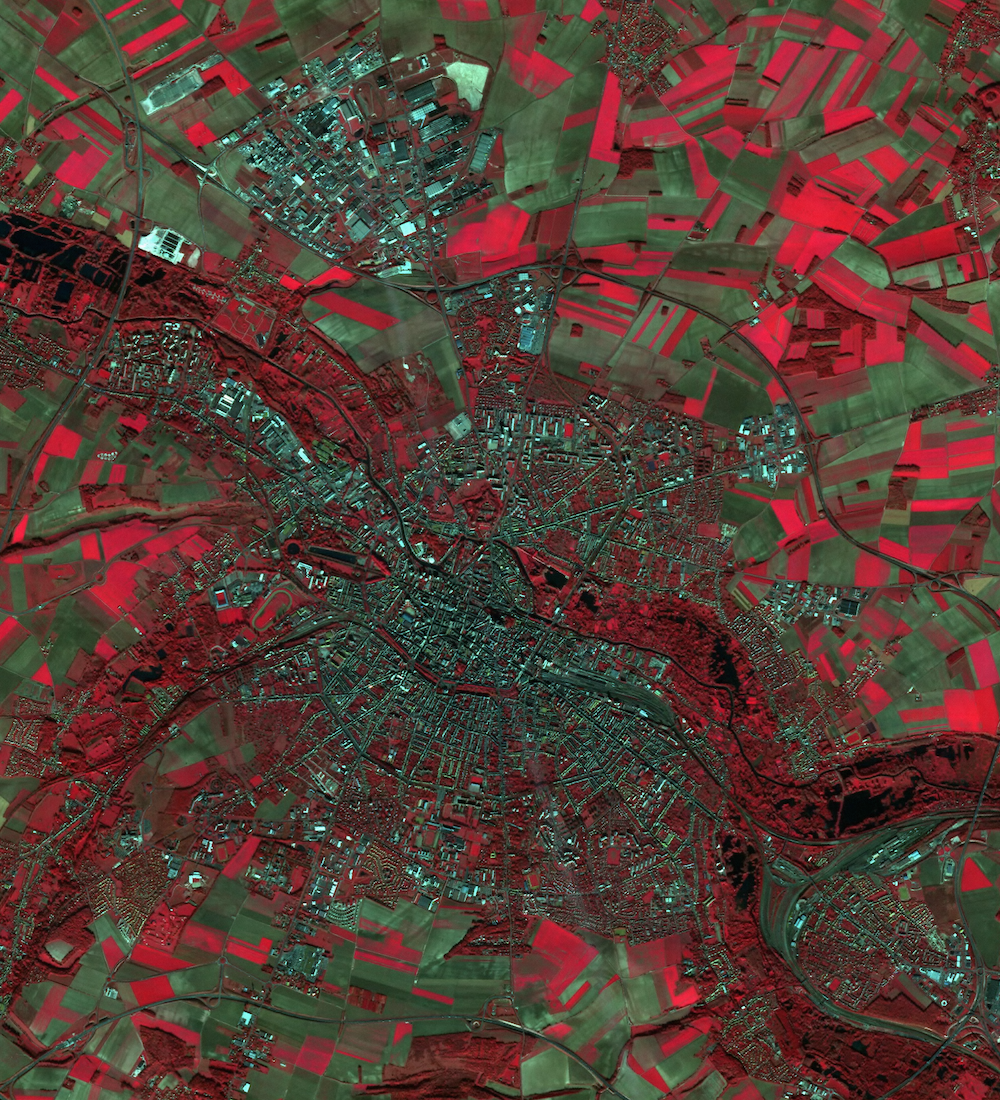
\includegraphics[width=0.7\textwidth]{Amiens_2006_SPOT_5m}}\\%pdf0.45
         \subfigure[Mappa di \emph{training}]{
      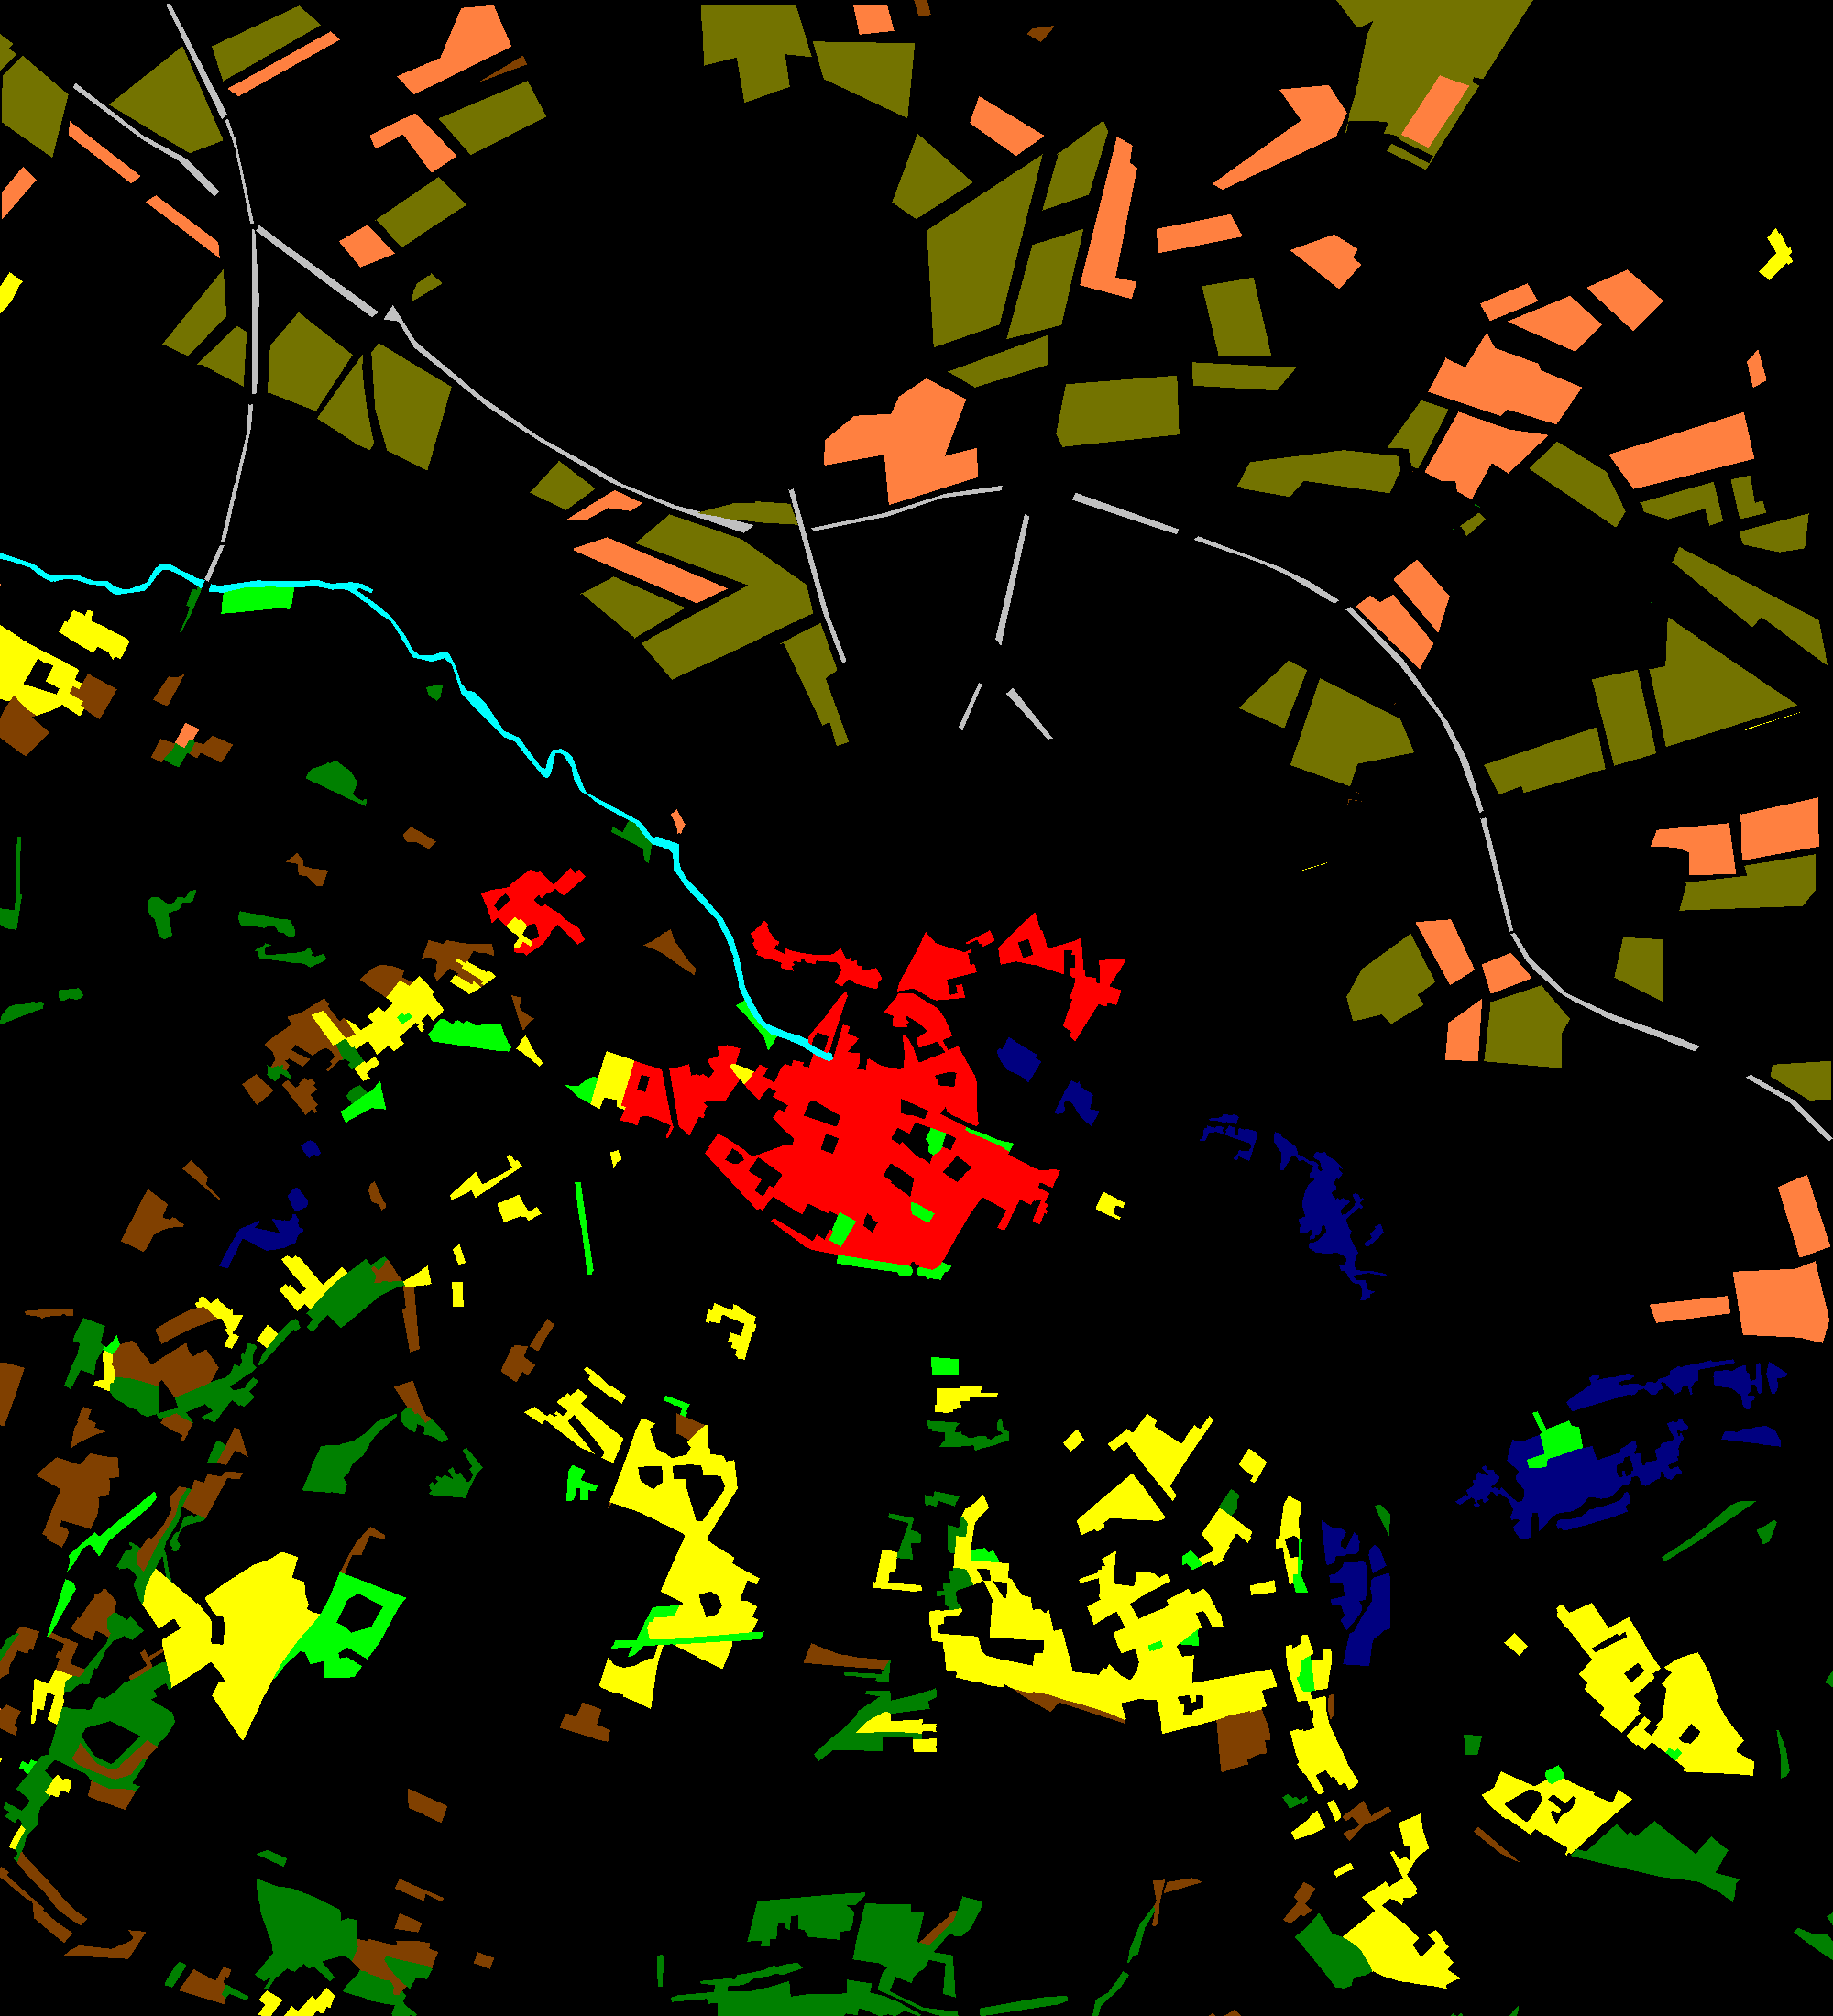
\includegraphics[width=0.4\textwidth]{GT_Amiens2006_5m_10classes_TR}}
     \hspace{4mm}
    \subfigure[Legenda classi della mappa di \emph{training}]{
      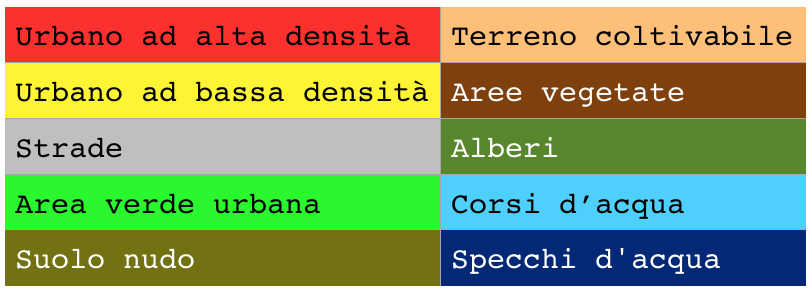
\includegraphics[scale=0.5]{Leggenda_2006_10classi}}
    \caption{\emph{Dataset} con composizione RBG in falso colore ($2000\times2200$ pixel) acquisita su Amiens (Francia) dal sensore \textsc{SPOT5 HRG}}
    \label{fig: Amiens65m}
  \end{figure}
  
\clearpage
\subsection{Amiens 2006 - 2.5m - 7 classi}
L'immagine \emph{Amiens6--2.5m} è stata acquisita sempre nel 2006, ma ha pixel di dimensione spaziale pari a $2.5\text{ }m$  e copre sempre approssimativamente un'area di $10\text{ }km\times11\text{ }km$ ($4001\times4400$ pixel).\\
L'insieme delle classi $\Omega=\left\lbrace\omega_1,\omega_2,\ldots,\omega_{7}\right\rbrace$ che costituisce il secondo \emph{dataset} è il seguente:
\begin{enumerate}
\item Edifici
\item Strade e marciapiedi
\item Aree vegetate
\item Suolo nudo
\item Terreno coltivabile
\item Alberi
\item Acqua
\end{enumerate}
Nella Figura \ref{fig: Amiens62_5m} vengono presentate le immagini caratterizzanti il secondo \emph{dataset}. Nella Figura \ref{fig:3classi} sono riportate, per una migliore comprensione, la distribuzione dei pixel di\emph{ training} di tre classi diverse (nero = strade, blu = acqua, verde = aree vegetate), rispetto a due distinte coppie di \emph{feature} spettrali. Tali grafici evidenziano come alcune classi siano spettralmente molto sovrapposte e confermano l'opportunità dell'estrazione di \emph{feature} aggiuntive associate alla distribuzione spaziale delle intensità dei pixel invece che all'informazione spettrale da essi apportata. Inoltre è importante notare come l'immagine a 2.5 m sia visibilmente più sfocata di quella a 5 m. Ciò è legato all'efficacia solo parziale del metodo di super-risoluzione che, in fase di pre-elaborazione, fu applicato. Pertanto, la risoluzione spaziale di tale immagine, ossia la dimensione del più piccolo dettaglio distinguibile, si ritiene peggiore di 2.5 m. Ciò rende il processo di classificazione ulteriormente complesso.

 \begin{figure}[!ht]
\center  
\subfigure{
      \includegraphics[width=0.35\textwidth]{AssiRG_3classi}}
      \hspace{3mm}
\subfigure{ 
		 \includegraphics[width=0.35\textwidth]{AssiGB_3classi}}
		
    \caption{Analisi della distribuzione dei campioni di training di tre classi nelle proiezioni su due diversi sottospazi delle feature}
    \label{fig:3classi}
  \end{figure}


\clearpage

\begin{figure}[!ht]
   \center
   \subfigure[Immagine telerilevata]{
      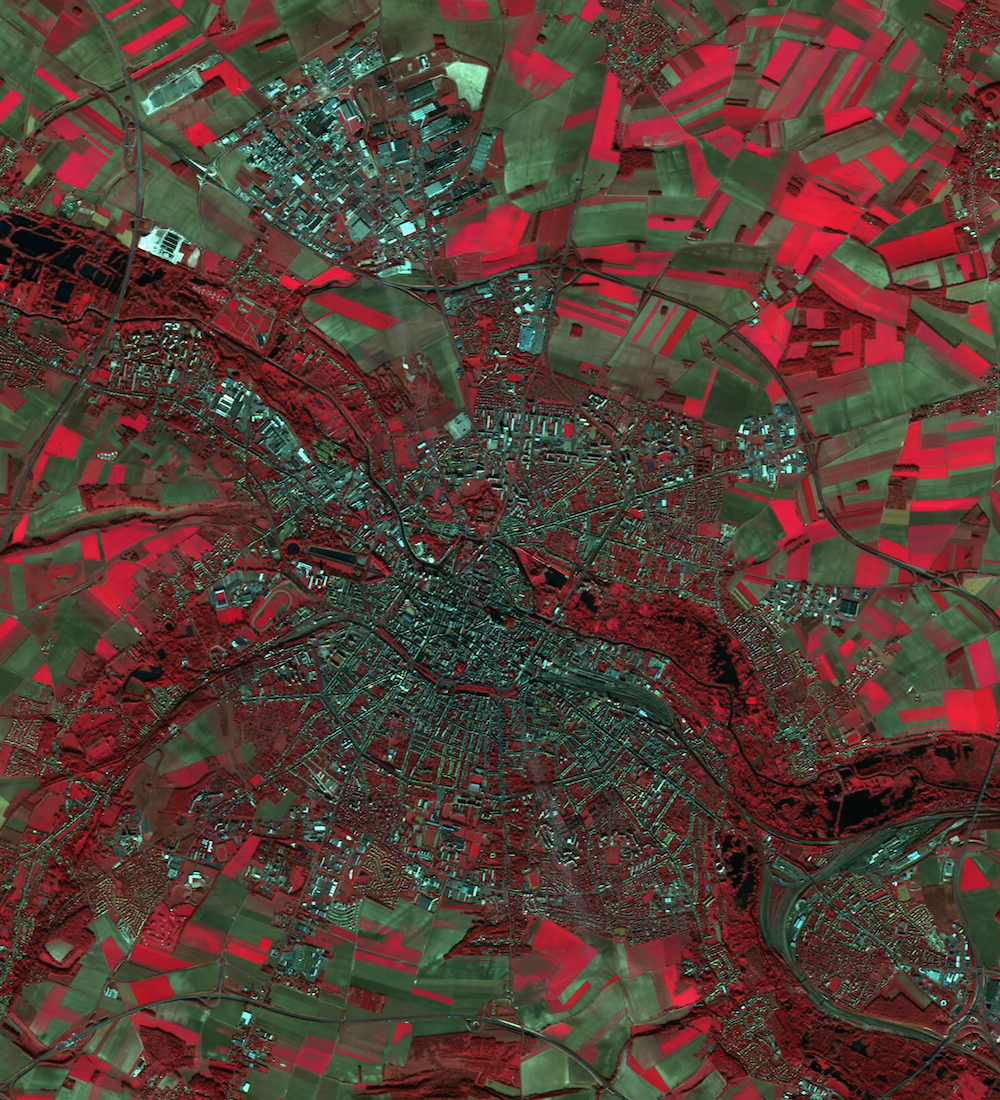
\includegraphics[width=0.7\textwidth]{Amiens_2006_SPOT_2_5m}}\\%pdf0.45
         \subfigure[Mappa di \emph{training}]{
      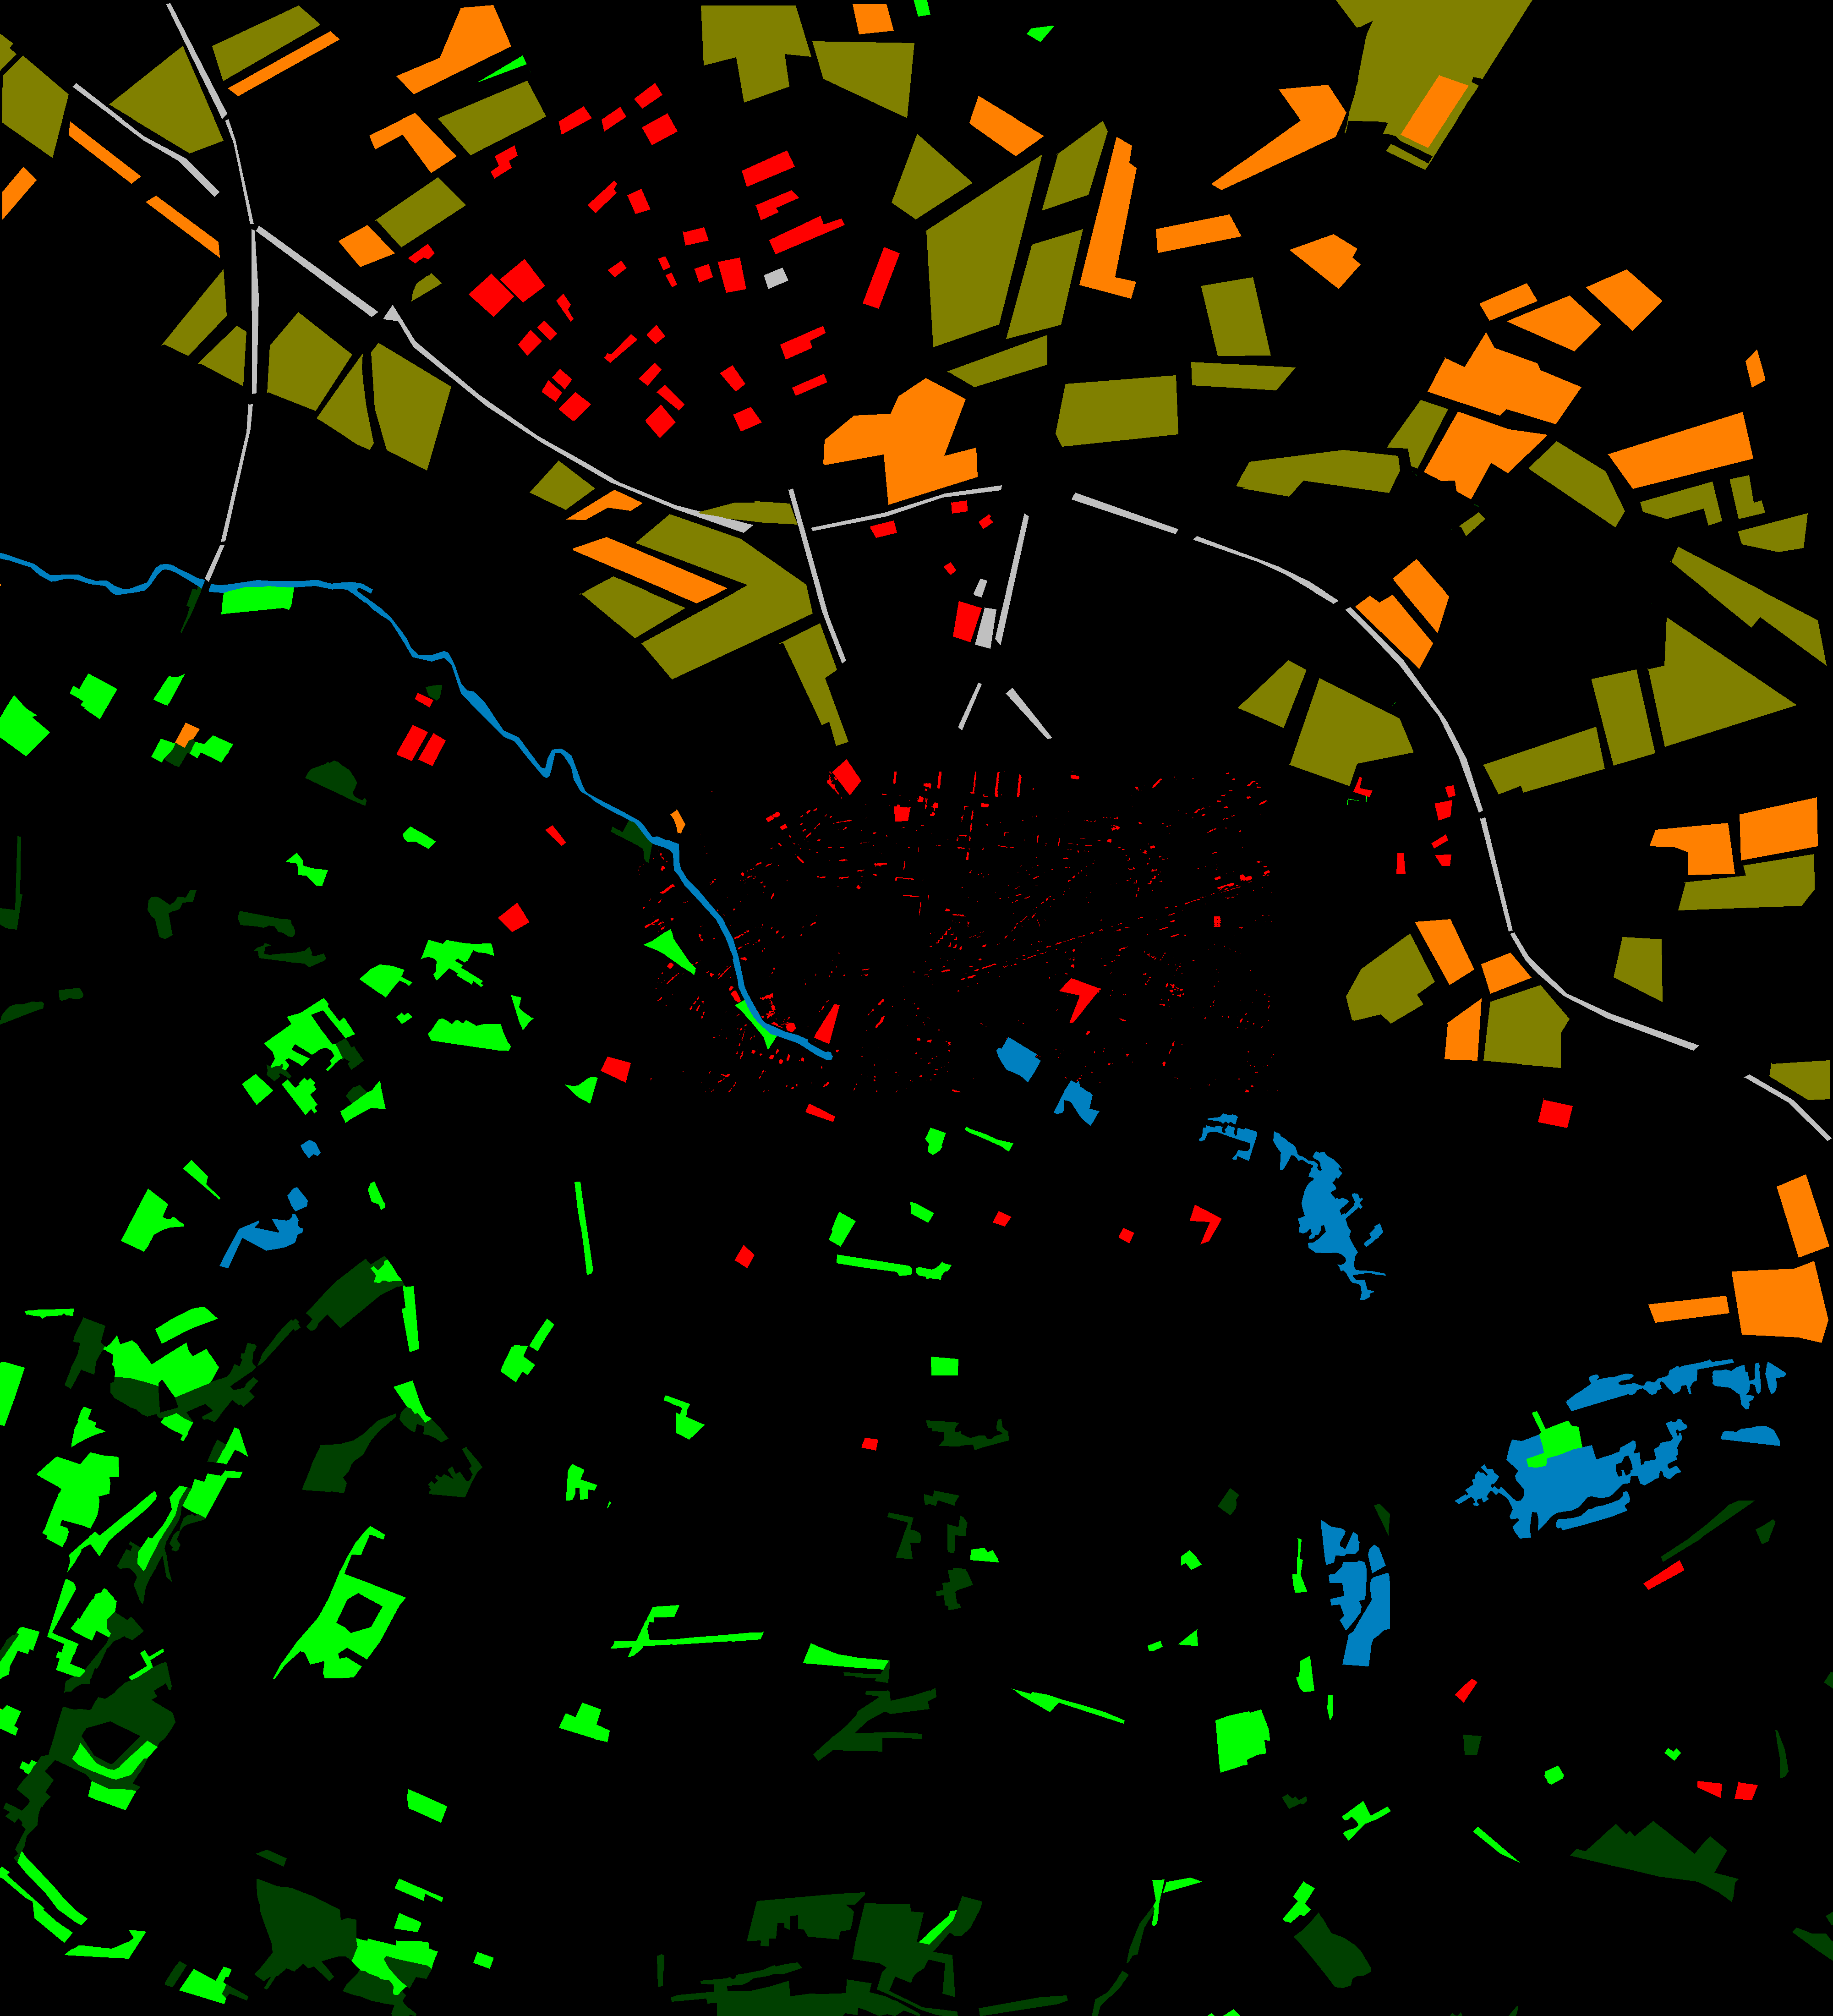
\includegraphics[width=0.4\textwidth]{GT_Amiens2006_2_5m_7classes_TR}}
     \hspace{4mm}
    \subfigure[Legenda classi della mappa di \emph{training}]{
      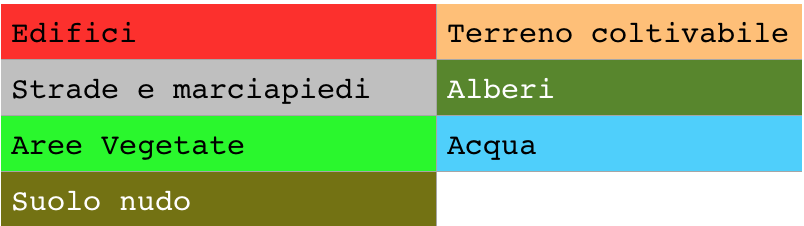
\includegraphics[scale=0.5]{Leggenda_7classi}}
    \caption{\emph{Dataset} con composizione RBG in falso colore ($4001\times4400$ pixel) acquisita su Amiens (Francia) dal sensore \textsc{SPOT5 HRG} nel 2006}
    \label{fig: Amiens62_5m}
  \end{figure}
\clearpage


\subsection{Amiens 2012 - 2.5m - 7 classi}
L'immagine \emph{Amiens12--2.5m} è stata acquisita nel 2012 e ha pixel di dimensione spaziale pari a $2.5\text{ }m$, coprendo sempre un'area di circa $10\text{ }km\times11\text{ }km$ ($4001\times4400$ pixel).\\
L'insieme delle classi $\Omega=\left\lbrace\omega_1,\omega_2,\ldots,\omega_{7}\right\rbrace$, che costituisce il \emph{dataset}, è lo stesso del precedente. Per uniformità vengono ugualmente riportate:
\begin{enumerate}
\item Edifici
\item Strade e marciapiedi
\item Aree vegetate
\item Suolo nudo
\item Terreno coltivabile
\item Alberi
\item Acqua
\end{enumerate}
Nella Figura \ref{fig: Amiens122_5m} vengono presentate le immagini caratterizzanti il primo \emph{dataset}; si osservi con attenzione la composizione dell'immagine di \emph{training}.\\
Anche in questo caso si nota come l'immagine a 2.5 m sia sfocata, rendendo il processo di classificazione largamente complesso. Infatti, la risoluzione spaziale di tale immagine è da ritenersi peggiore di 2.5 m, sempre a causa della parziale efficacia del metodo di super-risoluzione applicato in fase di pre-elaborazione.

\begin{lstlisting}[float=b,title={Distribuzione dei pixel di training(TR) e test(TE) classe per classe.},
                   label=lst:esempio, frame=lines]
TR:					TE:
Class 1: 132005				Class 1: 60793
Class 2: 76330				Class 2: 40123
Class 3: 351949				Class 3: 282545
Class 4: 933512				Class 4: 461562
Class 5: 451999				Class 5: 194213
Class 6: 363058				Class 6: 203286
Class 7: 170921				Class 7: 123744
Total  : 2479774			Total  : 1366266
\end{lstlisting}
\clearpage

\begin{figure}[!ht]
   \center
   \subfigure[Immagine telerilevata]{
      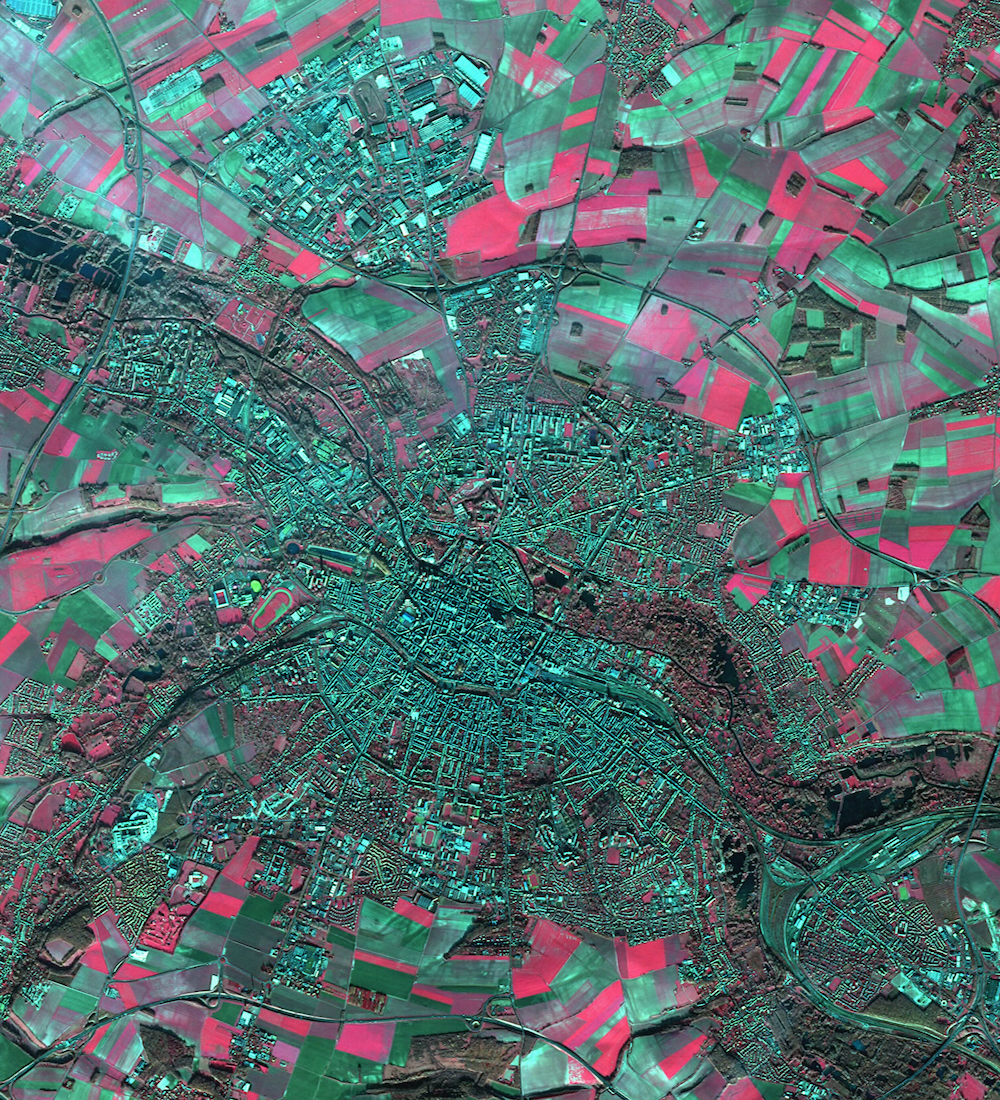
\includegraphics[width=0.7\textwidth]{Amiens_2012_SPOT_2_5m}}\\%pdf0.45
         \subfigure[Mappa di \emph{training}]{
      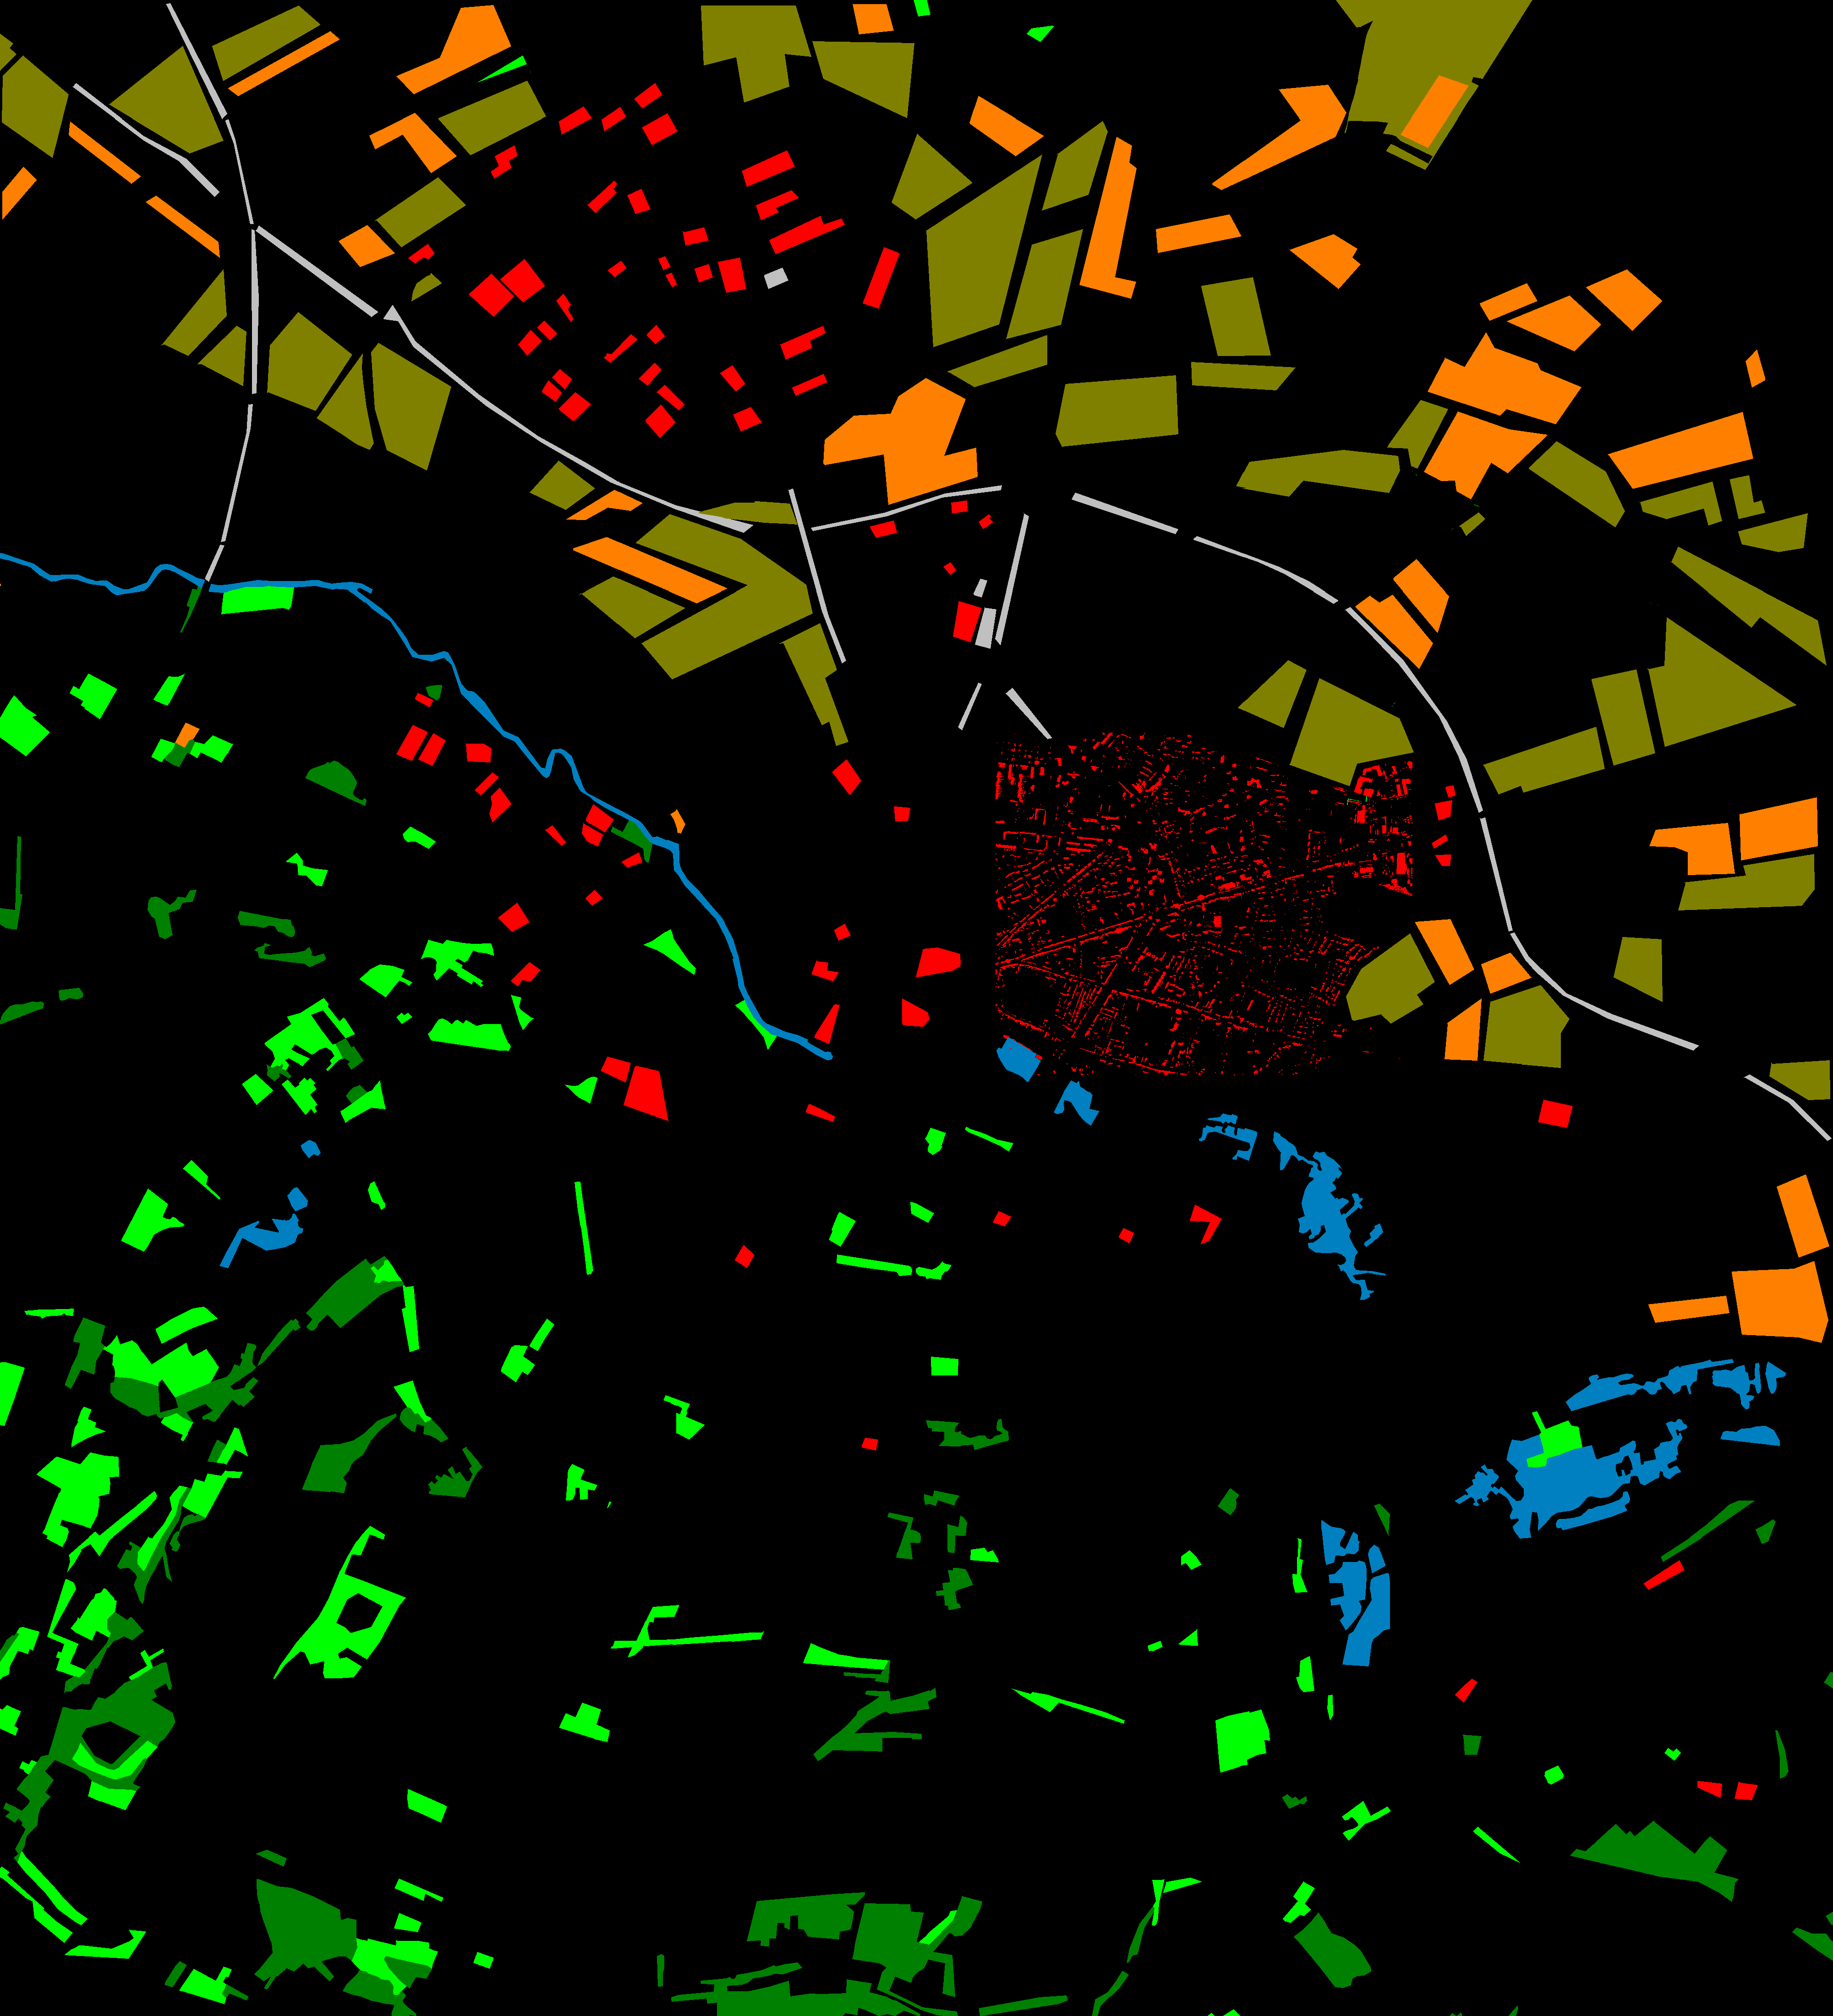
\includegraphics[width=0.4\textwidth]{GT_Amiens2012_2_5m_7classes_TR}}
     \hspace{4mm}
    \subfigure[Legenda classi della mappa di \emph{training}]{
      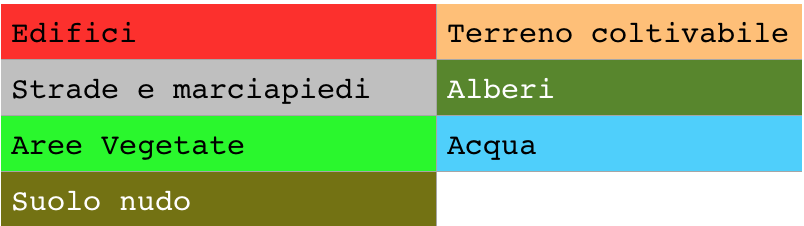
\includegraphics[scale=0.5]{Leggenda_7classi}}
    \caption{\emph{Dataset} con composizione RBG in falso colore ($4001\times4400$ pixel) acquisita su Amiens (Francia) dal sensore \textsc{SPOT5 HRG} nel 2012}
    \label{fig: Amiens122_5m}
  \end{figure}
\clearpage

\section{Applicazione del classificatore SVM}
Il classificatore usato è un classificatore \emph{soft-margin} SVM con \emph{kernel} gaussiano. L'implementazione adottata è una variante \emph{ad hoc} della \texttt{LIBSVM} [RIF] scritta in \texttt{C++}.\\
Il setup utilizzato per la fase di classificazione è composto da un \texttt{MacBookPro Retina} con un processore dual core Intel Core i5 $2.8$ GHz e $16$ GB di memoria e un \texttt{iMac} con processore quad core Intel Core i7 $3.4$ GHz e $8$ GB di memoria. \\

La fase di \emph{training} della SVM, la quale ha complessità temporale $O(n^\alpha)$ ($\alpha$ tipicamente compreso tra 2 e 3) polinomialmente proporzionale al numero di vettori di \emph{training}, ha impiegato, in media, 30 minuti per completare l'ottimizzazione dei parametri, mentre la fase di etichettatura (con complessità $O(n)$ dove $n$ è il numero di vettori da etichettare) ha impiegato, in media, un'ora per esperimento.\\
L'ottimizzazione dei parametri C e sigma del classificatore è stata effettuata mediante l'applicazione del metodo in [REF] che minimizza un maggiorante sull'errore di generalizzazione del classificatore, detto \emph{"span bound"}, mediante l'algoritmo numerico di Powell (per approfondimenti si faccia riferimento a \citep{art_ottsvm1} e \citep{art_ottsvm2}).


%

\section{Applicazione del metodo HOG}
Qui di seguito verranno presentate le variazioni di accuratezza dell'algoritmo sviluppato al variare delle diverse combinazioni dei parametri in gioco, evidenziando le motivazioni alla base delle scelte progettuali effettuate. La calibrazione dei parametri è stata effettuata sul \emph{dataset} di Amiens 2006-5m\ref{fig: Amiens65m}. 

\subsection{Riduzione del rumore}
La riduzione del rumore è stata effettuata, come già illustrato in figura \ref{fig:immagine_rumore} nel Capitolo \ref{cap:hog}, tramite un filtraggio passa-basso attraverso un filtro gaussiano bi-dimensionale avente varianza $\sigma$ pari a 2 pixel. Applicando questa gaussiana sia sull'immagine in ingresso all'algoritmo HOG sia sulle immagini HOG risultanti, si opera al fine di ottenere un notevole incremento nella \emph{average accuracy}. In particolare, l'utilizzo di un filtro gaussiano in ingresso aumenta l'AA del $12\%$, mentre l'algoritmo di \emph{noise cleaning} applicato prima e dopo l'estrazione delle \emph{feature} ha fatto registrare un'ulteriore incremento di 2 punti percentuali, portanto l'AA al $14\%$.

\subsection{Calcolo dei gradienti}
Per quanto riguarda la scelta della maschera da utilizzare per il calcolo del gradiente, sono state valutate diverse opzioni, tra cui la semplice maschera in $1D$ a differenze separate $[-1, 0 ,1]$, la maschera cubica $[1,-8,0,8,-1]$ e filtri  $2D$ più classici come quelli di Prewitt e Sobel.\\
I risultati migliori sono stati ottenuti con il \emph{kernel} più semplice a $1D$ $3\times1$. Variazioni sulla maschera utilizzata non hanno modificato significativamente i risultati per giustificare un aumento computazionale dovuto all'utilizzo di filtri più complessi.In particolare, con la maschera cubica $5\times5$ l'incremento della AA è stato di appena $+1,5\%$; negli altri casi valutati il risultato è sempre stato peggiore ($-7\%$ con Prewitt e $-3\%con Sobel$.Per questo motivo abbiamo deciso di utilizzare in tutti e tre i casi la soluzione più semplice e ottimale.\\

La direzione del gradiente è stata considerata tra $0$ e $\pi$ (ignorandone quindi il segno) in quanto le strutture geometriche di cui ci interessa avere informazioni (quali strade, fiumi, \ldots) possono essere identificate dalla direzione e non è invece rilevante il verso del gradiente.

\subsection{Numero di componenti dei vettori delle \emph{feature}}
Per quanto riguarda il numero di canali utilizzati per l'istogramma, la scelta che ha fornito prestazioni migliori è risultata essere quella con numero di bande pari a 4. Quantitativamente parlando, i risultati ottenuti con $9$\emph{orientation bins} hanno portato ad un decremento nella AA di $-11\%$. Inoltre, un aumento del numero di \emph{bins} comporta un aumento della risoluzione angolare e, pur apportando complessivamente poca informazione aggiuntiva,  aumenta la dimesionalità dello spazio delle \emph{feature} $\mathbb{R}^d$. Infatti, in primo luogo, all'aumentare di $d$, cresce la complessità computazionale del classificatore, che si traduce in un allungamento dei tempi di calcolo e in una maggiore occupazione di memoria.

\subsection{Dimensione delle celle e dei blocchi}
La scelta di utilizzare celle di elevate dimensioni introduce un'alta correlazione tra i vettori delle \emph{feature}, mentre un' eccessiva riduzione \textbf{comporta l'inserimento di vettori così scorrelati da avere valori praticamente associabili a rumore.} Un compromesso  è stata trovato empiricamente attraverso diverse sperimentazioni ed è risultato essere diverso (come ci si può aspettare) a seconda della risoluzione spaziale con cui si operava:
\begin{itemize}
\item cella da $4\times 4$ pixel, nel caso di pixel di dimensione spaziale pari a 5 m (Figure \ref{fig: Amiens65m})
\item cella da $2 \times 2$ pixel, nel caso di pixel di dimensione spaziale pari a 2.5 m (Figure \ref{fig: Amiens62_5m} e \ref{fig: Amiens122_5m})
\end{itemize}

Si è deciso di mantenere costante il numero di pixel usati per la normalizzazione dei blocchi ad un valore di $16\times16$, dal momento che questo valore non inficia la quantità di informazione a disposizione, ma semplicemente normalizza i valori gia calcolati, limitandone l'escursione entro un certo intervallo predefinito.

\clearpage

\section{Discussione dei risultati sperimentali}

\subsection{Amiens 2006 - 5m - 10 classi}

\'E riportata in Figura \ref{fig:ClassMap_Amiens2006_5m} la mappa di
classificazione con \emph{feature} HOG aggiuntive in configurazione di
$4$ \emph{bins}, celle di dimensione $4\times4$ pixel e blocchi di
normalizzazione con $16\times16$ pixel, con filtraggio gaussiano sia
per l'immagine in ingresso che per le immagini HOG.

\begin{figure}[!ht]
\center
\subfigure{
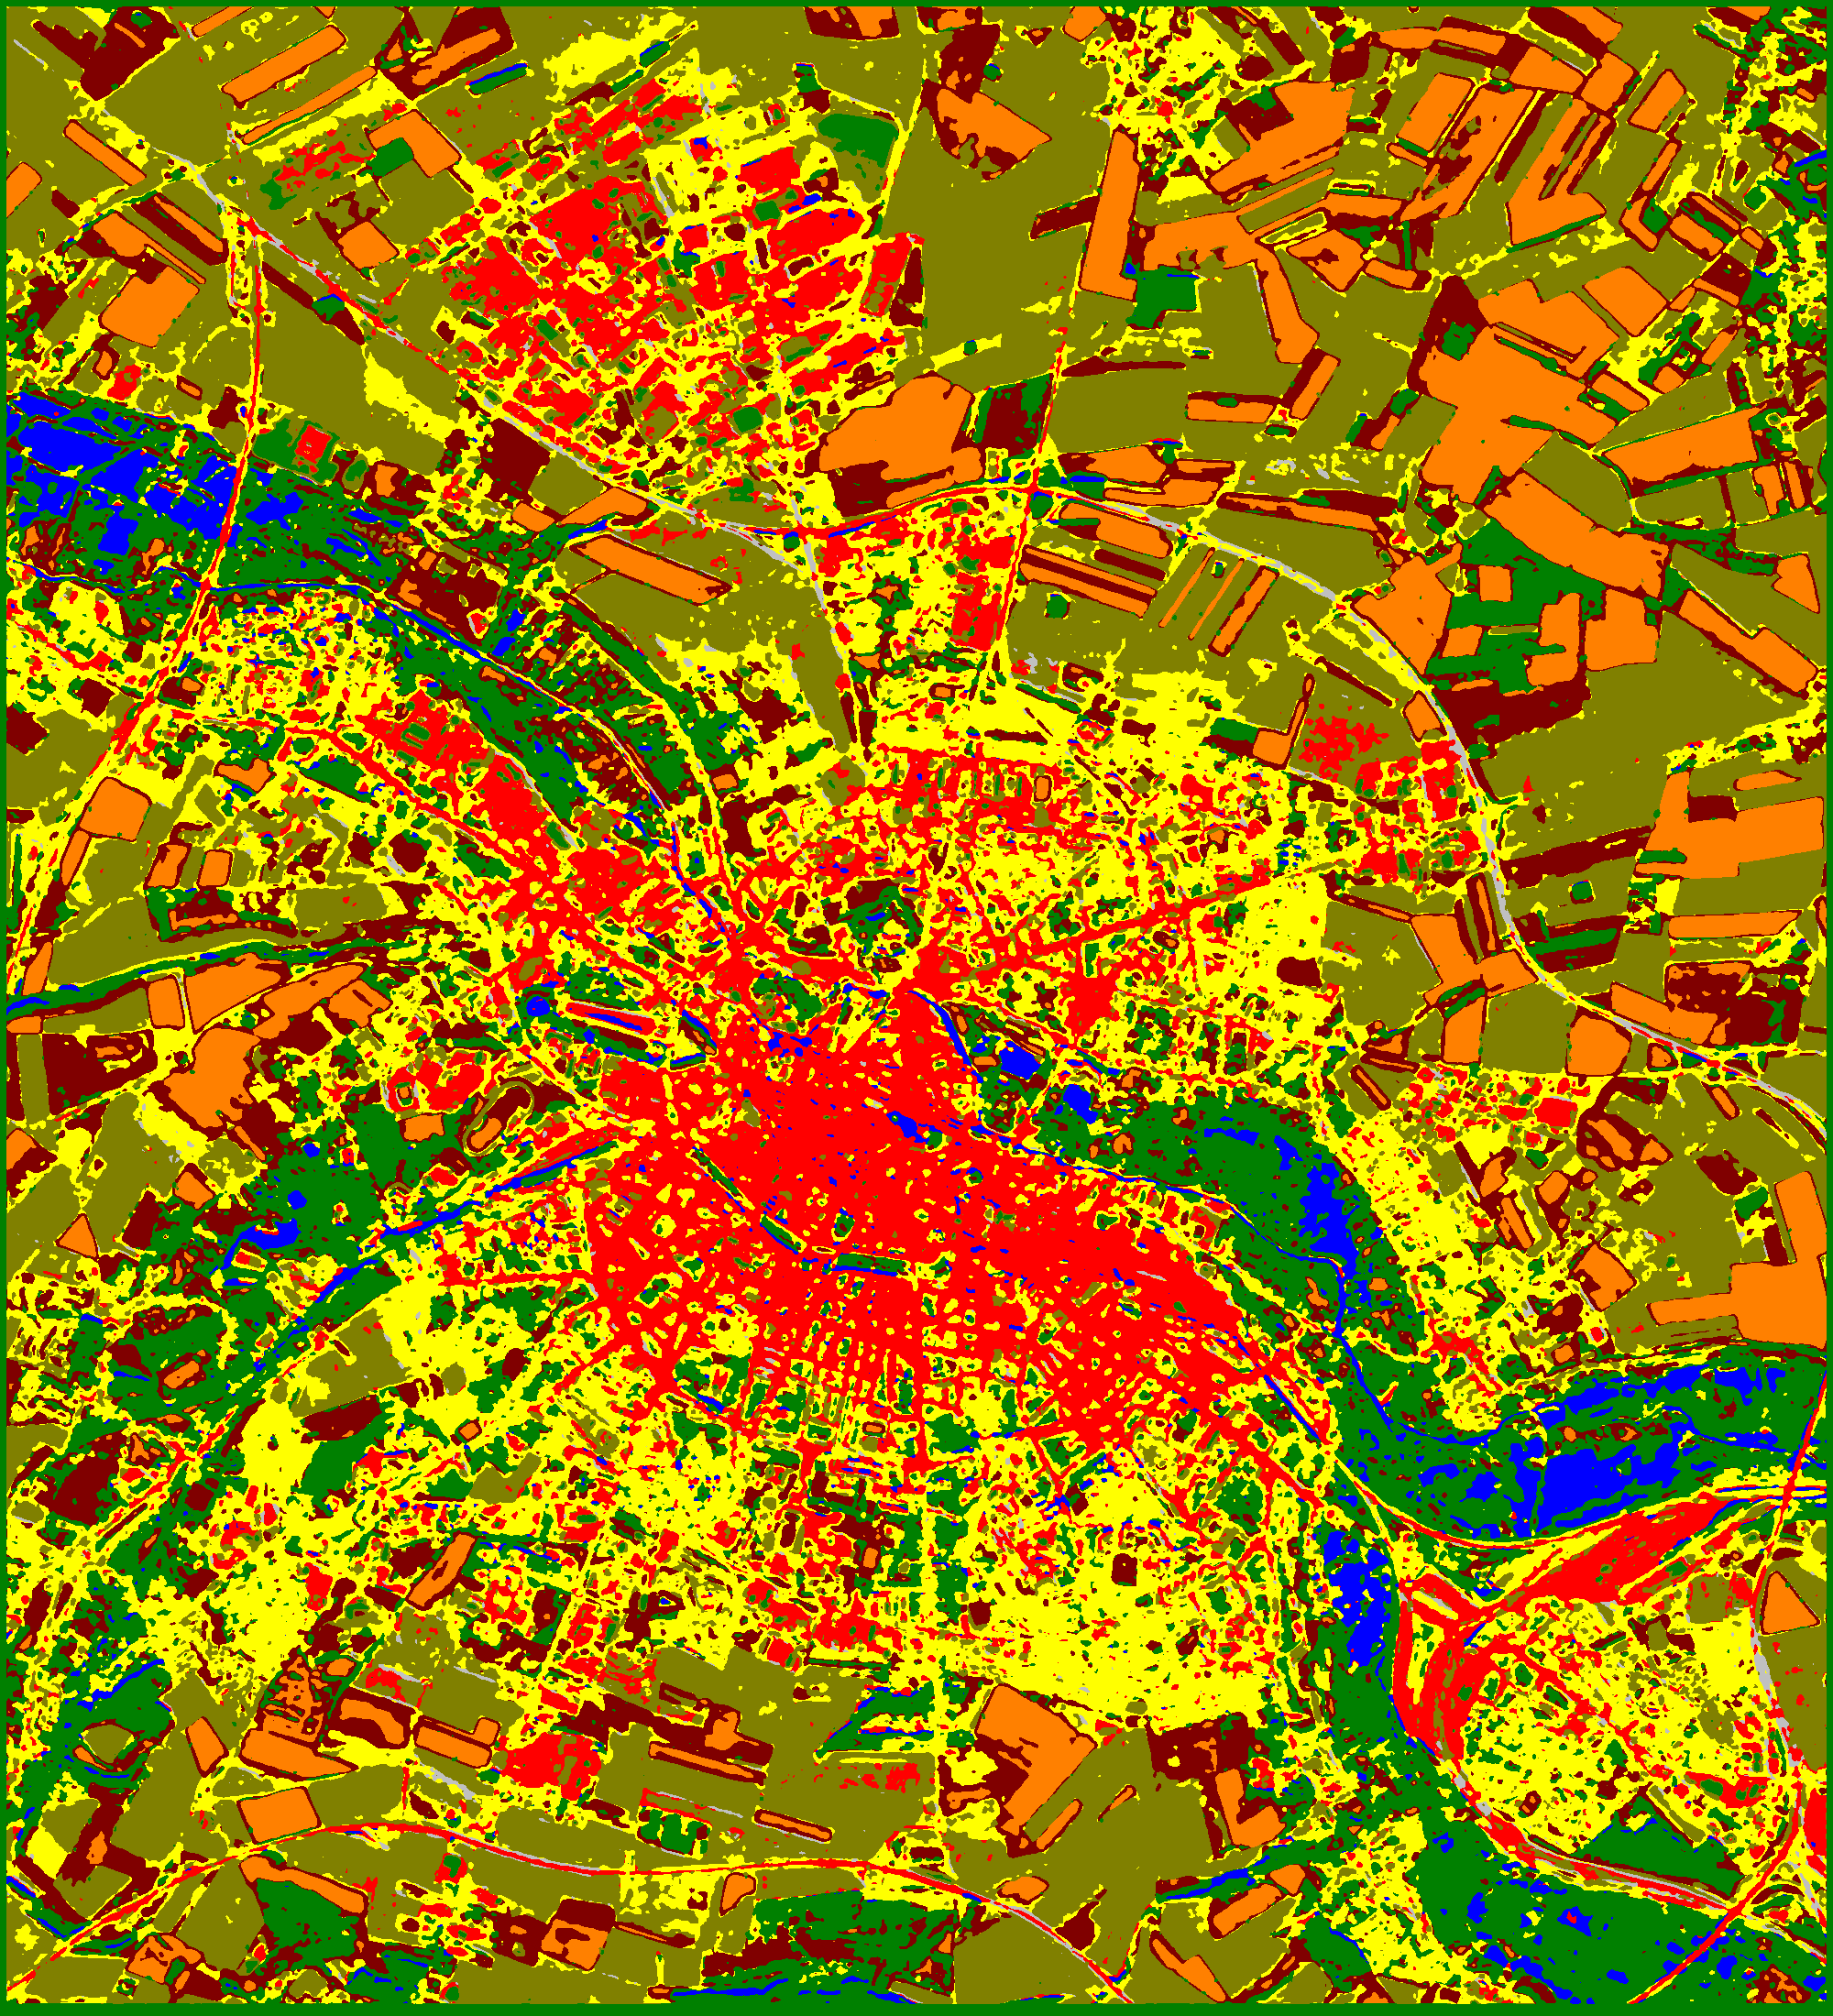
\includegraphics[width=0.7\textwidth]{ClassMap_Amiens2006_5m}}
\\
\subfigure{
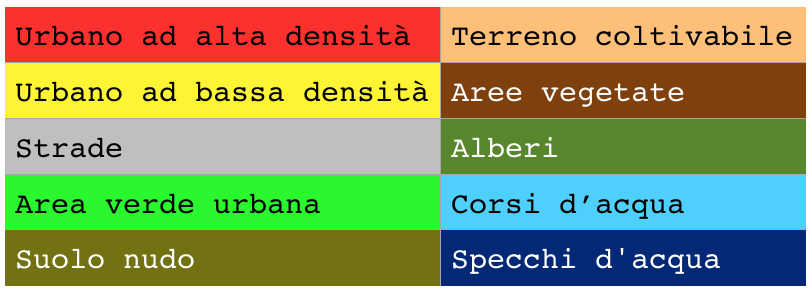
\includegraphics[width=0.35\textwidth]{Leggenda_2006_10classi}}

\caption{Mappa di classificazione ottenuta applicando SVM a feature spettrali e HOG per il \emph{dataset} \emph{Amiens 2006 - 5m - 10 classi}}

\label{fig:ClassMap_Amiens2006_5m}

\end{figure}
\clearpage
Da una prima analisi visiva, si può chiaramente constatare come nel
complesso la mappa di classificazione sia soddisfacente, sebbene si
noti già adesso difficoltà nella classificazione delle strade (classe
3) soprattutto all'interno dell'area urbana. Inoltre, è evidente che
la classe relativa ai corsi d'acqua (classe 9) non è presente (o
almeno non apprezzabile).

Sono stati evidenziati, principalmente, due problemi:
\begin{itemize}
\item Il primo problema è legato alla risoluzione spaziale dell'immagine in
ingresso che permette l'identificazione di strade abbstanza larghe, ma
rende difficoltosa l'identificazione di strade più strette.
\item Il secondo problema si correla col fatto che il \emph{dataset} include due classi
associate a corpi idrici: pur rappresentando essi usi del suolo
differenti, le loro coperture del suolo sono effettivamente analoghe,
il che ne rende difficile la discriminazione mediante dati
satellitari, soprattutto caartterizzati da pochi canali spettrali
(solo tre nel nostro caso).
\end{itemize}

Queste prime impressioni vengono confermate anche dall'analisi numerica della matrice di confusione (Figura
\ref{fig:Matrice_di_confusione_Amiens2006_5m_HOG}).

\begin{figure}[!ht]

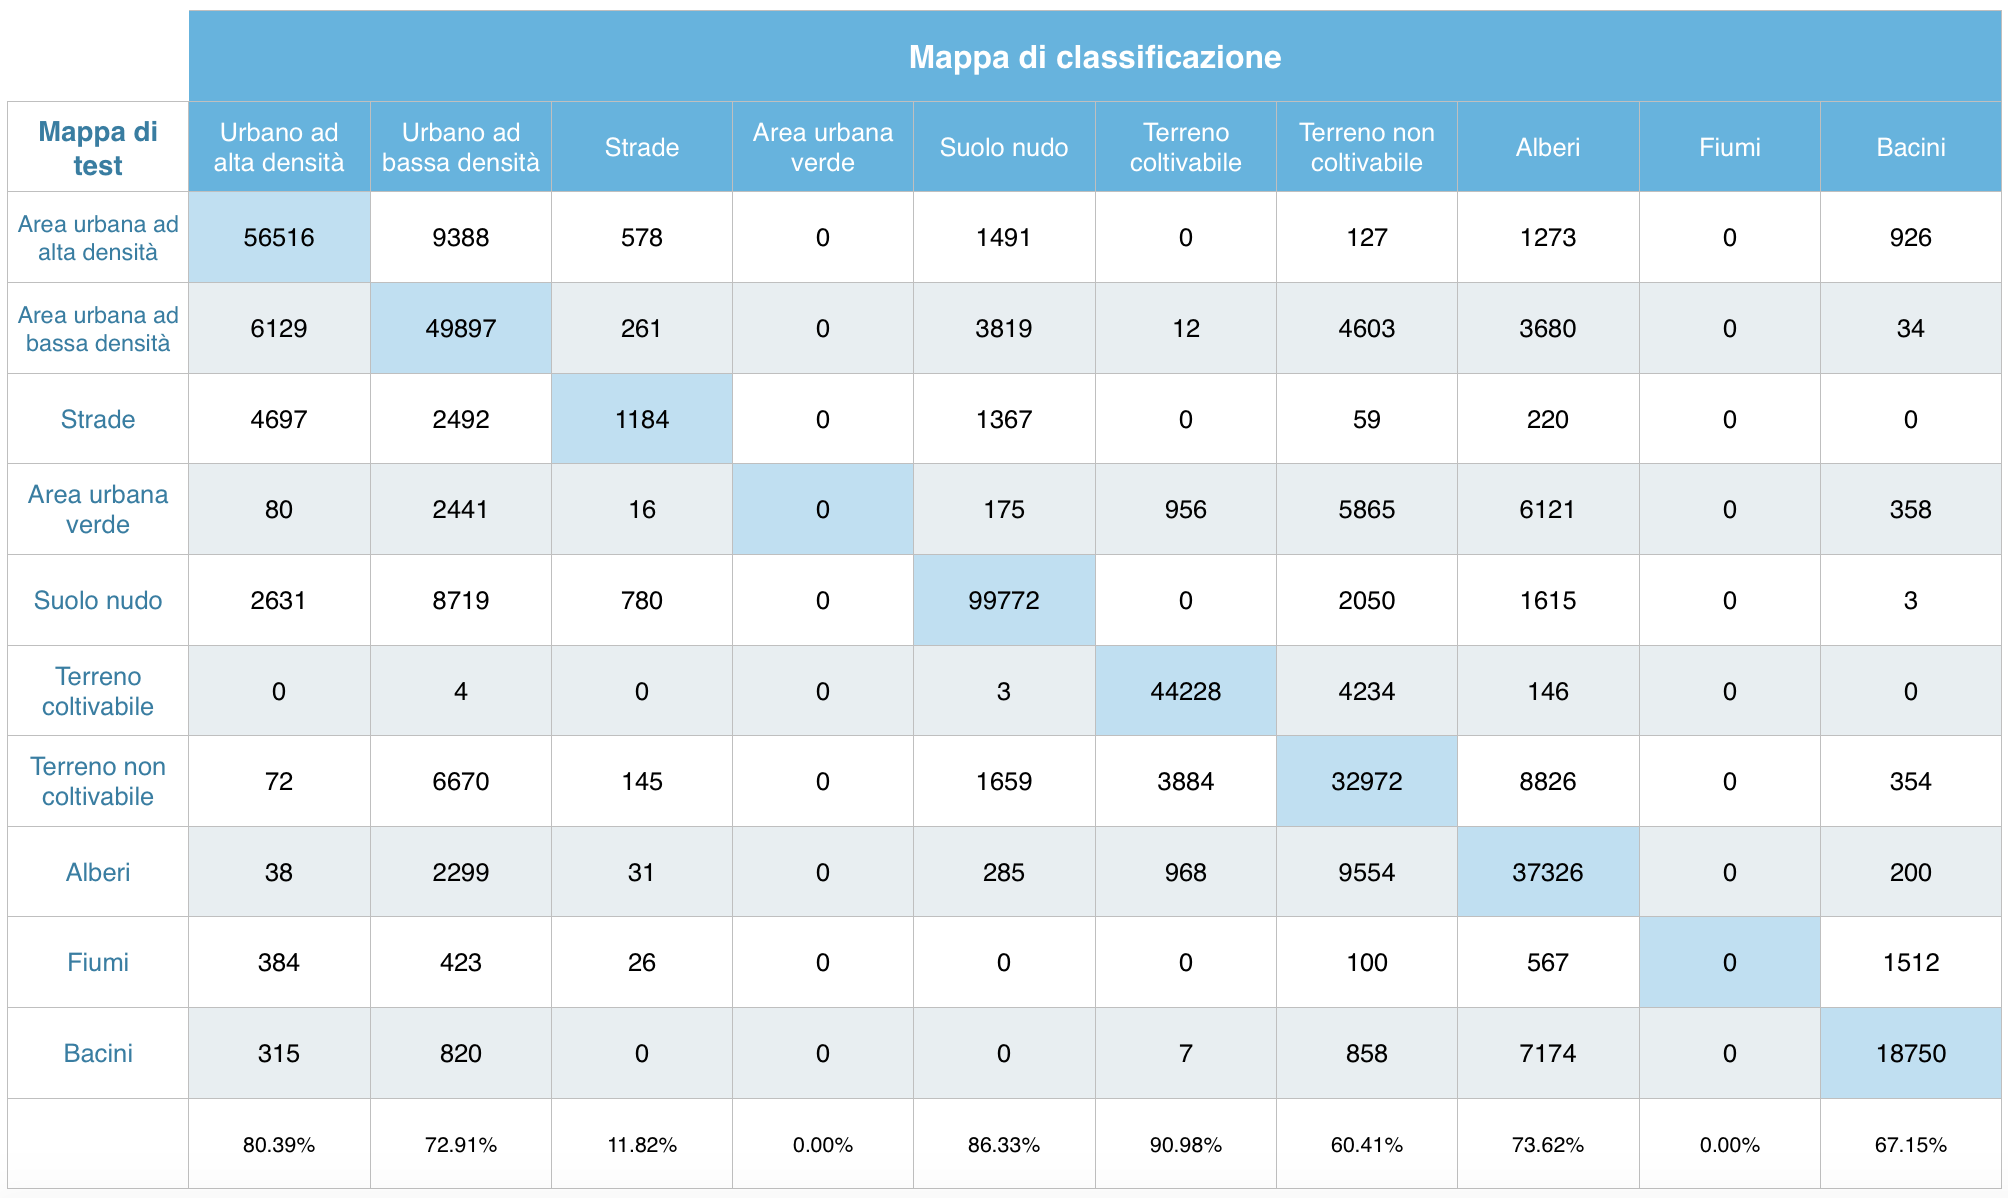
\includegraphics[width=1\textwidth]{Matrice_di_confusione_Amiens2006_5m_HOG}

\caption{Matrice di confusione associata alla classificazione del
dataset \emph{Amiens 2006 - 5m - 10 classi} mediante l'applicazione di SVM a feature spettrali e HOG}

\label{fig:Matrice_di_confusione_Amiens2006_5m_HOG}

\end{figure}

Analizzando la matrice di confusione saltano subito all'occhio alcuni
comportamenti interessanti nella classificazione. La zona urbana
(classe 1 e 2) viene discriminata in modo soddisfacente (con
accuratezze nell'ordine del $75\%$); ciò che si perde nell'accuratezza
deriva in massima parte dalla difficoltà del classificatore di
distinguere le aree urbane di diversa densità.\\

L'analisi quantitativa della matrice di confusione conferma quanto già
ipotizzato precedentemente, ovvero che le strade sono quasi del tutto
perse registrando un'accuratezza di circa $11\%$, a scapito sopratutto
dell'area urbana. \\

Si è registrata una buona accuratezza nelle classificazioni di aree
più uniformi quali suolo nudo (classe 5), terreni coltivabili e non
coltivabile (classi 6 e 7): pochissimi sono i pixel etichettati in
modo errato per queste regioni, analogamente ai terreni non
coltivabili, per i quali tuttavia la confusione con la classe "alberi"
causa accuratezza inferiore.\\

Tuttavia, il classificatore ha avuto serie difficoltà in quelle classi
minoritarie per le quali il numero di pixel di training era inferiore.
In particolare, vengono completamente perse l'area verde urbana e i
corsi d'acqua ($0\%$), le cui etichette sono state assegnate in
maggioranza alla classe alberi e alla classe bacini d'acqua,
rispettivamente.\\

Come osservato prima, si tratta di un errore di classificazione dovuto
alla difficoltà di distinguere classi associate a distinti usi del
suolo ma sostanzialmente a coperture del suolo molto simili. In
quest'ottica, il risultato ottenuto si ritiene già soddisfacente.\\

La difficoltà di classificazione di questo \emph{dataset} risiede
soprattutto nella sovrabbondanza del numero di classi da distinguere,
in quanto molti errori fatti nella mappa di classificazione sono
proprio causati dalla confusione di coperture di suolo simili tra
loro.\\

In termini generali, l'\emph{Overall Accuracy} (OA) complessivo di
questo primo \emph{dataset} è stato di $73.23\%$, mentre l'AA è
risultato essere $54.36\%$. Il più basso valore di AA è legato al
fatto che accuratezze più elevate si siano ottenute per classi
minoritarie in termini di pixel di test.\\

Per concludere questa prima sessione di discussione, è interessante
confrontare questi risultati con quelli ottenuti senza estrazione
delle \emph{feature} HOG. La Figura \ref{fig:Confronto_Amiens2006_5m}
sintetizza i miglioramenti/peggioramenti classe per classe.

\begin{figure}[!ht]

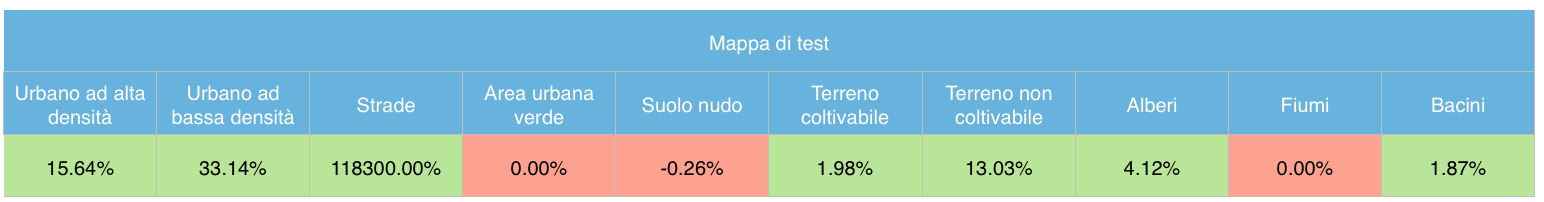
\includegraphics[width=1\textwidth]{Confronto_Amiens2006_5m}

\caption{Differenze tra le accuratezze classe per classe con e
senza estrazione di \emph{feature} HOG per il data set \emph{Amiens 2006 - 5m - 10 classi}}

\label{fig:Confronto_Amiens2006_5m}

\end{figure}

Si può chiaramente osservare che l'introduzione delle \emph{feature}
HOG ha quasi sempre apportato miglioramenti, con benefici notevoli
soprattutto per le classi di suolo urbano. La Figura
\ref{fig:Confronto_Amiens2006_5m} dimostra come effettivamente il
risultato della classificazione dell'immagine a tre canali mostri in
generale più dettaglio; così facendo, però, ciò che si guadagna in
risoluzione si perde in accuratezza nella classificazione, in quanto
molti pixel urbani vengono etichettati come appartenenti ad altre
classi (in particolare la classe 10, gli specchi d'acqua,
rappresentata in bianco nelle immagini). Il miglioramento ottenuto per
le classi urbane è coerente con l'informazione direzionale estratta
dalle feature HOG che risulta utile soprattutto ai fini della
discriminazione di classi caratterizzate da struttura geometrica.

\begin{figure}[!ht]

\center

\subfigure[Mappa di classificazione con HOG]{

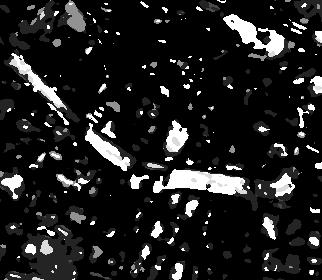
\includegraphics[width=0.4\textwidth]{ClassMap_Amiens2006_5m_HOG}}

\hspace{2mm}

\subfigure[Mappa di classificazione senza HOG]{

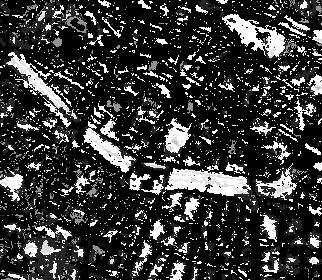
\includegraphics[width=0.4\textwidth]{ClassMap_Amiens2006_5m_riferimento}}

\caption{Confronto su una porzione dell'area urbana di $250\times250$
pixel della mappa di classificazione con e senza estrazione di
\emph{feature} HOG sul \emph{dataset} Amiens 2006 a $5$ m(il nero rappresenta gli "edifici", mentre i pixel bianchi corrispondono alla classe "acqua")}

\label{fig:confrontoAmiens2006_5m}

\end{figure}

\clearpage

%\subsection{Amiens 2006 - 2.5m - 7 classi}

%Come già introdotto nel caso precedente, anche per questo esperimento

%foto-interpretativa

%\clearpage

\subsection{Amiens 2012 - 2.5m - 7 classi}

\'E riportata in Figura \ref{fig:ClassMap_Amiens2012_2_5m_noroads} la
mappa di classificazione con \emph{feature} HOG, in aggiunta alle tre
feature spettrali, in configurazione di $4$ \emph{bins}, celle di
dimensione $2\times2$ pixel e blocchi di normalizzazione con
$16\times16$ pixel, con filtraggio gaussiano sia per l'immagine in
ingresso che per le immagini HOG.

\begin{figure}[!ht]

\center

\subfigure{

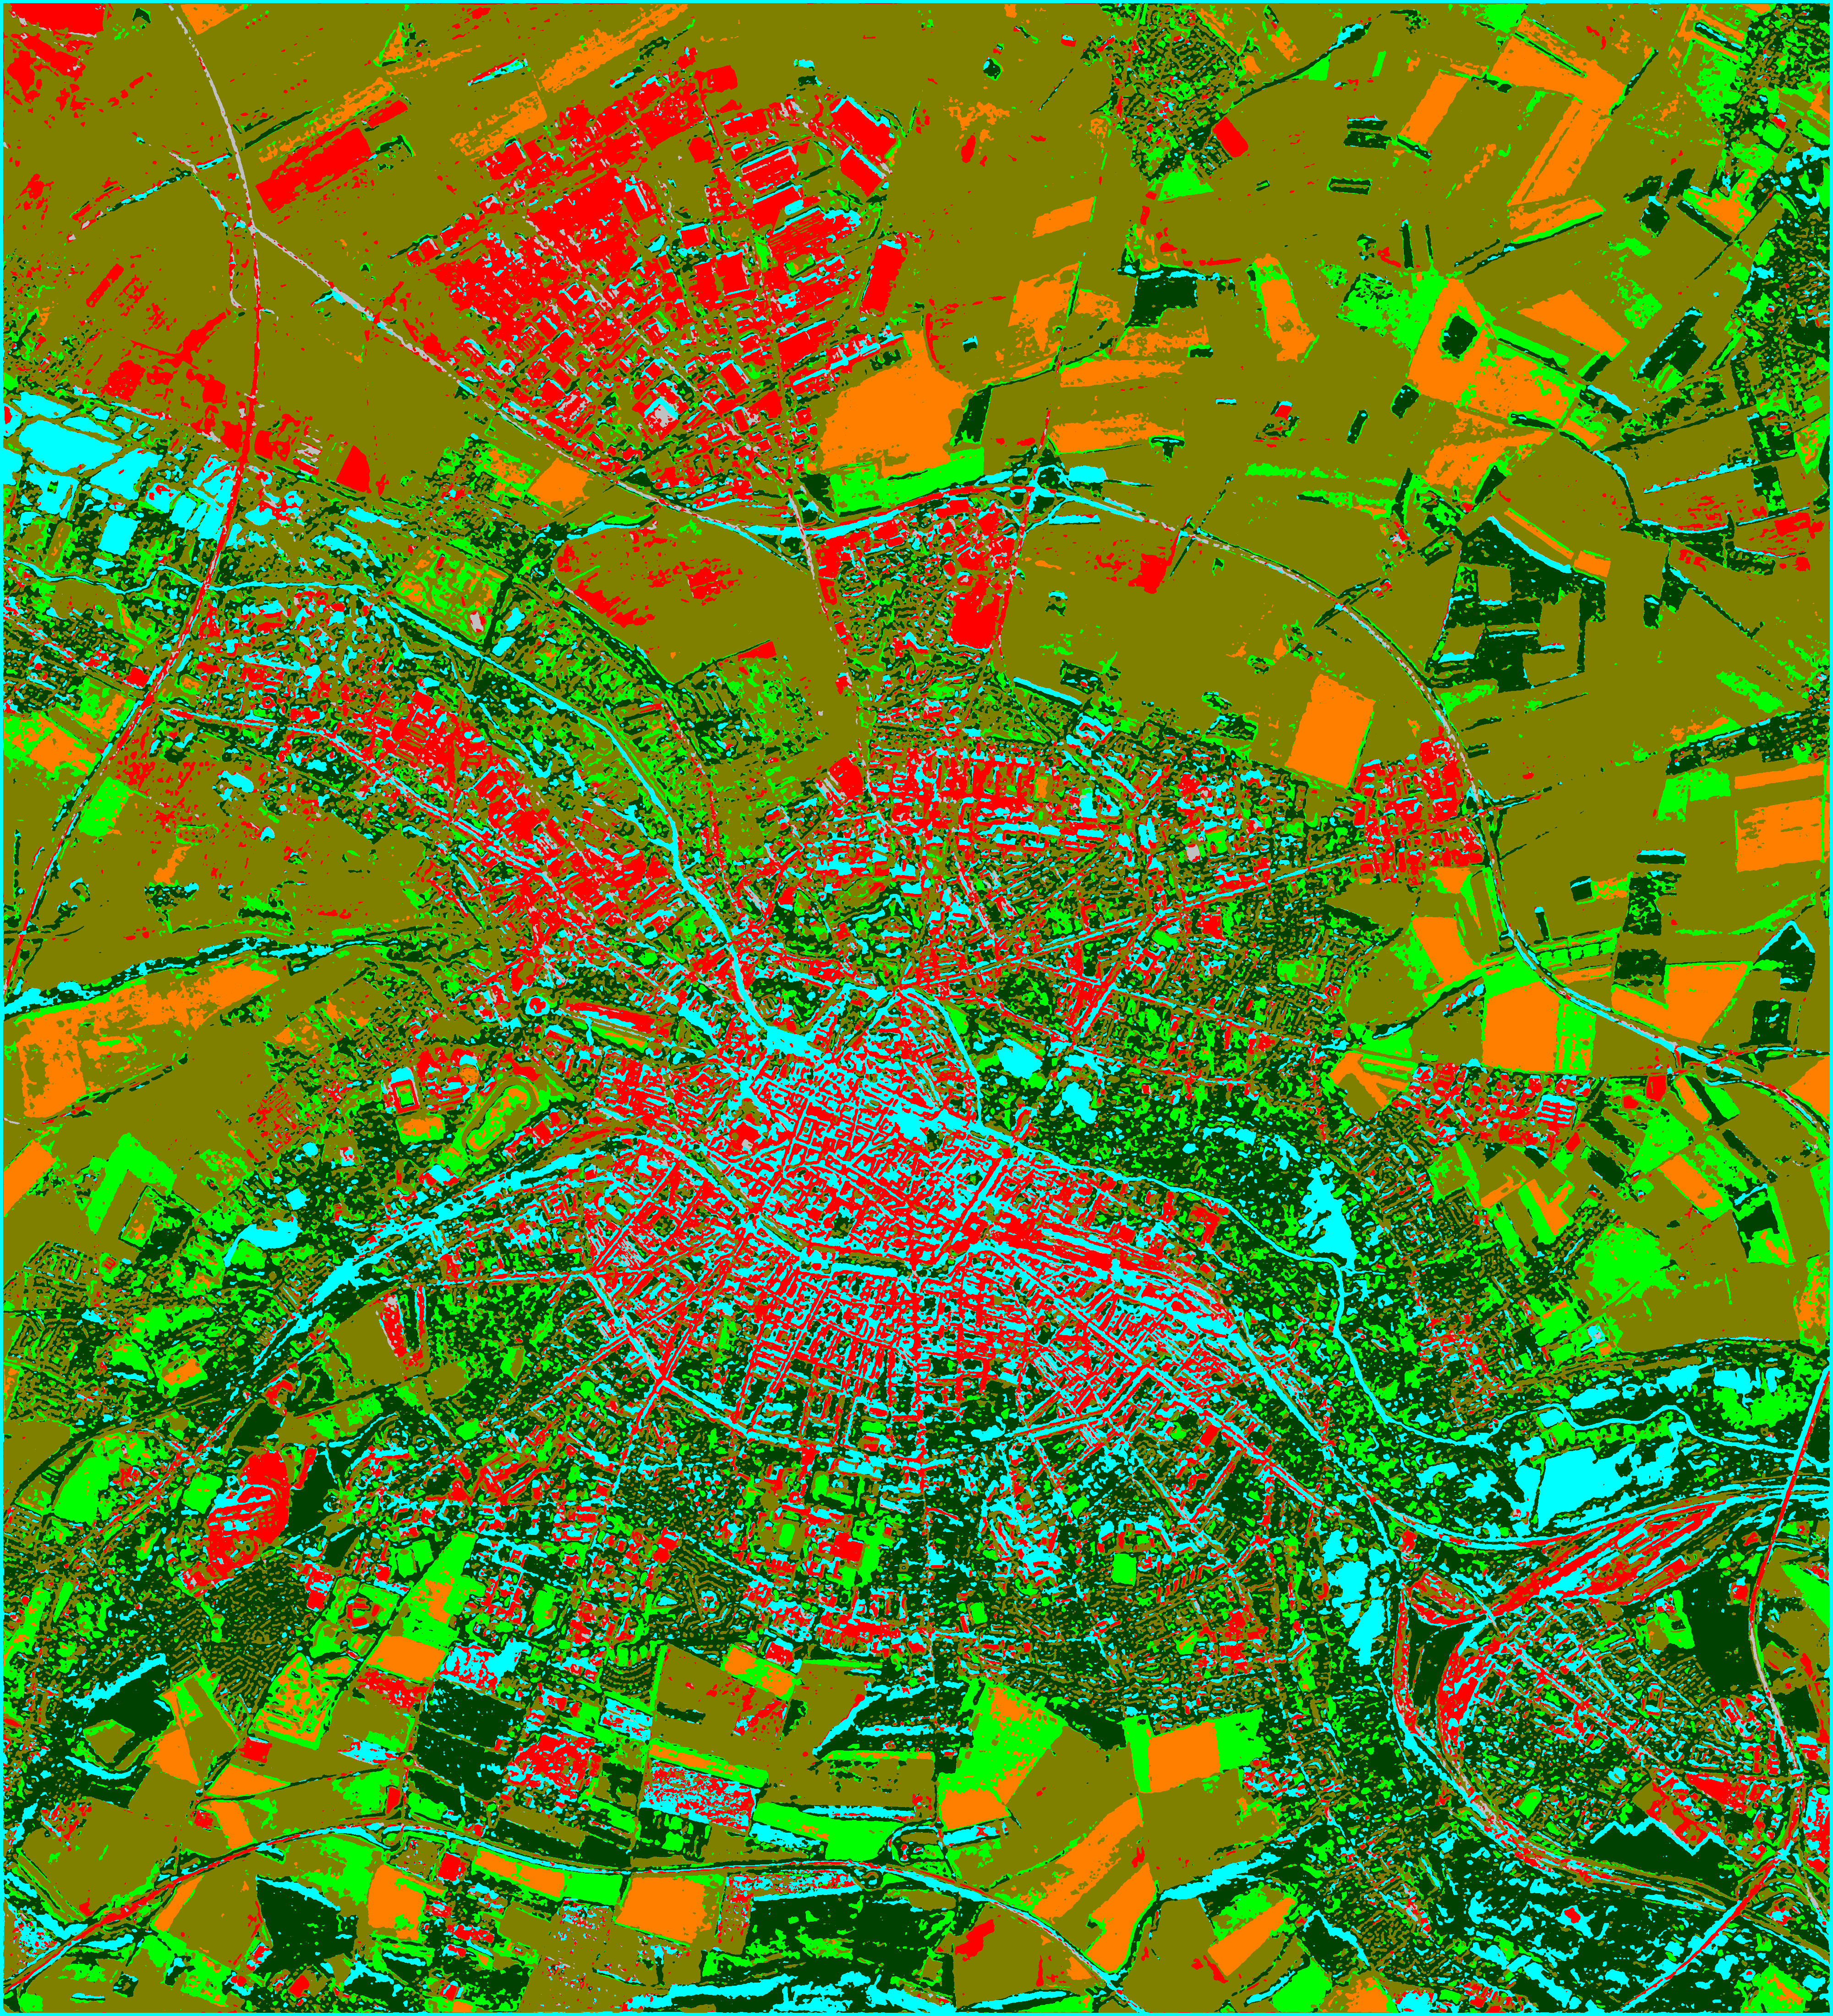
\includegraphics[width=0.7\textwidth]{ClassMap_Amiens2012_2_5m_noroads}}
\\
\subfigure{
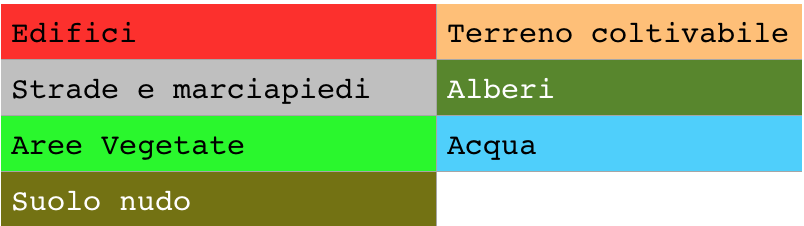
\includegraphics[width=0.35\textwidth]{Leggenda_7classi}}

\caption{Mappa di classificazione ottenuta applicando SVM a feature spettrali e HOG per il dataset \emph{Amiens 2012 - 2.5m
- 7 classi}}

\label{fig:ClassMap_Amiens2012_2_5m_noroads}

\end{figure}
\clearpage
\'E importante far notare fin da subito che l'immagine telerilevata
che fa parte di questo \emph{dataset} è stata acquisita in situazioni
ambientali e in periodi di tempo diversi da quelle precedenti
(nell'inverno 2012). Questo costituisce un evidente deficit
nell'informazione proveniente dal suolo, in quanto la stagione di
acquisizione ha reso altamente più complesso la discriminazione delle
7 diverse coperture di suolo. Le classi vegetate, in particolare,
corrispondono qui a coperture del suolo che presentano similarità col
suolo nudo, avendo l'acquisizione avuto luogo in un periodo dell'anno
in cui gli alberi avevano perso le foglie e le aree agricole non
presentavano gia più vegetazione coltivata evidente.\\

Già con un'analisi della mappa, si osserva che qualitativamente il
risultato sembra peggiorare rispetto all'esperimento precedente. Due
sono i punti critici già a prima vista apprezzabili:

\begin{itemize}

\item i pixel etichettati come appartenenti al suolo nudo (classe 4)
sembrano essere in misura sovrabbondante rispetto ai risultati precedenti: ciò
può essere giustificato dal commento precedente;

\item la quasi totale scomparsa delle strade (classe 2) nel centro,
che talora vengono classificate come pixel appartenenti alla classe
acqua (classe 7). Ciò si spiega non solo in relazione alla risoluzione
spaziale dell'immagine considerata ma anche col fatto che molte strade
presentino ombre di alcuni edifici; soprattutto quando osservata con
tre soli canali, la risposta spettrale delle zone in ombra si presenta
molto simile a quella dei corpi idrici.

\end{itemize}

Queste considerazioni trovano conferma negli indici di accuratezza che
raggiungono, in assoluto, valori meno soddisfacenti rispetto ai casi
esaminati in precedenza.

L'OA per questo esperimento, infatti, si è fermata al $56.63\%$,
mentre l'AA ha raggiunto il valore di $57.33\%$.\\

In Figura \ref{fig:Matrice_di_confusione_Amiens2012_5m_HOG_without_roads}
viene presentata la matrice di confusione di questo esperimento. \\

\begin{figure}[!ht]

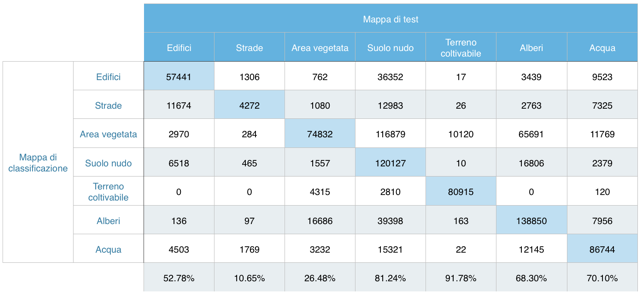
\includegraphics[width=1\textwidth]{Matrice_di_confusione_Amiens2012_5m_HOG_without_roads}

\caption{Matrice di confusione della sessione di classificazione del
\emph{dataset} \emph{Amiens 2012 - 5m - 7 classi}}

\label{fig:Matrice_di_confusione_Amiens2012_5m_HOG_without_roads}
\end{figure}

Si può osservare che la classe per la quale la classificazione ha
ottenuto i risultati migliori è stata quella relativa al terreno
coltivabile (classe 5), che ha registrato un accuratezza di oltre il $90\%$.
Prestazioni soddisfacenti sono state raggiunte anche per le classi di
suolo nudo e acqua (classi 4 e 7), in cui una buona percentuale di
pixel della mappa di classificazione coincide con la verità al
suolo.\\

% \begin{figure}[!ht]
%
%\center
%
% \subfigure[Mappa di classificazione senza HOG]{
%
% 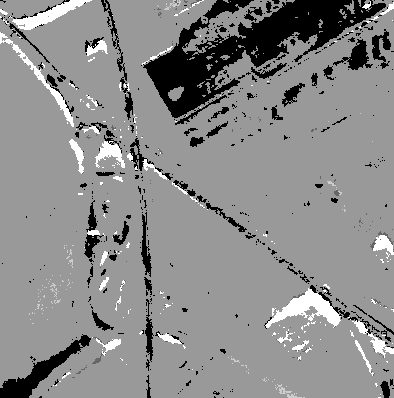
\includegraphics[width=0.4\textwidth]{ClassMap_Amiens2012_2_5m_riferimento}
%
% }
%
% \hspace{3mm}
%
% \subfigure[Mappa di classificazione con HOG]{
%
% 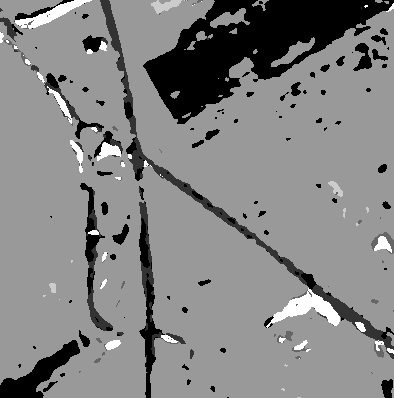
\includegraphics[width=0.4\textwidth]{ClassMap_Amiens2012_2_5m_HOG}
% } \caption{Confronto su una porzione dell'area urbana di
%$250\times250$ pixel della mappa di classificazione con e senza
%estrazione di \emph{feature} HOG sul \emph{dataset} Amiens 2012 a
%$2.5$ m }
% \label{fig:confrontoAmiens2012_2_5m}
%\end{figure}

\begin{figure}[!ht]

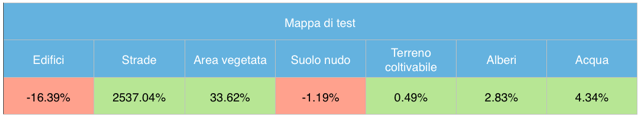
\includegraphics[width=1\textwidth]{Confronto_Amiens2012_con_e_senza_hog}

\caption{Differenze tra le accuratezze classe per classe con e
senza estrazione di \emph{feature} per il \emph{dataset} Amiens 2012 a
$2.5$ m}

\label{fig:Confronto_Amiens2012_2.5m}

\end{figure}

Confrontando i risultati ottenuti dalla classificazione con HOG e da
quella avente come \emph{feature} le sole tre bande telerilevate, si
osserva come, anche questa volta, l'introduzione degli HOG porti, in
generale, ad un incremento della percentuale di pixel classificati
correttamente: in particolare in Figura
\ref{fig:Confronto_Amiens2012_2.5m} si può notare un netto
miglioramento ($+2537\%$) per le strade, benché in termini assoluti
restino ancora ben poco classificate ($10\%$) probabilmente a causa
della presenza di ombre . Si è rilevato, tuttavia, un leggero
peggioramento ($-16\%$) nell' individuazione degli edifici. \\ In
conclusione, la presenza degli HOG migliora anche OA e AA seppure in
maniera limitata. \\

Vista la non ancora soddisfacente percentuale di pixel di strada
classificati in maniera adeguata, si è deciso di inserire una
\emph{feature} aggiuntiva della struttura cartografica delle strade di
Amiens. L'immagine binaria in Figura \ref{fig:immagine_roads} è stata
inserita nel vettore delle \emph{feature} in coda all'immagine
precedente con vettori HOG.

Quest'immagine è il risultato della fusione di tre mappe tematiche
(strade principali, strade secondarie e binari ferroviari, riportati
unitamente a parte del territorio circostante quando tale territorio
non presenti altro uso che quello associato ai trasporti), ottenuta
dal servizio di mappatura stradale della European Urban Atlas. In
particolare, l'immagine è aggiornata all'anno $2006$ e possiede una
risoluzione spaziale di 5 m/pixel.

\begin{figure}[!ht]
\center
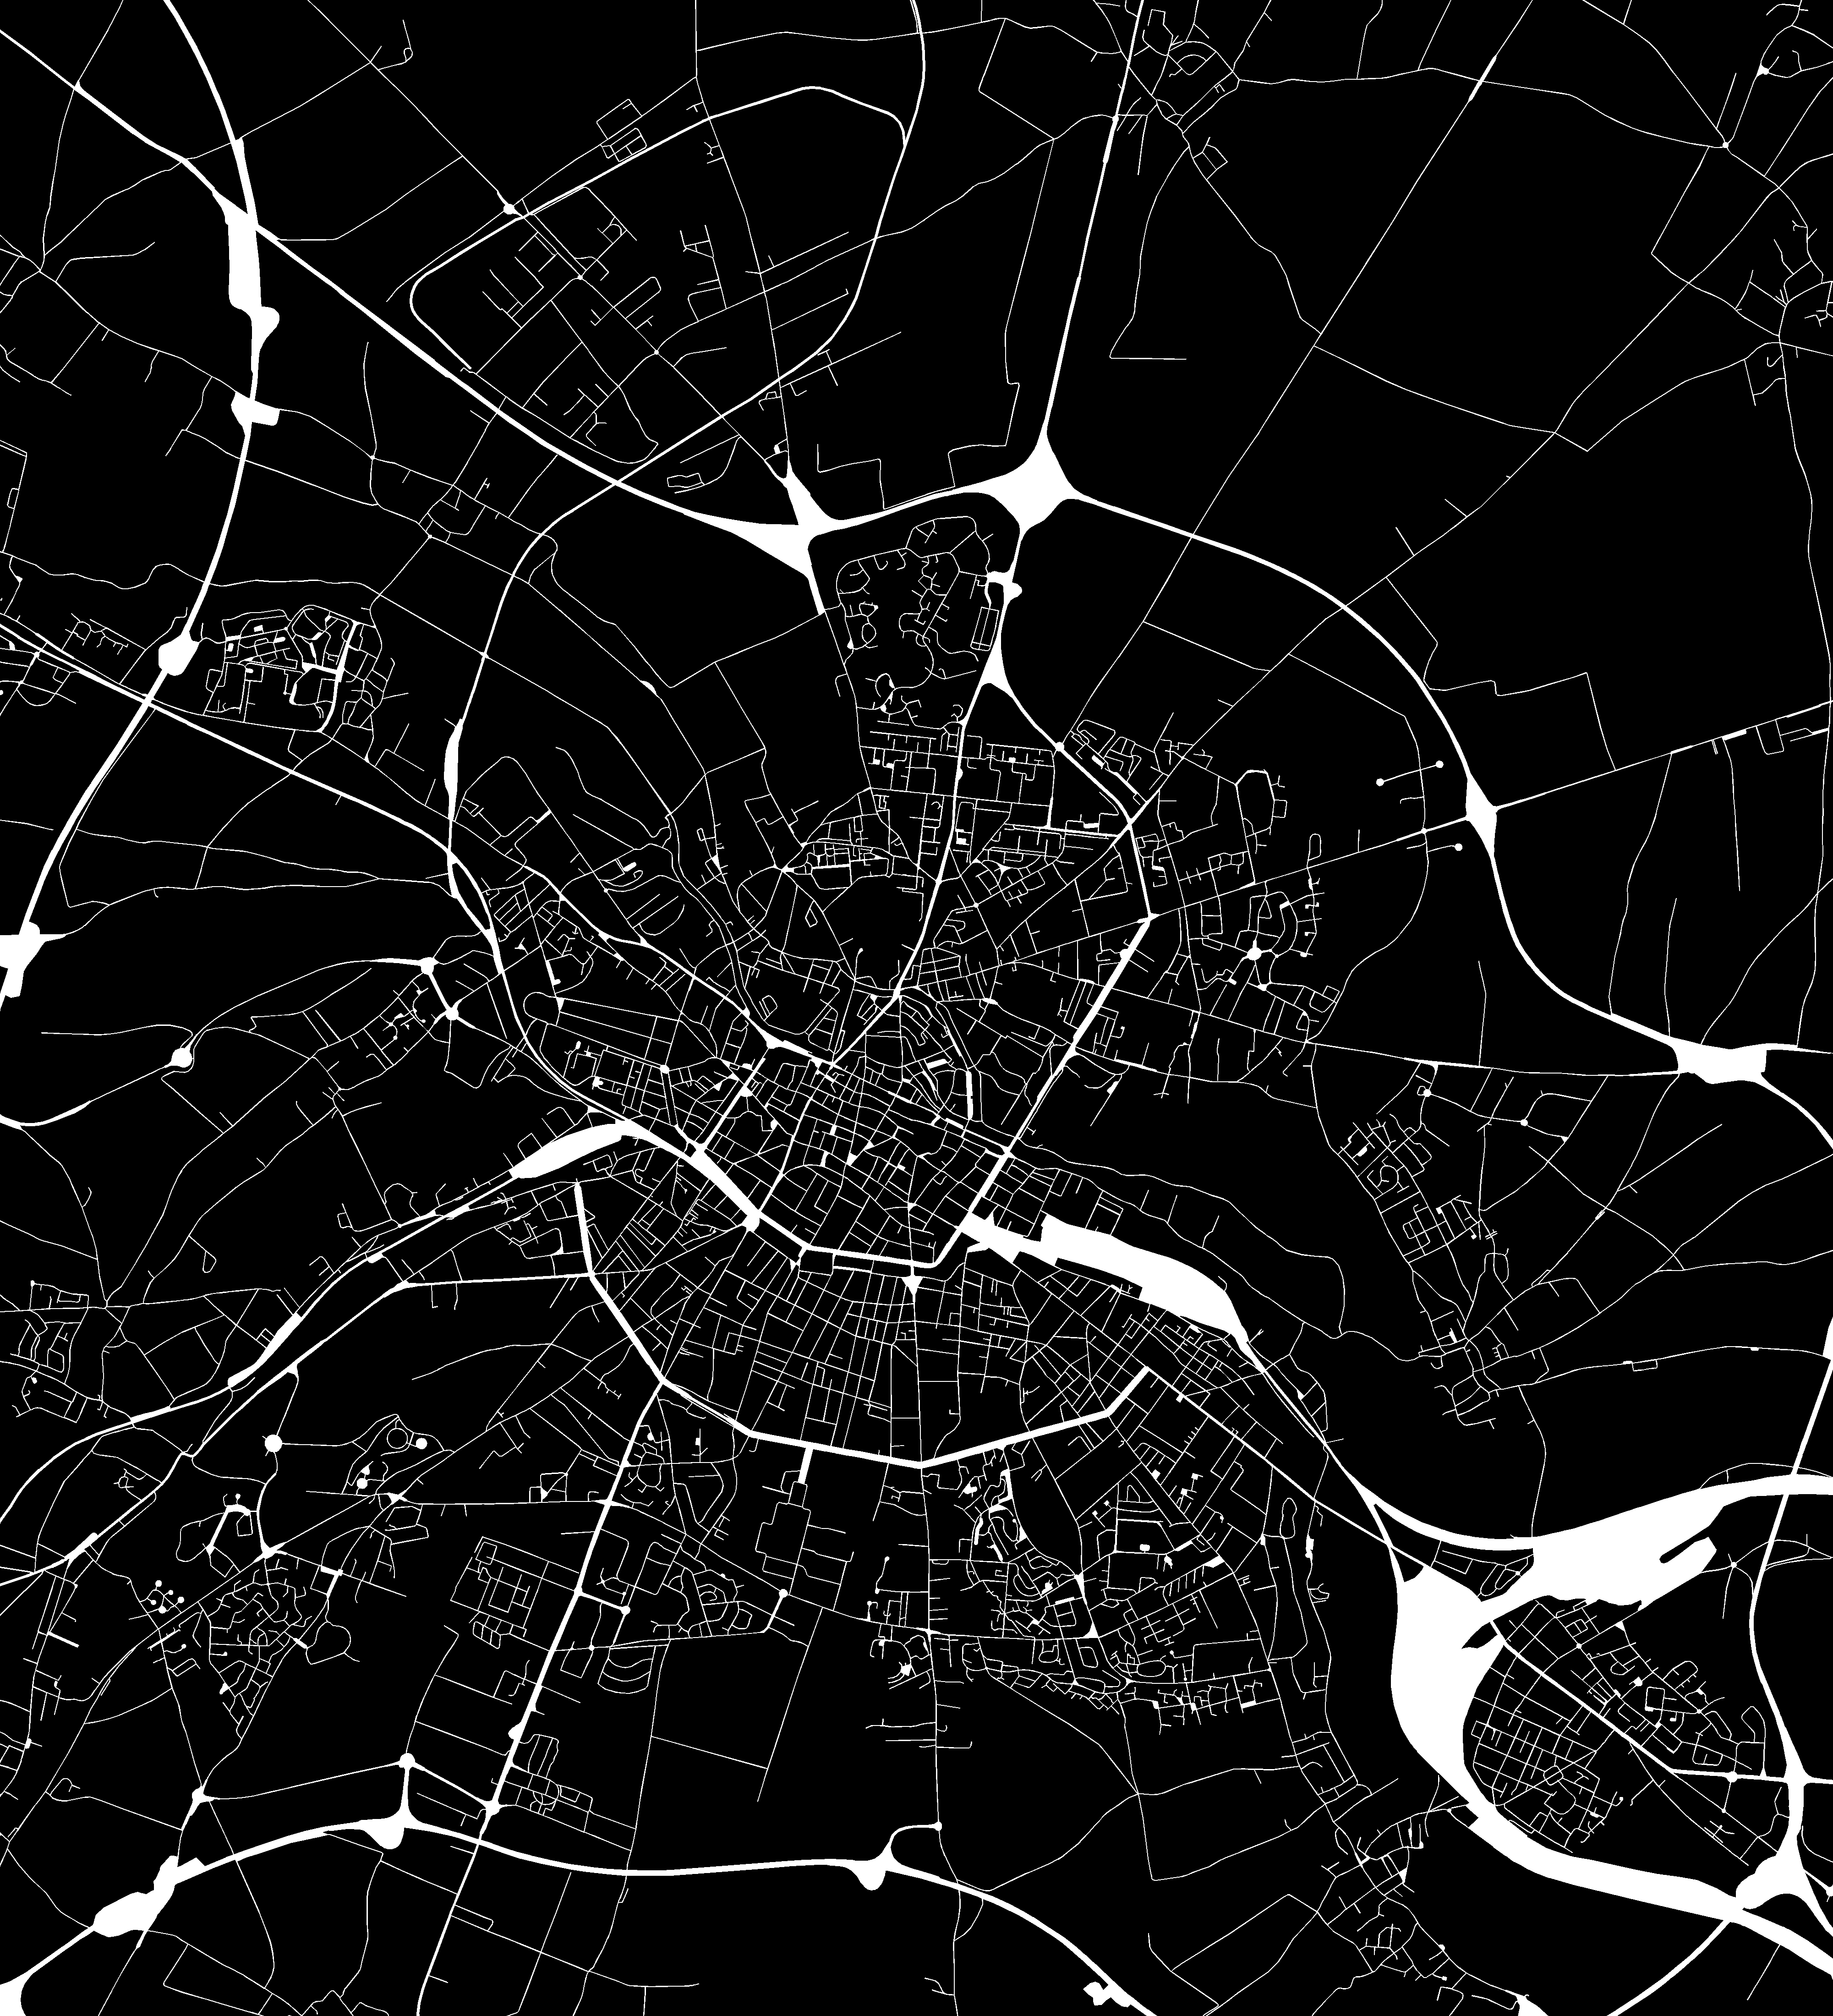
\includegraphics[width=0.7\textwidth]{amiens6_roads}
\caption{Immagine binaria della struttura cartografica di strade ed autostrade della regione di
Amiens: strade, autostrade e terreni ad esse collegati sono rappresentati con il bianco e lo sfondo in
nero.}

\label{fig:immagine_roads}

\end{figure}

In questo modo, si è riusciti a limitare la degradazione della classe
strade (classe 2) portandola ad un più che accettabile valore di
accuratezza ($64.61\%$); dal momento che il numero di pixel
classificati come strade non è molto significativo nella totalità dei
pixel dell'immagine, non si ha un'apprezzabile incremento dell'OA,
al
contrario della AA che, pesando gli errori uniformemente, registra un
significativo miglioramento ($63.54\%$).

In Figura \ref{fig:confrontoAmiens2012_2_5m} viene mostrato l'effetto
di questa \emph{feature} aggiuntiva per la classificazione delle
strade.

% (la porzione di immagine utilizzata è la stessa della Figura
%\ref{fig:confrontoAmiens2012_2_5m}, per una più immediata
%comprensione).

\begin{figure}[!ht]
\center
\subfigure[Mappa di classificazione senza HOG]{
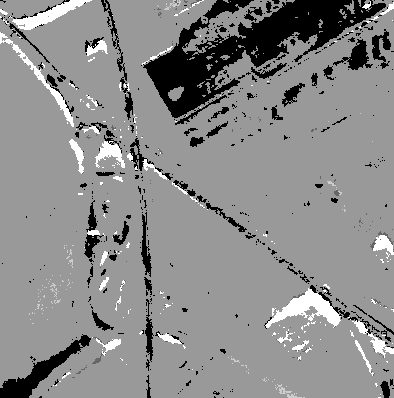
\includegraphics[width=0.35\textwidth]{ClassMap_Amiens2012_2_5m_riferimento}
}
\hspace{3mm}
\subfigure[Mappa di classificazione con HOG]{
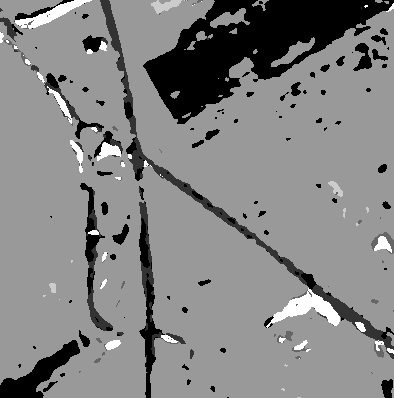
\includegraphics[width=0.35\textwidth]{ClassMap_Amiens2012_2_5m_HOG}
}
\\
\subfigure[Mappa di classificazione con HOG e cartografia]{
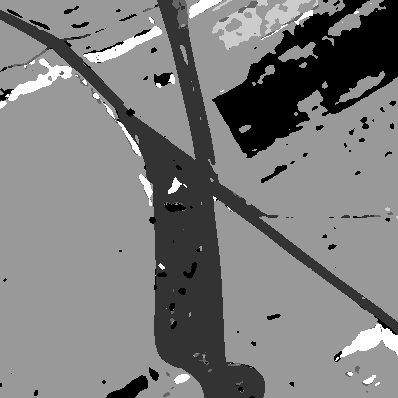
\includegraphics[width=0.35\textwidth]{ClassMap_Amiens2012_2_5m_HOG_and_roads}
}
\caption{Confronto su una porzione della periferia di Amiens di
$250\times250$ pixel della mappa di classificazione con e senza
estrazione di \emph{feature} HOG e con l'aggiunta della cartografia
stradale sul \emph{dataset} Amiens 2012 a $2.5$ m. }
\label{fig:confrontoAmiens2012_2_5m}
\end{figure}

\clearpage

\subsection{Amiens 2006 - 2.5m - 7 classi}

\'E riportata in Figura \ref{fig:ClassMap_Amiens2006_2_5m_roadsandhog}
la mappa di classificazione con \emph{feature} HOG aggiuntive in
configurazione di $4$ \emph{bins}, celle di dimensione $2\times2$
pixel e blocchi di normalizzazione con $16\times16$ pixel, con
filtraggio gaussiano sia per l'immagine in ingresso che per le
immagini HOG e con l'aggiunta della \emph{feature} cartografica delle
strade di Amiens.

\begin{figure}[!ht]

\center
\subfigure{
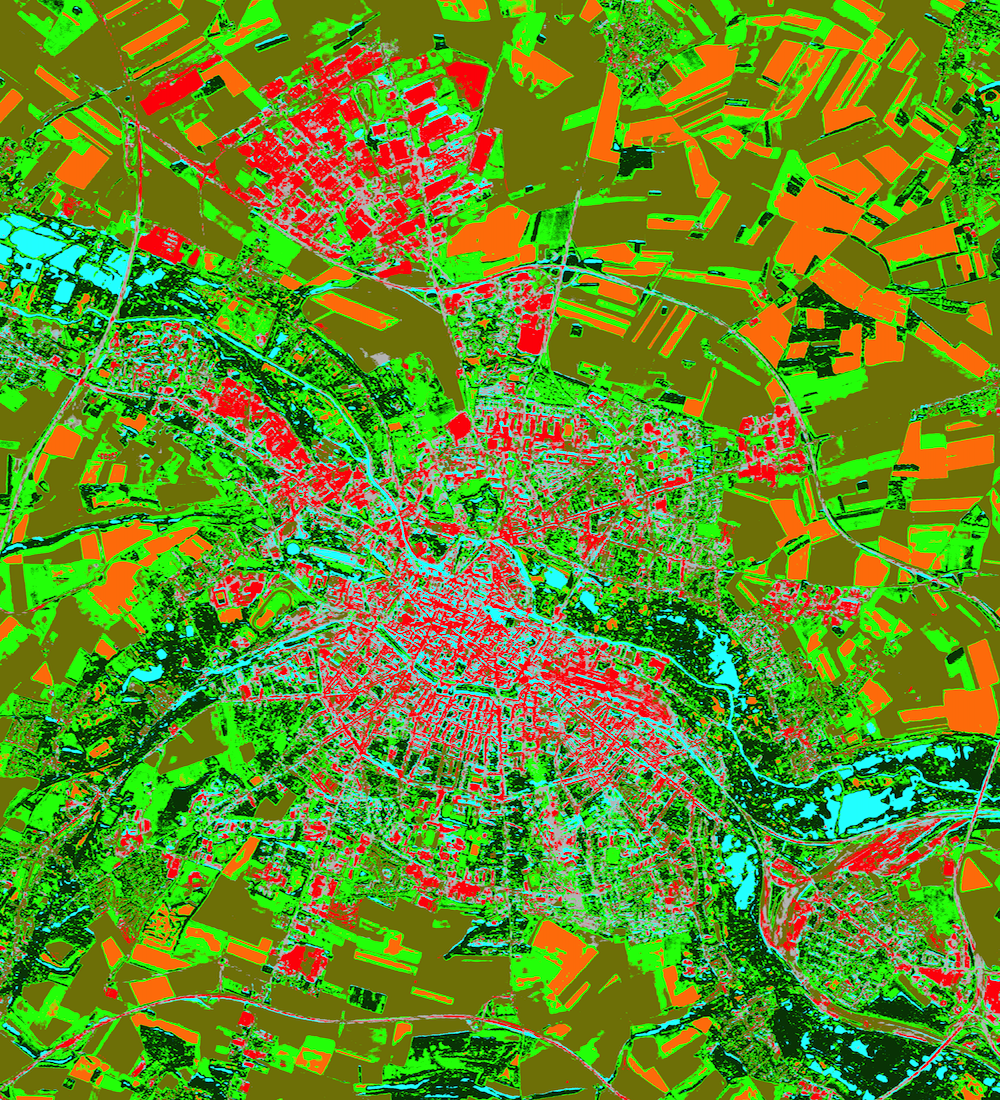
\includegraphics[width=0.7\textwidth]{ClassMap_Amiens2006_2_5m_roadsandhog}}
\\
\subfigure{
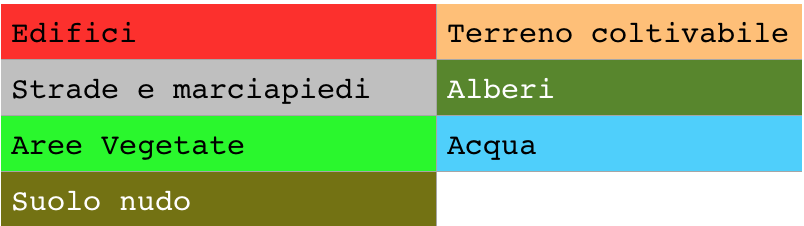
\includegraphics[width=0.35\textwidth]{Leggenda_7classi}}
\caption{Mappa di classificazione del dataset \emph{Amiens 2006 - 2.5m
- 7 classi}}
\label{fig:ClassMap_Amiens2006_2_5m_roadsandhog}

\end{figure}

Su questo \emph{dataset} i risultati sono stati interessanti, poichè
si differenziano notevolmente dai due casi studiati in precedenza.\\

E' innanzitutto importante far notare che questo esperimento ha
registrato il valore più alto a livello di OA ($74.88\%$) e AA
($70.61\%$). \\

L'analisi della matrice di confusione (riportata in Figura
\ref{fig:ClassMap_Amiens2006_2_5m_roadsandhog}) conferma il fatto che
il classificatore, per questo \emph{dataset}, si comporti mediamente
bene su tutte le classi, presentando accuratezze abbastanza elevate,
soprattutto in rapporto alla difficoltà del problema di
classificazione affrontato, per tutte le 7 classi presenti.\\L'unico
caso in cui i risultati non sono del tutto accettabili riguarda la
distinzione tra area vegetata (classe 3) e alberi (classe 6), i cui
pixel vengono spesso confusi tra le due categorie.

\begin{figure}[!ht]

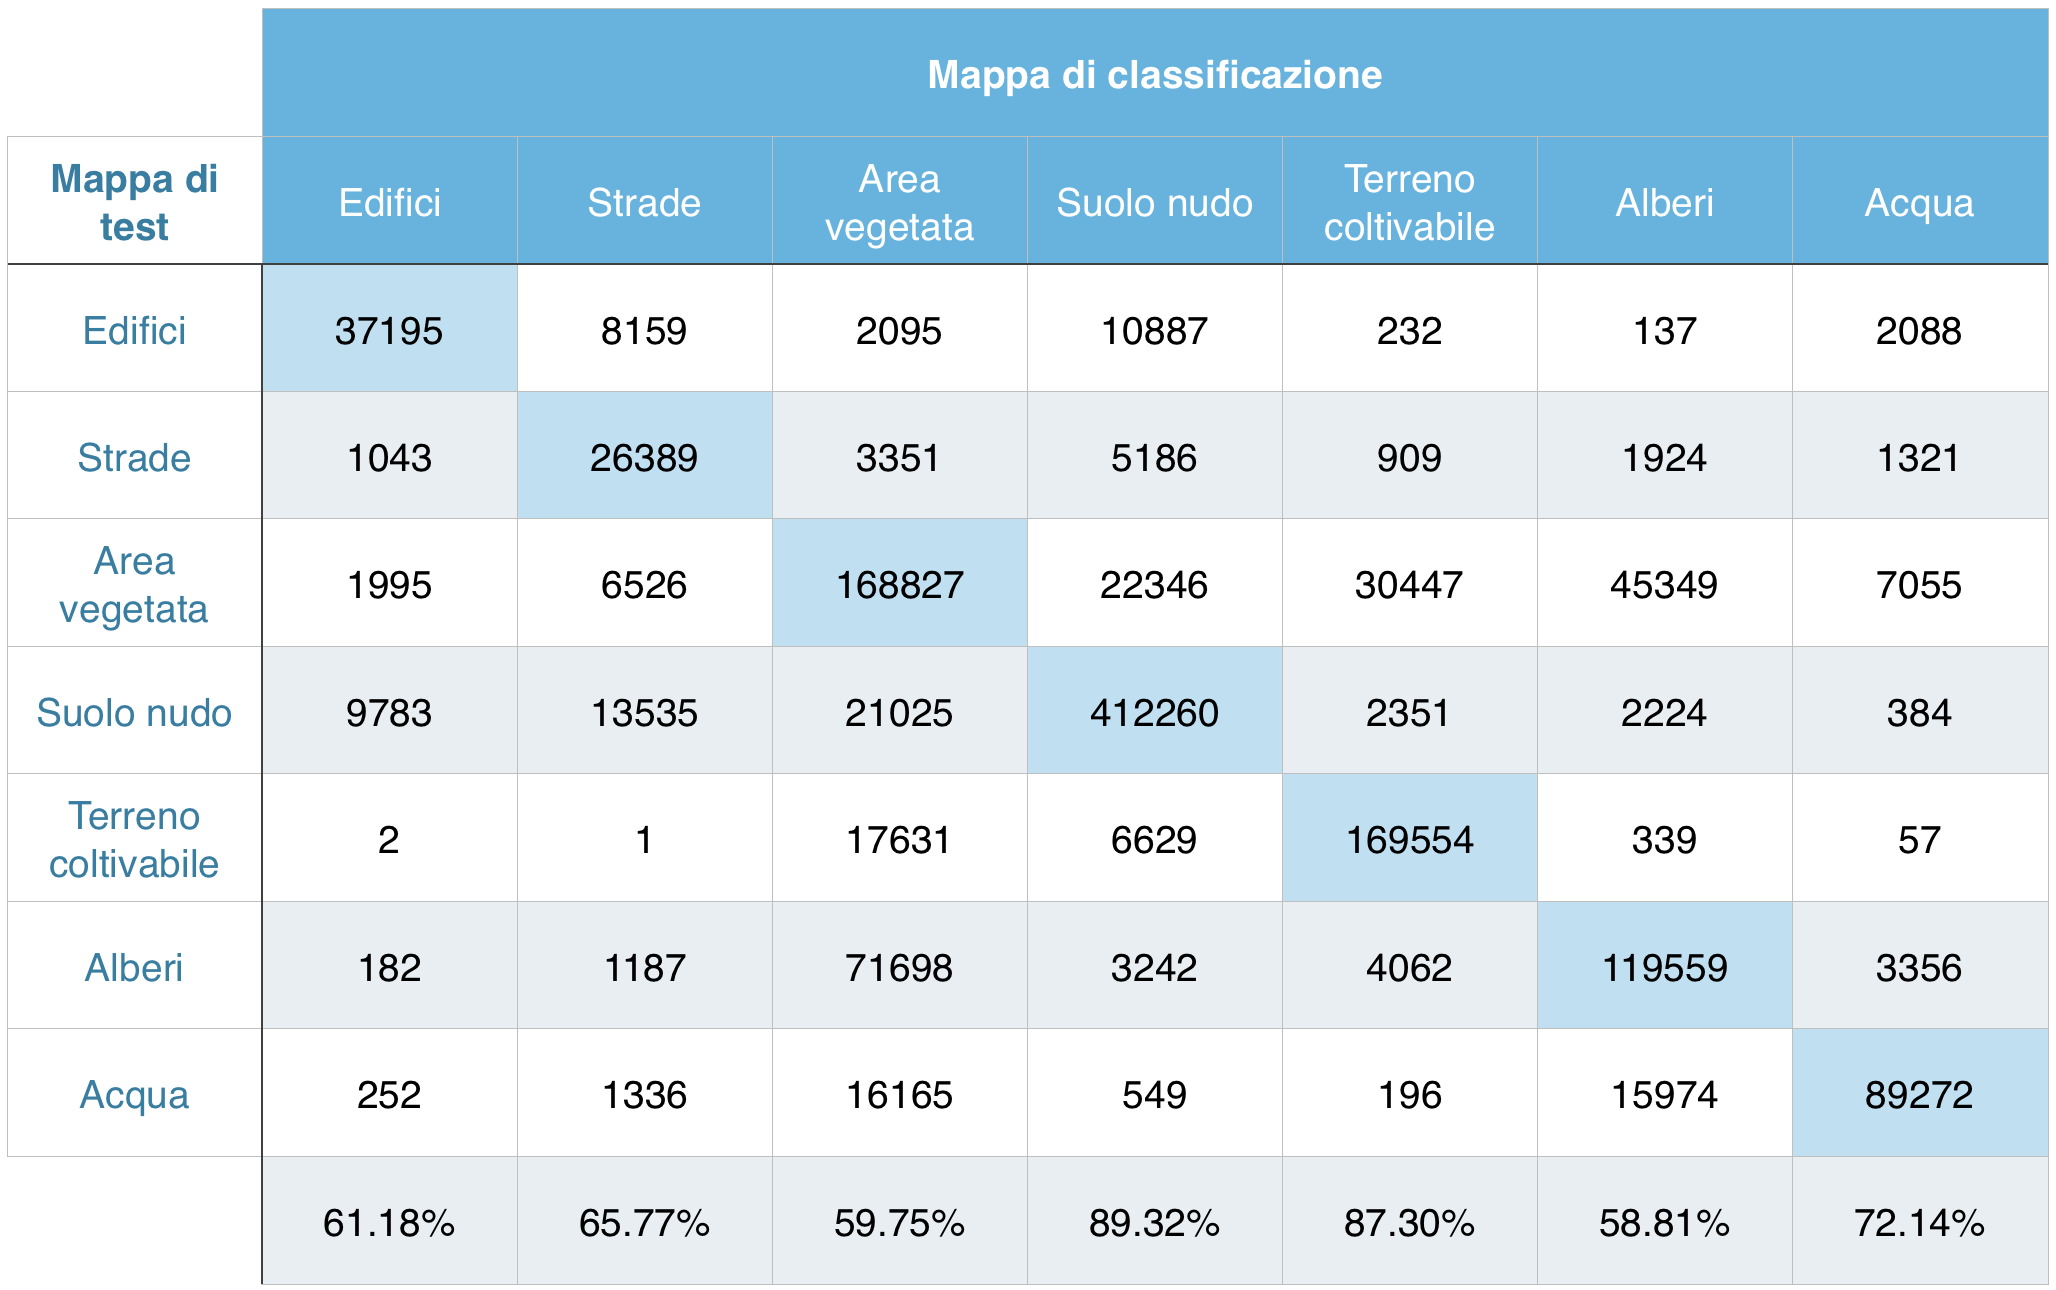
\includegraphics[width=1\textwidth]{Matrice_di_confusione_Amiens2006_2_5m_HOG_and_roads}

\caption{Mappa di classificazione del dataset \emph{Amiens 2006 - 2.5m
- 7 classi}}

\label{fig:Matrice_di_confusione_Amiens2006_2_5m_HOG_and_roads}

\end{figure}

In Figura \ref{fig:Confronto_Amiens2006_2_5m_con_e_senza_hog_e_roads}
vengono proposte le variazioni di prestazioni classe per classe nel
confronto fra questo risultato e quello ottenuto senza feature HOG.\\

\begin{figure}[!ht]

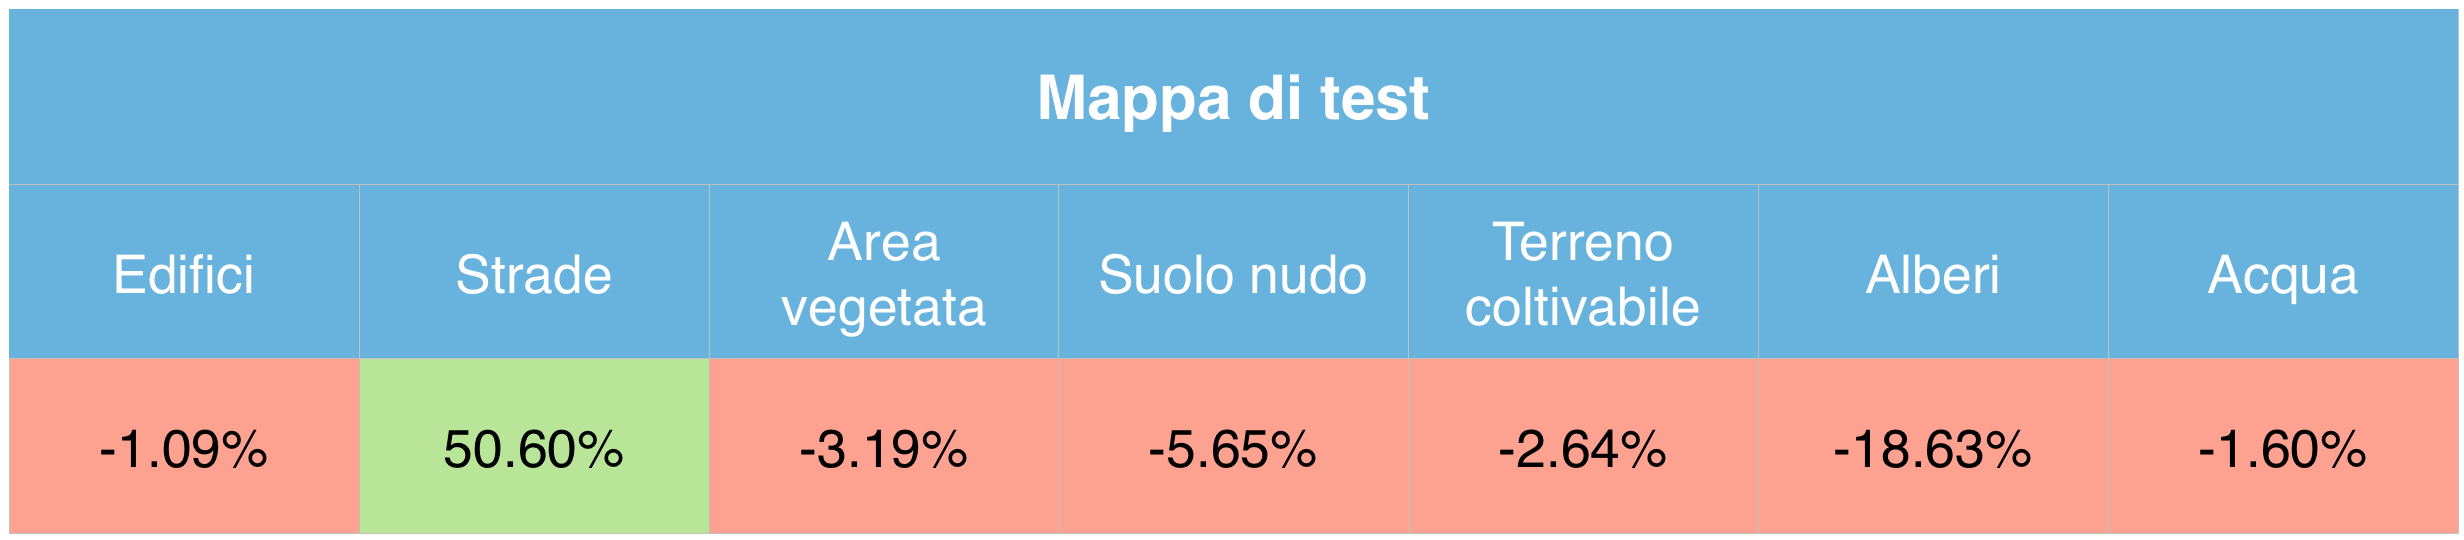
\includegraphics[width=1\textwidth]{Confronto_Amiens2006_2_5m_con_e_senza_hog_e_roads}

\caption{Differenze tra le accuratezze classe per classe con e
senza estrazione di \emph{feature} per il \emph{dataset} Amiens 2006 a
$2.5$ m}

\label{fig:Confronto_Amiens2006_2_5m_con_e_senza_hog_e_roads}

\end{figure}

Si osserva come l'introduzione delle \emph{feature} HOG peggiora quasi
tutti i valori di precisione del classificatore.\\

Tuttavia, come era possibile ipotizzare già dopo l'analisi dei due
precedenti esperimenti, l'uso di \emph{HOG}, unito all'aggiunta della
mappa cartografica, permette di far registrare un incremento notevole
alla classe deputata all'etichettatura delle strade, che senza HOG è
sempre la classe che registra i livelli di accuratezza più bassi,
spesso insufficienti a dare una buona rappresentazione della verità al
suolo. Tale risultato, insieme con quelli osservati in riferimento
agli altri due data set, suggerisce come l'uso di HOG in un problema
di classificazione a risoluzione spaziale abbastanza elevata in aree
urbane presenti benefici in termini di capacità di discriminazione di
classi con struttura geometrica ben definita, ma anche potenziali
svantaggi, soprattutto in riferimento all'identificazione di classi
prive di tale struttura a causa della loro natura fisica (ad es.,
alberi) o delle condizioni di acquisizione (ad es., sfocatura nei dati
o presenza di ombre).


%% VECCHIA VERSIONE
%In questo capitolo verranno presentati tre casi di studio e verrà fatta un'analisi delle prestazioni al variare dei parametri dell’algoritmo  HOG, evidenziando i valori ottimali individuti. 
%Successivamente verranno presentati i risultati ottenuti valutando anche gli aspetti per cui questo algoritmo ha dato risultati parzialmente soddisfacenti.
%
%\clearpage
%
%\section{Descrizione dei \emph{dataset}}
%In questa tesi sono stati analizzati tre casi rilevanti, tutti relativi alla classificazione dell'area urbana di Amiens (Francia).  Si tratta di un problema di classificazione interessante e particolarmente complesso, in quanto le regioni coinvolte sono caratterizzate sia da aree omogenee (come corsi d'acqua) sia da strutture geometriche ben definite (come edifici e strade) e zone di suolo con\emph{ pattern} regolari (come campi coltivabili e non).\\
%L'analisi condotta ha coinvolto l'uso di immagini ad elevata risoluzione spaziale, acquisite nell'ambito di un progetto europeo dedicato allo sviluppo di tecnologie ICT innovative per l'identificazione di aree urbane attualmente non usate e potenzialmente riqualificabili.\\
%
%Il \emph{dataset} per ogni esperimento è costituito da un'immagine telerilevata, dalla mappa di \emph{training} e dalla mappa di \emph{testing} corrispondenti.
%Le immagini telerilevate sono state acquisite dal sensore passivo \textsc{SPOT5 HRG} a tre canali, corrispondenti alle lunghezze d'onda del verde (G, $495 - 570\text{ } nm$), del rosso (R, $620 -  750\text{ } nm$) e del vicino infrarosso (NIR, \emph{Near InfraRed} $0.75 - 1.4\text{ } \mu m$).
%Sebbene i canali spettrali di SPOT5 HRG avrebbero risoluzione spaziale nativa di 10 m, il sensore stesso acquisisce anche un canale pancromatico, associato all'intero intervallo di lunghezza d'onda (dal visibile al vicino infrarosso) e caratterizzato da risoluzione spaziale di 5 m. In fase di pre-elaborazione, tecniche di \emph{pansharpening}\footnote{Pansharpening è un processo di fusione di immagini pancromatiche ad alta risoluzione con immagini multispettrale a risoluzione inferiore per creare una singola immagine multispettrale ad alta risoluzione.} sono state applicate al fine di fondere le informazione fornite dai dati multispettrali e pancromatici e generare un'immagine G-R-NIR a risoluzione spaziale di 5 m. Inoltre, SPOT5 HRG permette anche acquisizioni di coppie stereo di immagini. L'applicazione di tecniche di super-risoluzione ad una di tali coppie permette di generare un'ulteriore immagine volta a stimare la distribuzione spaziale della radianza ricevuta ad una risoluzione di 2.5 m. Sono stati usati a fini di sperimentazione dati ottenuti da entrambe le tipologie di pre-elaborazione e quindi caratterizzati da pixel di dimensione pari a 2.5 e 5 m.
% 
%
%\subsection{Amiens 2006 - 5m - 10 classi}
%L'immagine \emph{Amiens6--5m} è stata acquisita nel 2006 e ha pixel di dimensione spaziale pari a $5 \text{m}$, coprendo approssimativamente un'area di $10\text{ }km\times11\text{ }km$ ($2000\times2200$ pixel).\\
%L'insieme delle classi $\Omega=\left\lbrace\omega_1,\omega_2,\ldots,\omega_{10}\right\rbrace$ che costituisce questo primo esperimento è il seguente:
%\begin{enumerate}
%\item Area urbana ad alta densità
%\item Area urbana a bassa densità
%\item Strade
%\item Area verde urbana 
%\item Suolo nudo
%\item Terreno coltivabile
%\item Terreno non coltivabile 
%\item Alberi
%\item Corsi d'acqua
%\item Specchi d'acqua
%\end{enumerate}
%Nella Figura \ref{fig: Amiens65m} vengono presentate le immagini caratterizzanti il primo \emph{dataset}. 
%\begin{lstlisting}[float=b,title={Distribuzione dei pixel di training (TR) e test (TS) classe per classe.},
%                   label=lst:esempio, frame=lines]
%TR:				TE:
%Class 1 : 72483 		Class 1 : 70299
%Class 2 : 149917 	Class 2 : 68435
%Class 3 : 17945 		Class 3 : 10019
%Class 4 : 25121 		Class 4 : 16012
%Class 5 : 233481 	Class 5 : 115570
%Class 6 : 113030 	Class 6 : 48615
%Class 7 : 62854 		Class 7 : 54582
%Class 8 : 90718 		Class 8 : 50701
%Class 9 : 7903 		Class 9 : 3012
%Class 10: 34833 		Class 10: 27924
%Total   : 808285		Total   : 465169
%\end{lstlisting}
%\clearpage
%\begin{figure}[!ht]
%   \center
%   \subfigure[Immagine telerilevata]{
%      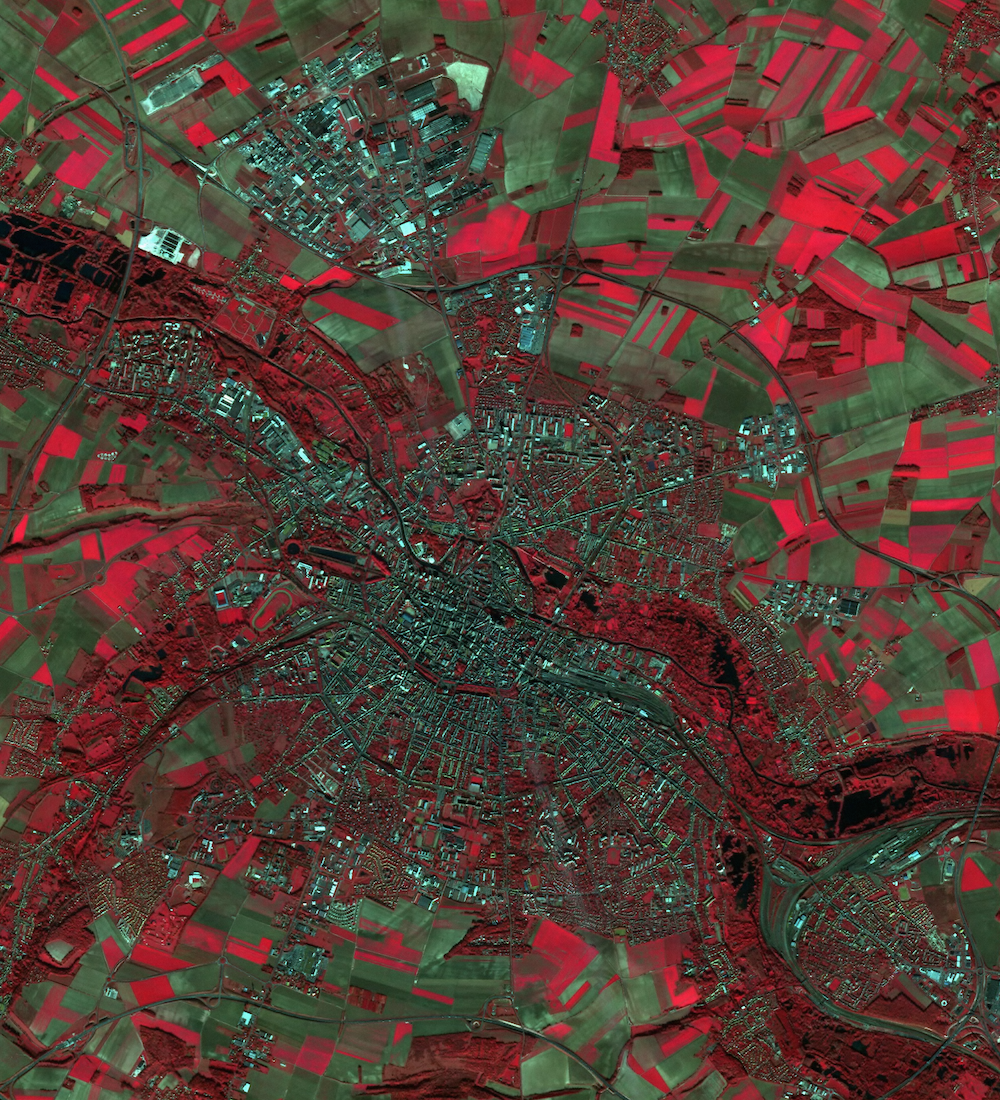
\includegraphics[width=0.7\textwidth]{Amiens_2006_SPOT_5m}}\\%pdf0.45
%         \subfigure[Mappa di \emph{training}]{
%      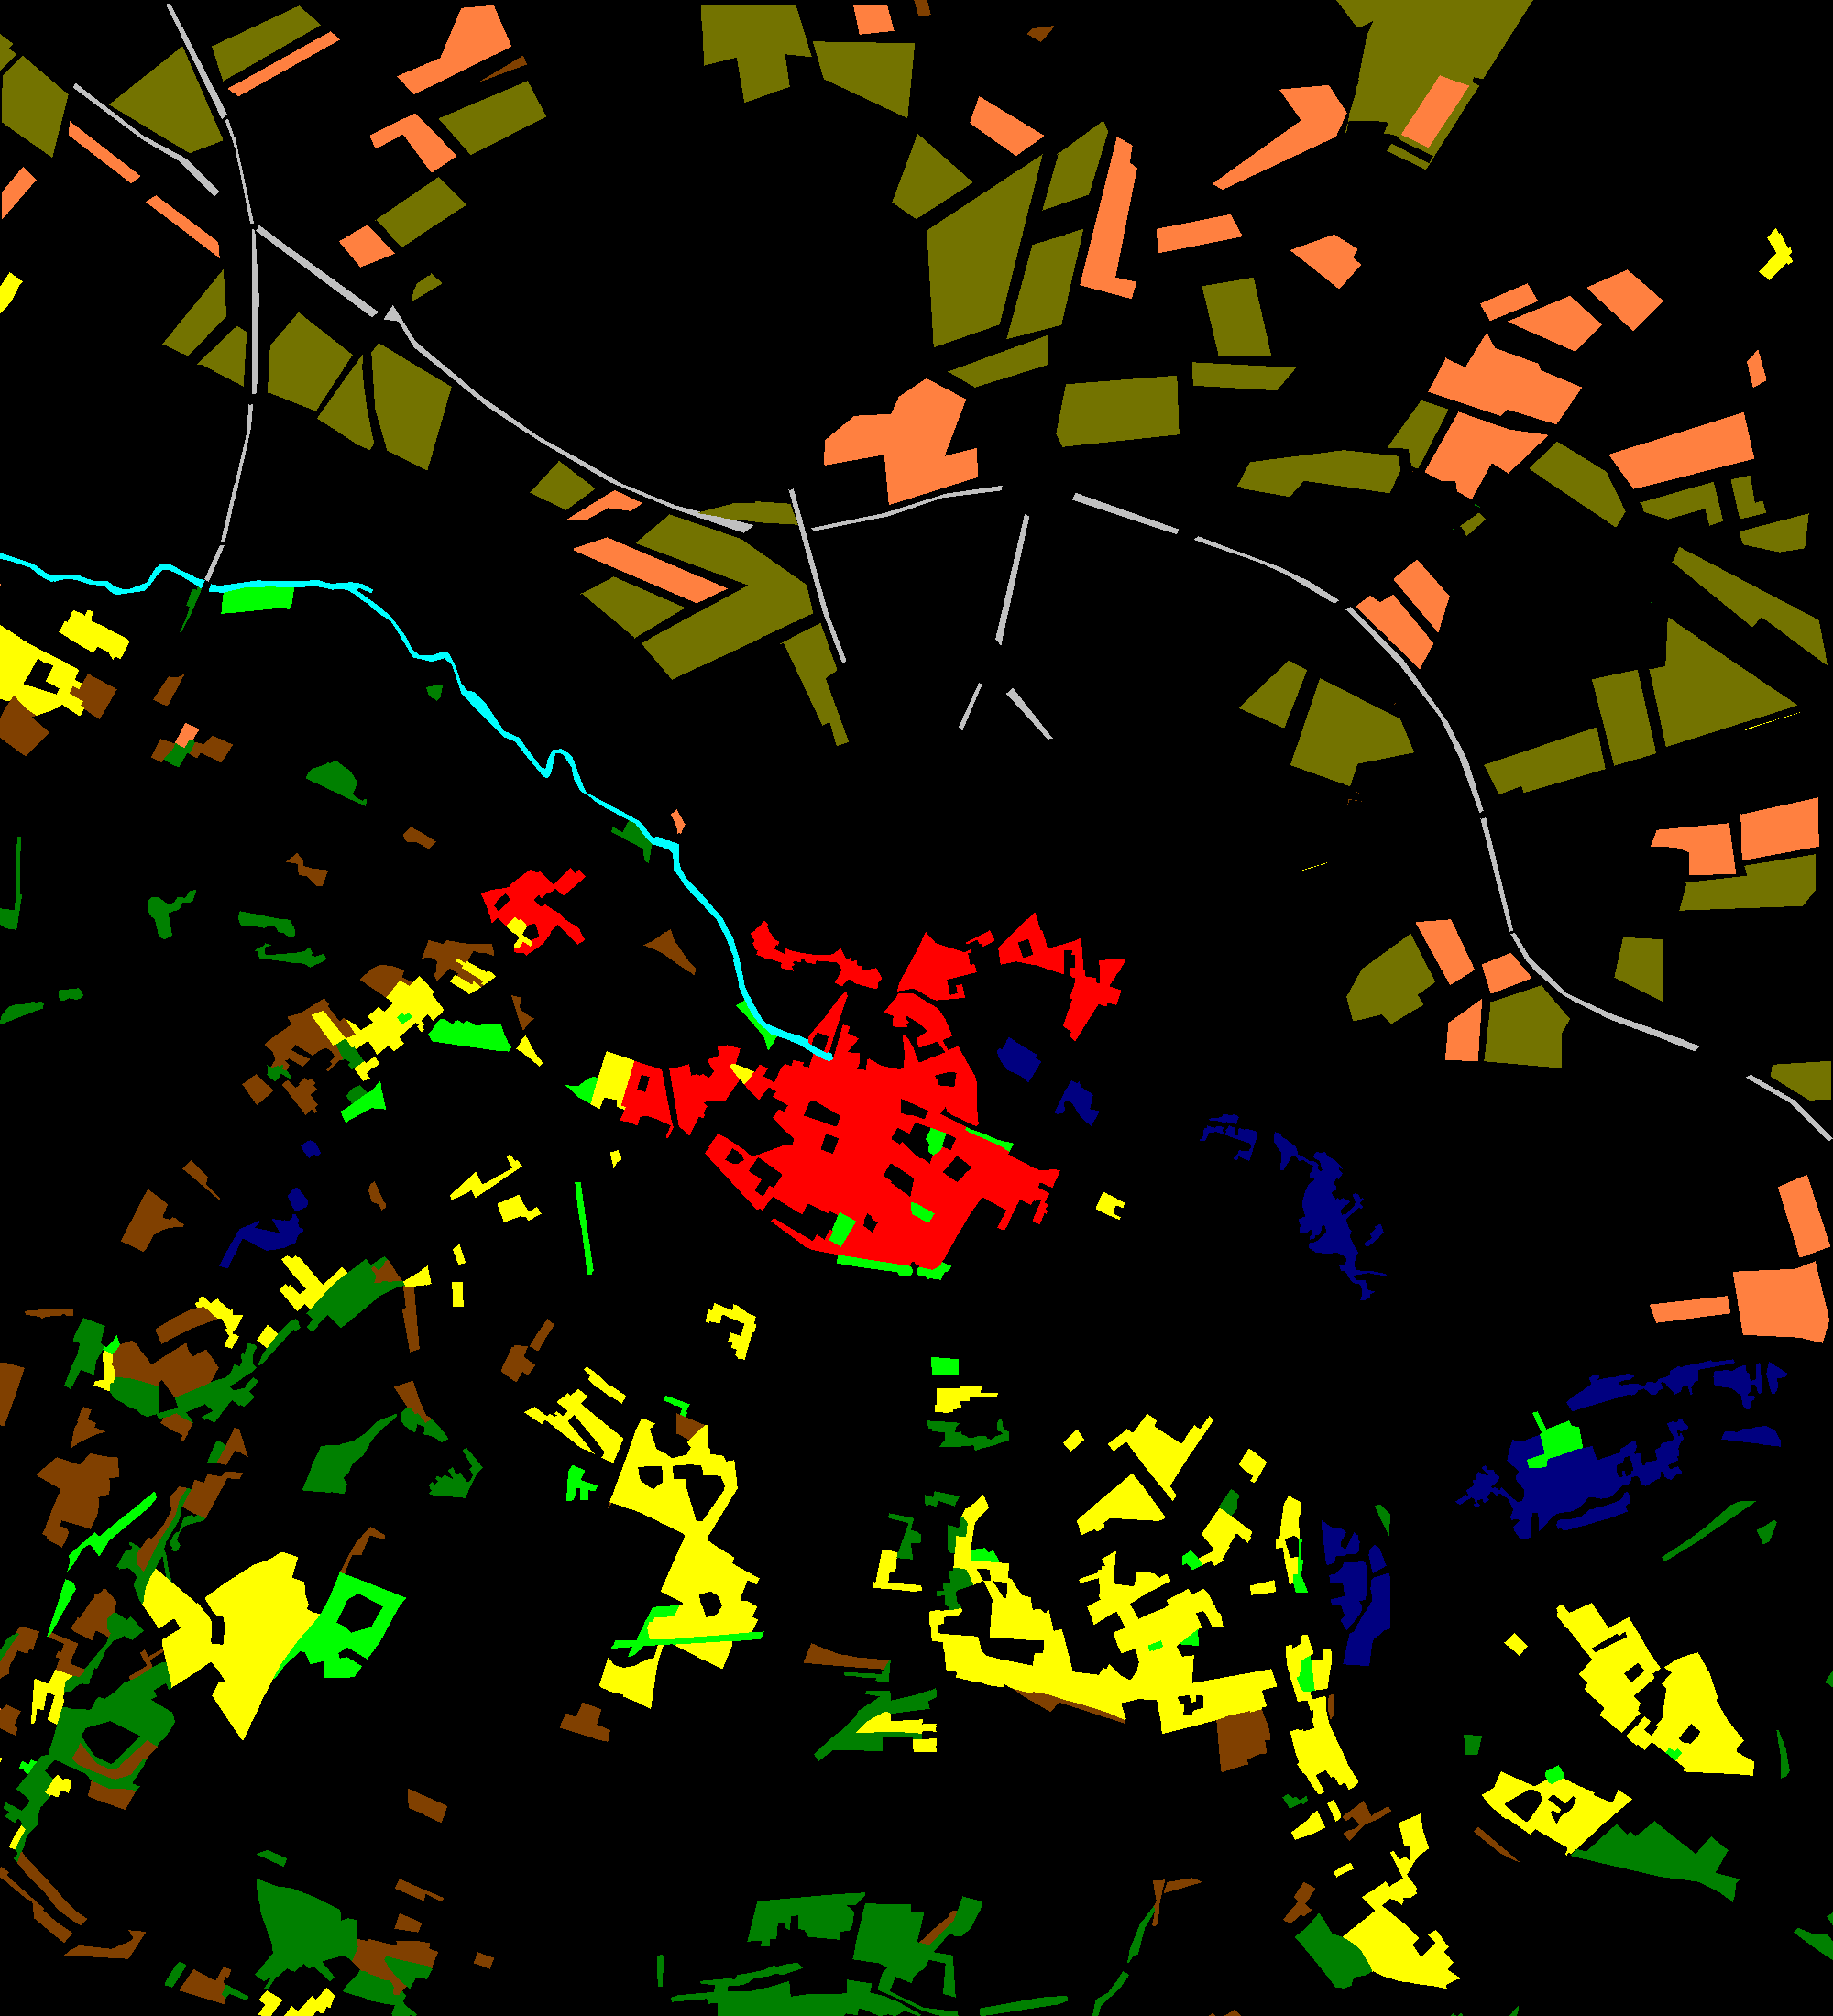
\includegraphics[width=0.4\textwidth]{GT_Amiens2006_5m_10classes_TR}}
%     \hspace{4mm}
%    \subfigure[Legenda classi della mappa di \emph{training}]{
%      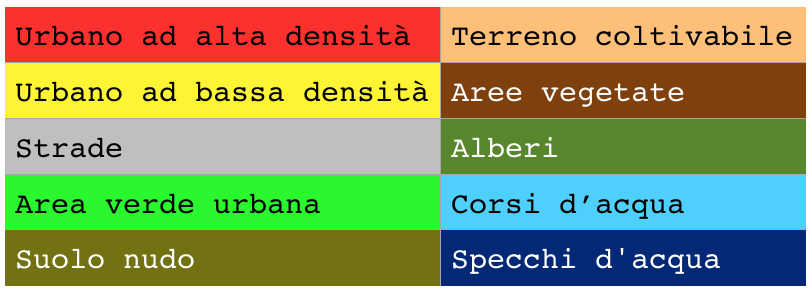
\includegraphics[scale=0.5]{Leggenda_2006_10classi}}
%    \caption{\emph{Dataset} con immagine RBG in falso colore ($2000\times2200$ pixel) acquisita su Amiens (Francia) dal sensore \textsc{SPOT5 HRG}}
%    \label{fig: Amiens65m}
%  \end{figure}
%  
%\clearpage
%\subsection{Amiens 2006 - 2.5m - 7 classi}
%L'immagine \emph{Amiens6--2.5m} è stata acquisita sempre nel 2006, ma ha pixel di dimesione spaziale pari a $2.5\text{ }m$  e copre sempre approssimativamente un'area di $10\text{ }km\times11\text{ }km$ ($4001\times4400$ pixel).\\
%L'insieme delle classi $\Omega=\left\lbrace\omega_1,\omega_2,\ldots,\omega_{7}\right\rbrace$ che costituisce il secondo \emph{dataset} è il seguente:
%\begin{enumerate}
%\item Edifici
%\item Strade e marciapiedi
%\item Aree vegetate
%\item Suolo nudo
%\item Terreno coltivabile
%\item Alberi
%\item Acqua
%\end{enumerate}
%Nella Figura \ref{fig: Amiens62_5m} vengono presentate le immagini caratterizzanti il secondo \emph{dataset}. Nella Figura \ref{fig:3classi} sono riportate, per una migliore comprensione, la distribuzione dei pixel di\emph{ training} di tre classi diverse (nero = strade, blu = acqua, verde = aree vegetate), rispetto a due distinte coppie di \emph{feature} spettrali. Tali grafici evidenziano come alcune classi siano spettralmente molto sovrapposte e confermano l'opportunità dell'estrazione di feature aggiuntive associate alla distribuzione spaziale delle intensità dei pixel invece che all'informazione spettrale da essi apportata. Inoltre è importante notare come l'immagine a 2.5 m sia visibiamente più sfocata di quella a 5 m. Ciò è legato all'efficacia solo parziale del metodo di super-risoluzione che, in fase di pre-elaborazione, fu applicato. Pertanto, la risoluzione spaziale di tale immagine, ossia la dimensione del più piccolo dettaglio distinguibile, si ritiene peggiore di 2.5 m. Ciò rende il processo di classificazione ulteriormente complesso.
%
% \begin{figure}[!ht]
%\center  
%\subfigure{
%      \includegraphics[width=0.35\textwidth]{AssiRG_3classi}}
%      \hspace{3mm}
%\subfigure{ 
%		 \includegraphics[width=0.35\textwidth]{AssiGB_3classi}}
%		
%    \caption{Analisi della distribuzione di tre classi rispetto a due coppie di \emph{feature} spettrali}
%    \label{fig:3classi}
%  \end{figure}
%
%
%\clearpage
%
%\begin{figure}[!ht]
%   \center
%   \subfigure[Immagine telerilevata]{
%      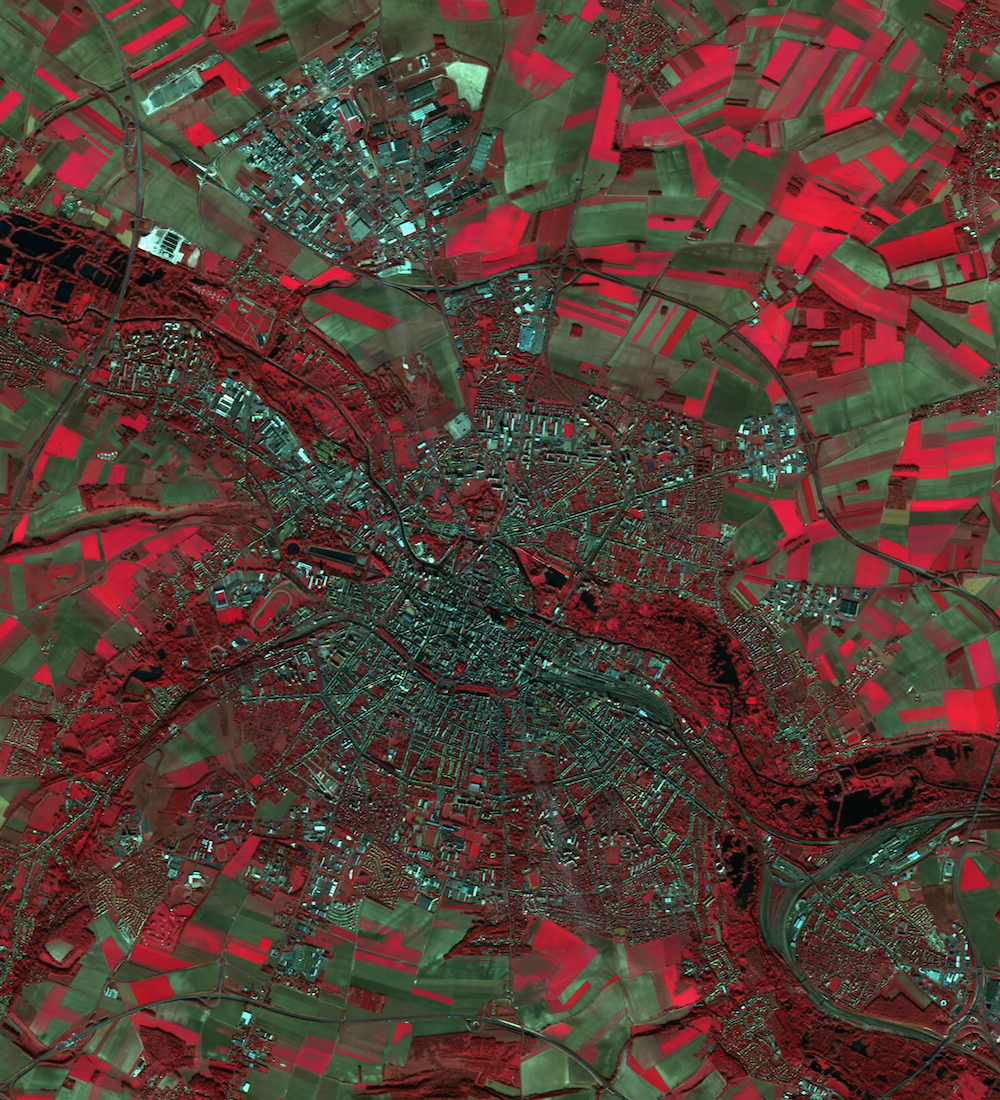
\includegraphics[width=0.7\textwidth]{Amiens_2006_SPOT_2_5m}}\\%pdf0.45
%         \subfigure[Mappa di \emph{training}]{
%      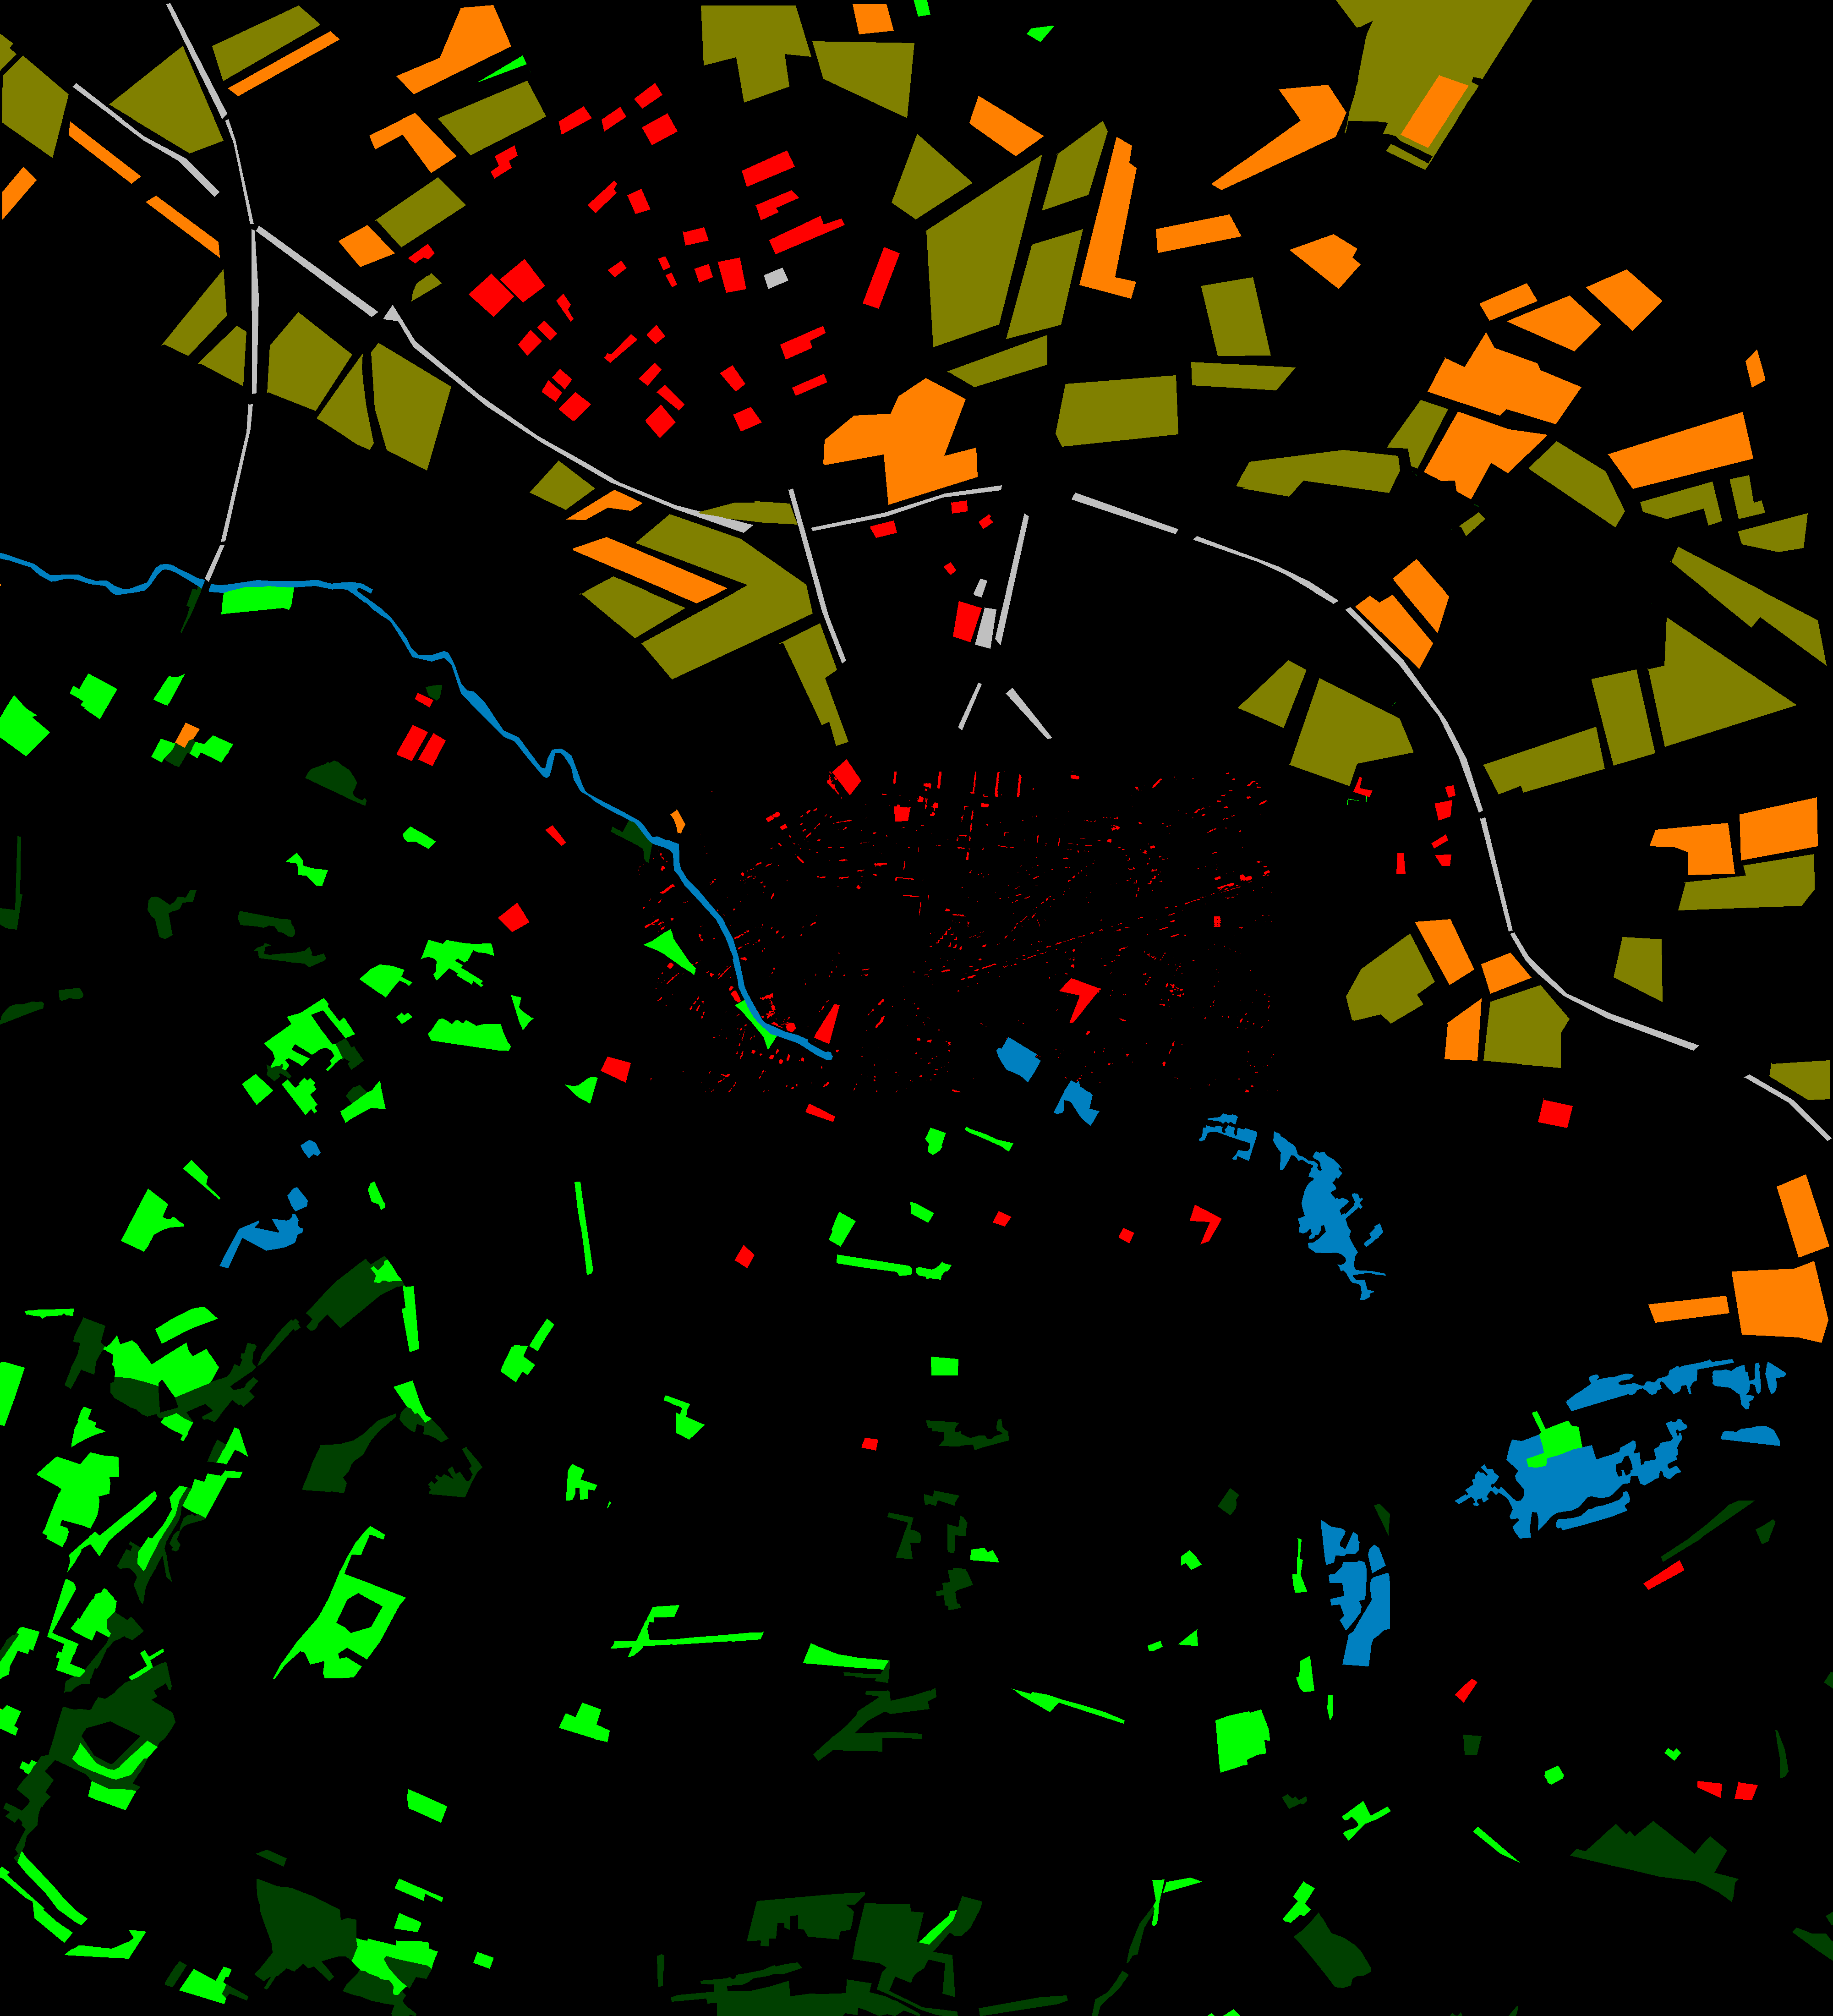
\includegraphics[width=0.4\textwidth]{GT_Amiens2006_2_5m_7classes_TR}}
%     \hspace{4mm}
%    \subfigure[Legenda classi della mappa di \emph{training}]{
%      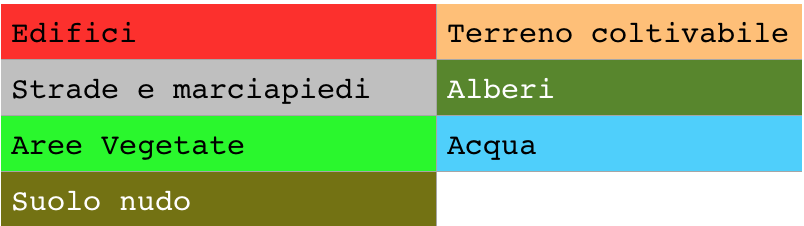
\includegraphics[scale=0.5]{Leggenda_7classi}}
%    \caption{\emph{Dataset} con immagine RBG in falso colore ($4001\times4400$ pixel) acquisita su Amiens (Francia) dal sensore \textsc{SPOT5 HRG} nel 2006}
%    \label{fig: Amiens62_5m}
%  \end{figure}
%\clearpage
%
%
%\subsection{Amiens 2012 - 2.5m - 7 classi}
%L'immagine \emph{Amiens12--2.5m} è stata acquisita nel 2012 e ha pixel di dimensione spaziale pari a $2.5\text{ }m$, coprendo sempre un'area di circa $10\text{ }km\times11\text{ }km$ ($4001\times4400$ pixel).\\
%L'insieme delle classi $\Omega=\left\lbrace\omega_1,\omega_2,\ldots,\omega_{7}\right\rbrace$, che costituisce il \emph{dataset}, è lo stesso del precedente. Per uniformità vengono ugualmente riportate:
%\begin{enumerate}
%\item Edifici
%\item Strade e marciapiedi
%\item Aree vegetate
%\item Suolo nudo
%\item Terreno coltivabile
%\item Alberi
%\item Acqua
%\end{enumerate}
%Nella Figura \ref{fig: Amiens122_5m} vengono presentate le immagini caratterizzanti il primo \emph{dataset}; si osservi con attenzione la composizione dell'immagine di \emph{training}.\\
%Anche in questo caso si nota come l'immagine a 2.5 m sia sfocata, rendendo il processo di classificazione largamente complesso. Infatti, la risoluzione spaziale di tale immagine è da ritenersi peggiore di 2.5 m, sempre a causa della parziale efficazia del metodo di super-risoluzione applicato in fase di pre-elaborazione.
%
%\begin{lstlisting}[float=b,title={Distribuzione dei pixel di training(TR) e test(TS) classe per classe.},
%                   label=lst:esempio, frame=lines]
%TR:					TE:
%Class 1: 132005				Class 1: 60793
%Class 2: 76330				Class 2: 40123
%Class 3: 351949				Class 3: 282545
%Class 4: 933512				Class 4: 461562
%Class 5: 451999				Class 5: 194213
%Class 6: 363058				Class 6: 203286
%Class 7: 170921				Class 7: 123744
%Total  : 2479774			Total  : 1366266
%\end{lstlisting}
%\clearpage
%
%\begin{figure}[!ht]
%   \center
%   \subfigure[Immagine telerilevata]{
%      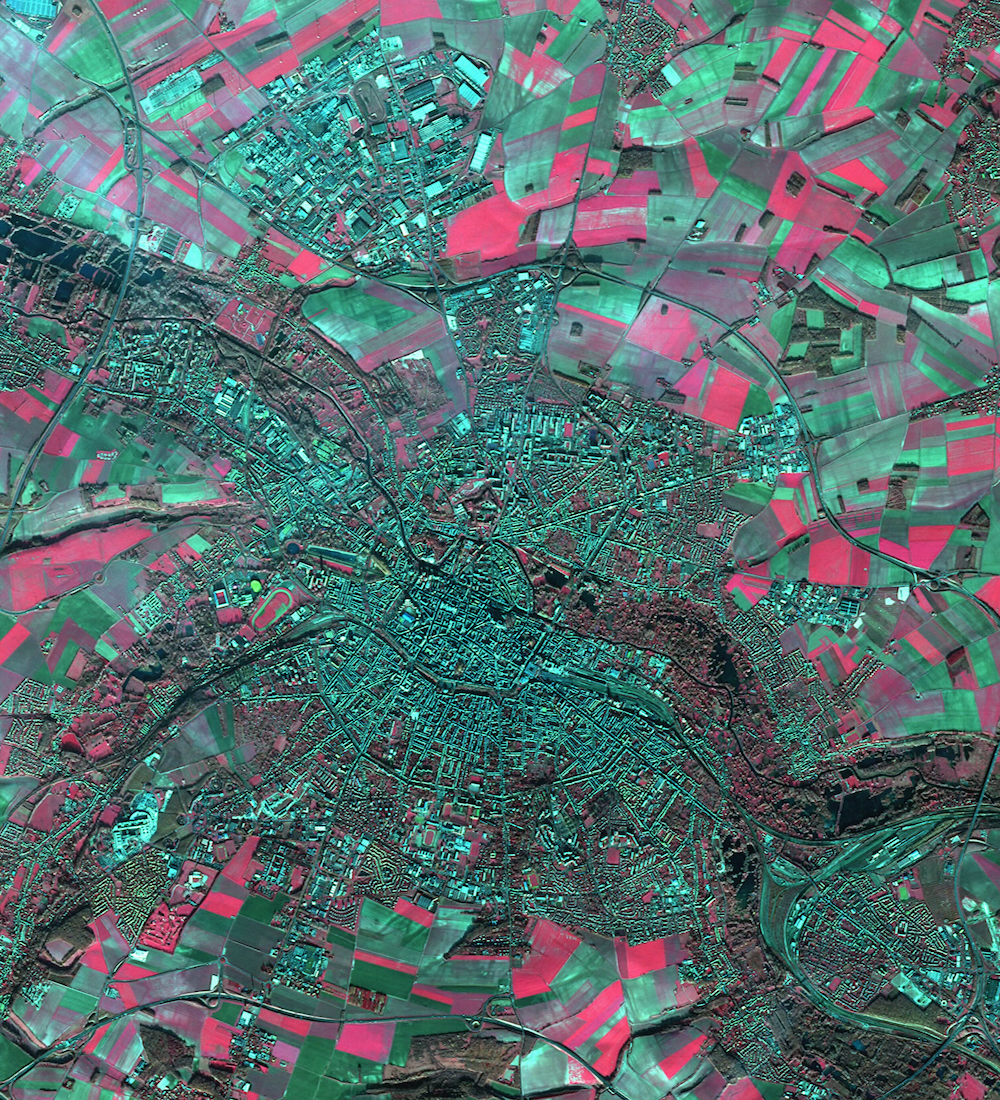
\includegraphics[width=0.7\textwidth]{Amiens_2012_SPOT_2_5m}}\\%pdf0.45
%         \subfigure[Mappa di \emph{training}]{
%      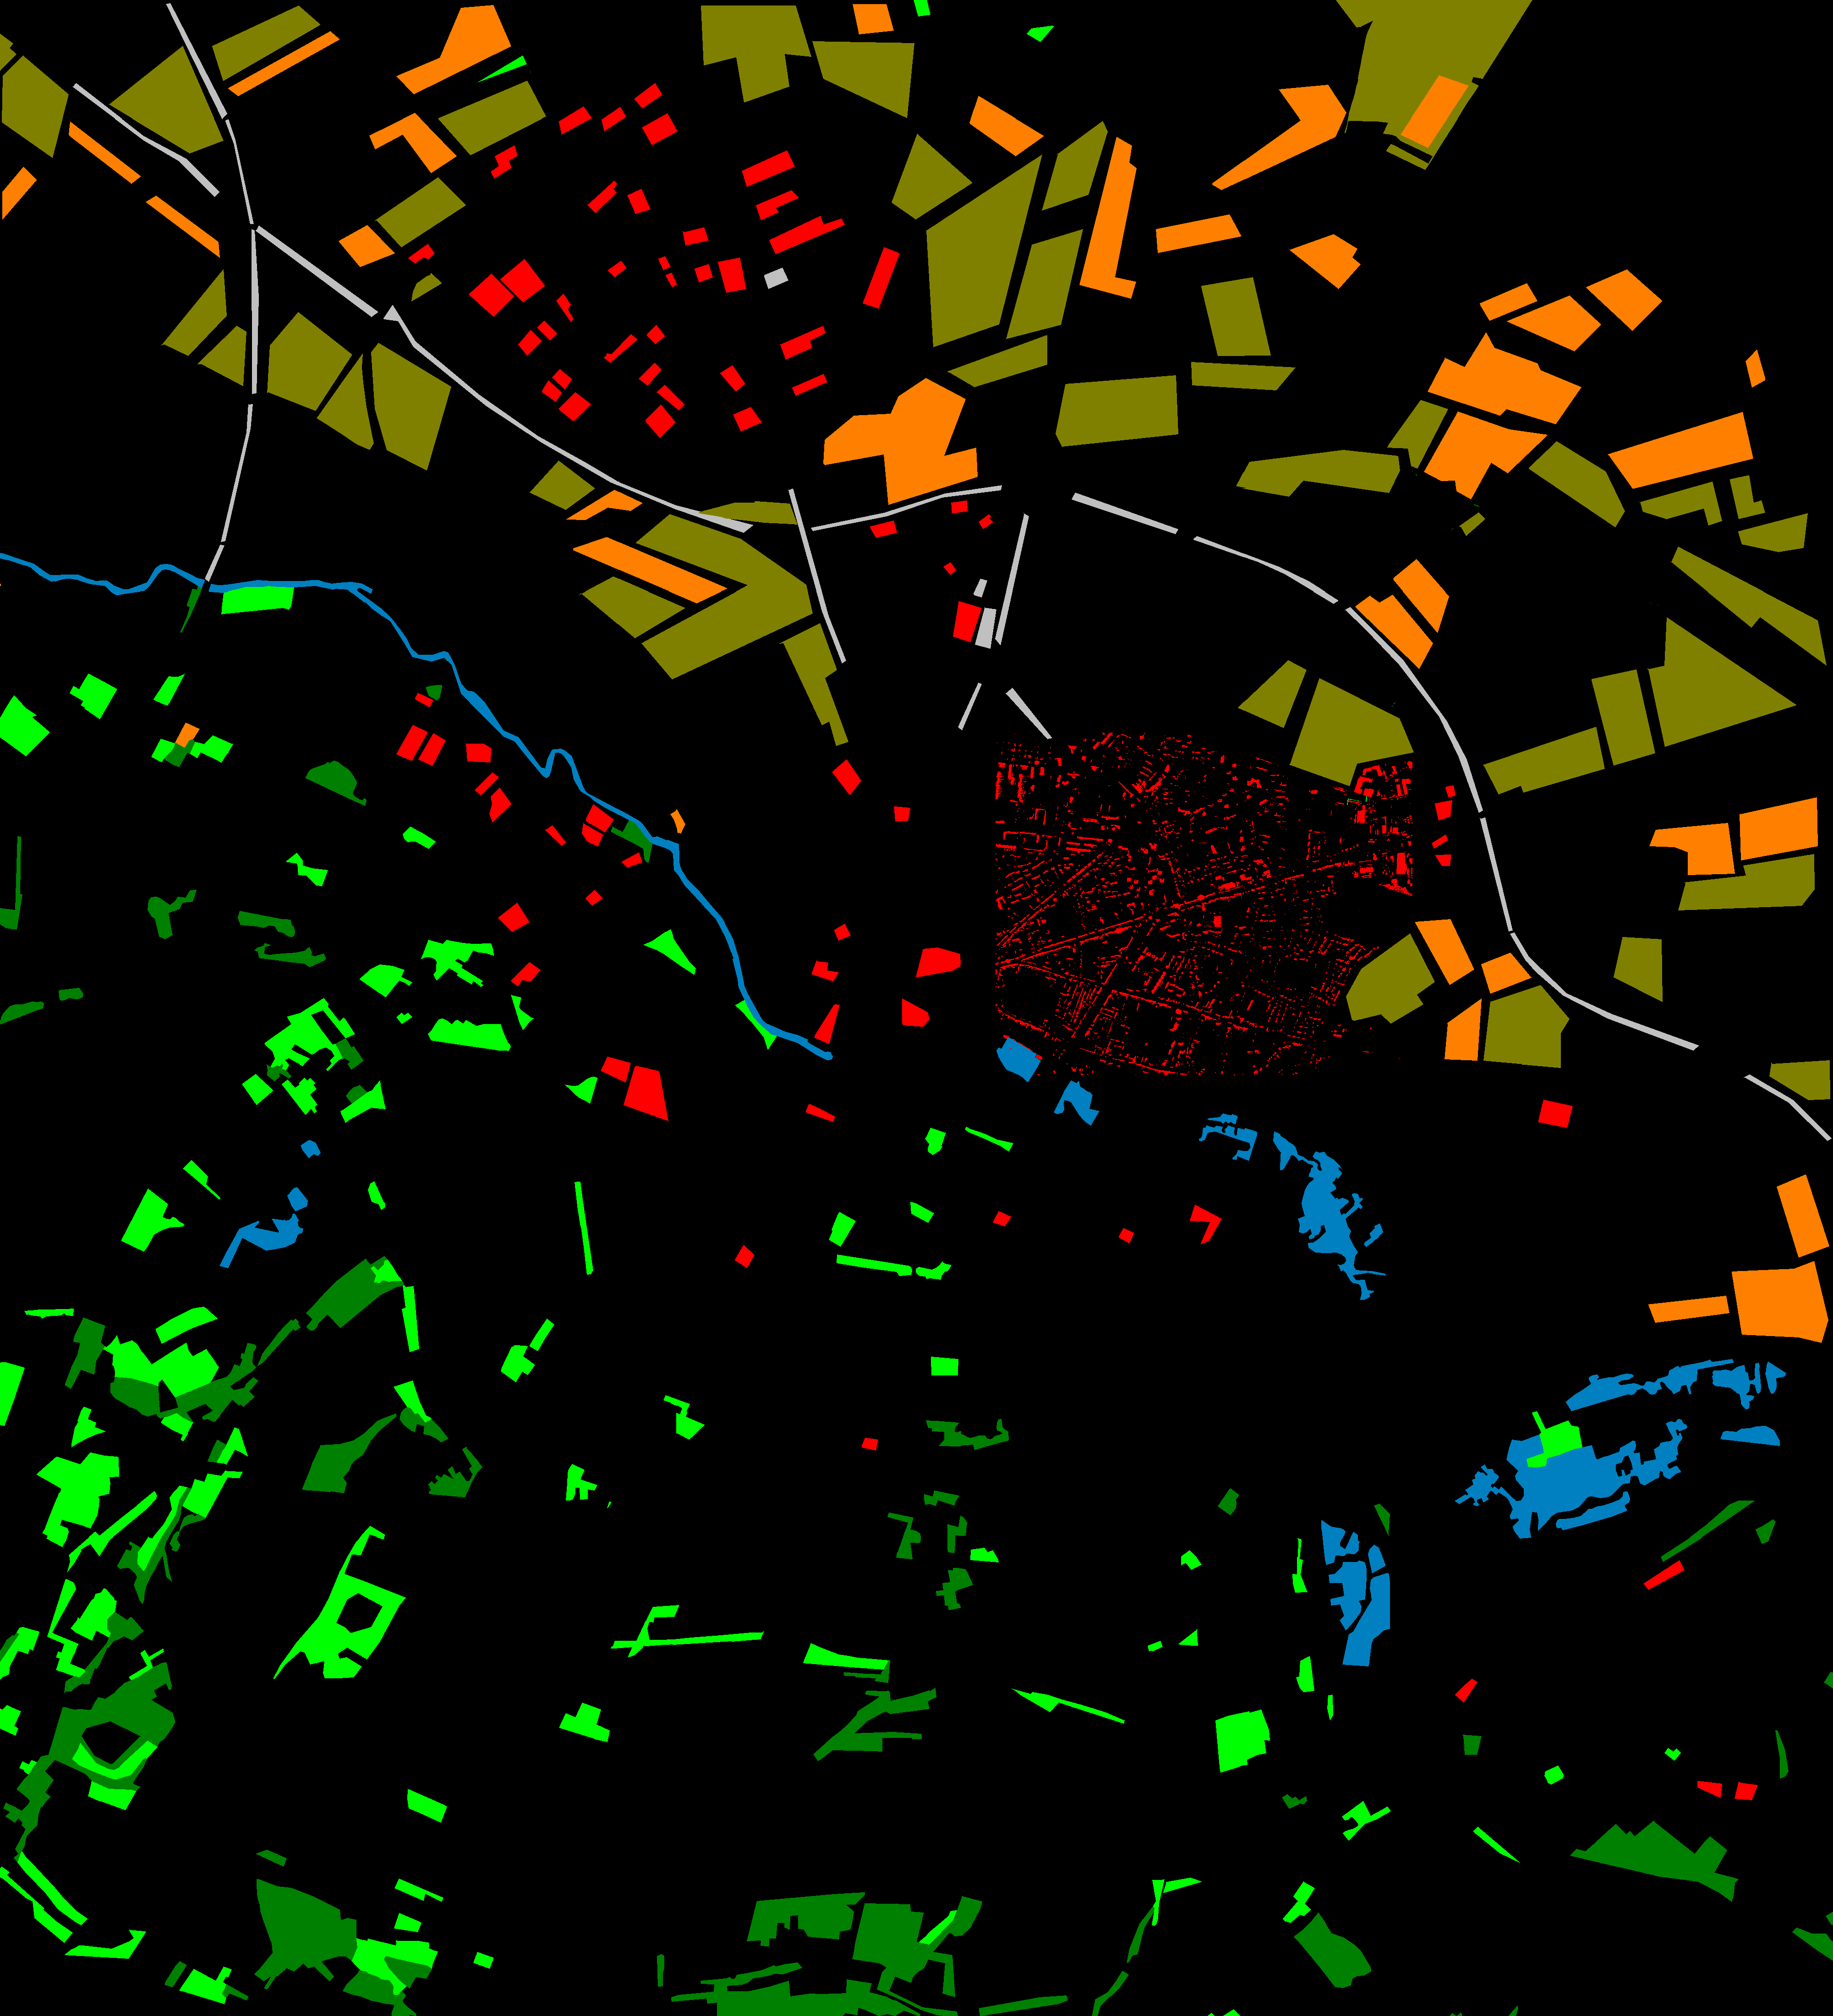
\includegraphics[width=0.4\textwidth]{GT_Amiens2012_2_5m_7classes_TR}}
%     \hspace{4mm}
%    \subfigure[Legenda classi della mappa di \emph{training}]{
%      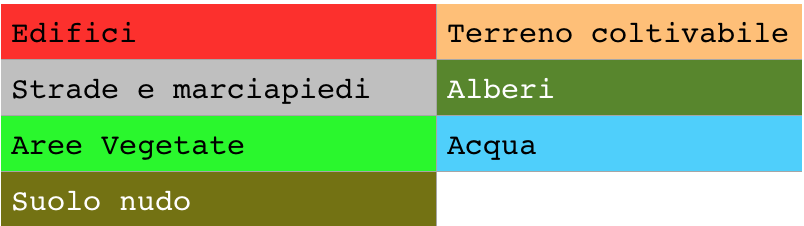
\includegraphics[scale=0.5]{Leggenda_7classi}}
%    \caption{\emph{Dataset} con immagine RBG in falso colore ($4001\times4400$ pixel) acquisita su Amiens (Francia) dal sensore \textsc{SPOT5 HRG} nel 2012}
%    \label{fig: Amiens122_5m}
%  \end{figure}
%\clearpage
%
%\section{Descrizione del classificatore SVM}
%Il classificatore usato è un classificatore \emph{soft-margin} SVM con \emph{kernel} gaussiano. L'implementazione adottata è una variante \emph{ad hoc} della \texttt{LIBSVM} [RIF] scritta in \texttt{C++}.\\
%Il setup utilizzato per la fase di classificazione è composto da un \texttt{MacBookPro Retina} con un processore dual core Intel Core i5 $2.8$ GHz e $16$ GB di memoria e un \texttt{iMac} con processore quad core Intel Core i7 $3.4$ GHz e $8$ GB di memoria. \\
%
%La fase di \emph{training} della SVM, la quale ha complessità temporale $O(n^\alpha)$ ($\alpha$ tipicamente compreso tra 2 e 3) polinomialmente proporzionale al numero di vettori di \emph{training}, ha impiegato, in media, 30 minuti per completare l'ottimizzazione dei parametri, mentre la fase di etichettatura (con complessità $O(n)$ dove $n$ è il numero di vettori da etichettare) ha impiegato, in media, un'ora per esperimento.\\
%L'ottimizzazione dei parametri C e sigma del classificatore è stata effettuata mediante l'applicazione del metodo in [REF] che minimizza un maggiorante sull'errore di generalizzazione del classificatore, detto \emph{"span bound"}, mediante l'algoritmo numerico di Powell.
%
%
%%
%
%\section{Descrizione parametri per estrazione di \emph{feature} di tessitura}
%Qui di seguito verranno presentate le variazioni di accuratezza dell'algoritmo sviluppato al variare delle diverse combinazioni dei parametri in gioco, evidenziando le motivazioni alla base delle scelte progettuali effettuate. La calibrazione dei parametri è stata effettuata sul \emph{dataset} di Amiens 2006-5m\ref{fig: Amiens65m}. 
%
%\subsection{Riduzione del rumore}
%La riduzione del rumore è stata effettuata, come già illustrato in figura \ref{fig:immagine_rumore} nel Capitolo \ref{cap:hog}, tramite un filtraggio passa-basso attraverso un filtro gaussiano bi-dimensionale avente varianza $\sigma$ pari a 2 pixel. Applicando questa gaussiana sia sull'immagine in ingresso all'algoritmo HOG sia sulle immagini HOG risultanti, si opera al fine di ottenere un notevole incremento nella \emph{average accuracy}. In particolare, l'utilizzo di un filtro gaussiano in ingresso aumenta l'AA del $12\%$, mentre l'algoritmo di \emph{noise cleaning} applicato prima e dopo l'estrazione delle \emph{feature} ha fatto registrare un'ulteriore incremento di 2 punti percentuali, portanto l'AA al $14\%$.
%
%\subsection{Calcolo dei gradienti}
%Per quanto riguarda la scelta della maschera da utilizzare per il calcolo del gradiente, sono state valutate diverse opzioni, tra cui la semplice maschera in $1D$ a differenze separate $[-1, 0 ,1]$, la maschera cubica $[1,-8,0,8,-1]$ e filtri  $2D$ più classici come quelli di Prewitt e Sobel.\\
%I risultati migliori sono stati ottenuti con il \emph{kernel} più semplice a $1D$ $3\times1$. Variazioni sulla maschera utilizzata non hanno modificato significativamente i risultati per giustificare un aumento computazionale dovuto all'utilizzo di filtri più complessi.In particolare, con la maschera cubica $5\times5$ l'incremento della AA è stato di appena $+1,5\%$; negli altri casi valutati il risultato è sempre stato peggiore ($-7\%$ con Prewitt e $-3\%con Sobel$.Per questo motivo abbiamo deciso di utilizzare in tutti e tre i casi la soluzione più semplice e ottimale.\\
%
%La direzione del gradiente è stata considerata tra $0$ e $\pi$ (ignorandone quindi il segno) in quanto le strutture geometriche di cui ci interessa avere informazioni (quali strade, fiumi, \ldots) possono essere identificate dalla direzione e non è invece rilevante il verso del gradiente.
%
%\subsection{Numero di canali dei vettori delle \emph{feature}}
%Per quanto riguarda il numero di canali utilizzati per l'istogramma, la scelta che ha fornito prestazioni migliori è risultata essere quella con numero di bande pari a 4. Quantitativamente parlando, i risultati ottenuti con $9$\emph{orientation bins} hanno portato ad un decremento nella AA di $-11\%$. Inoltre, un aumento del numero di \emph{bins} comporta un aumento della risoluzione angolare e, pur apportando complessivamente poca informazione aggiuntiva,  aumenta la dimesionalità dello spazio delle \emph{feature} $\mathbb{R}^d$. Infatti, in primo luogo, all'aumentare di $d$, cresce la complessità computazionale del classificatore, che si traduce in un allungamento dei tempi di calcolo e in una maggiore occupazione di memoria.
%
%\subsection{Dimensione delle celle e dei blocchi}
%La scelta di utilizzare celle di elevate dimensioni introduce un'alta correlazione tra i vettori delle \emph{feature}, mentre un' eccessiva riduzione \textbf{comporta l'inserimento di vettori così scorrelati da avere valori praticamente associabili a rumore.} Un compromesso  è stata trovato empiricamente attraverso diverse sperimentazioni ed è risultato essere diverso (come ci si può aspettare) a seconda della risoluzione spaziale con cui si operava:
%\begin{itemize}
%\item cella da $4\times 4$ pixel, nel caso di pixel di dimensione spaziale pari a 5 m (Figure \ref{fig: Amiens65m})
%\item cella da $2 \times 2$ pixel, nel caso di pixel di dimensione spaziale pari a 2.5 m (Figure \ref{fig: Amiens62_5m} e \ref{fig: Amiens122_5m})
%\end{itemize}
%
%Si è deciso di mantenere costante il numero di pixel usati per la normalizzazione dei blocchi ad un valore di $16\times16$, dal momento che questo valore non inficia la quantità di informazione a disposizione, ma semplicemente normalizza i valori gia calcolati, limitandone l'escursione entro un certo intervallo predefinito.
%
%\clearpage
%
%\section{Discussione dei risultati sperimentali}
%
%\subsection{Amiens 2006 - 5m - 10 classi}
%
%\'E riportata in Figura \ref{fig:ClassMap_Amiens2006_5m} la mappa di
%classificazione con \emph{feature} HOG aggiuntive in configurazione di
%$4$ \emph{bins}, celle di dimensione $4\times4$ pixel e blocchi di
%normalizzazione con $16\times16$ pixel, con filtraggio gaussiano sia
%per l'immagine in ingresso che per le immagini HOG.
%
%\begin{figure}[!ht]
%\center
%\subfigure{
%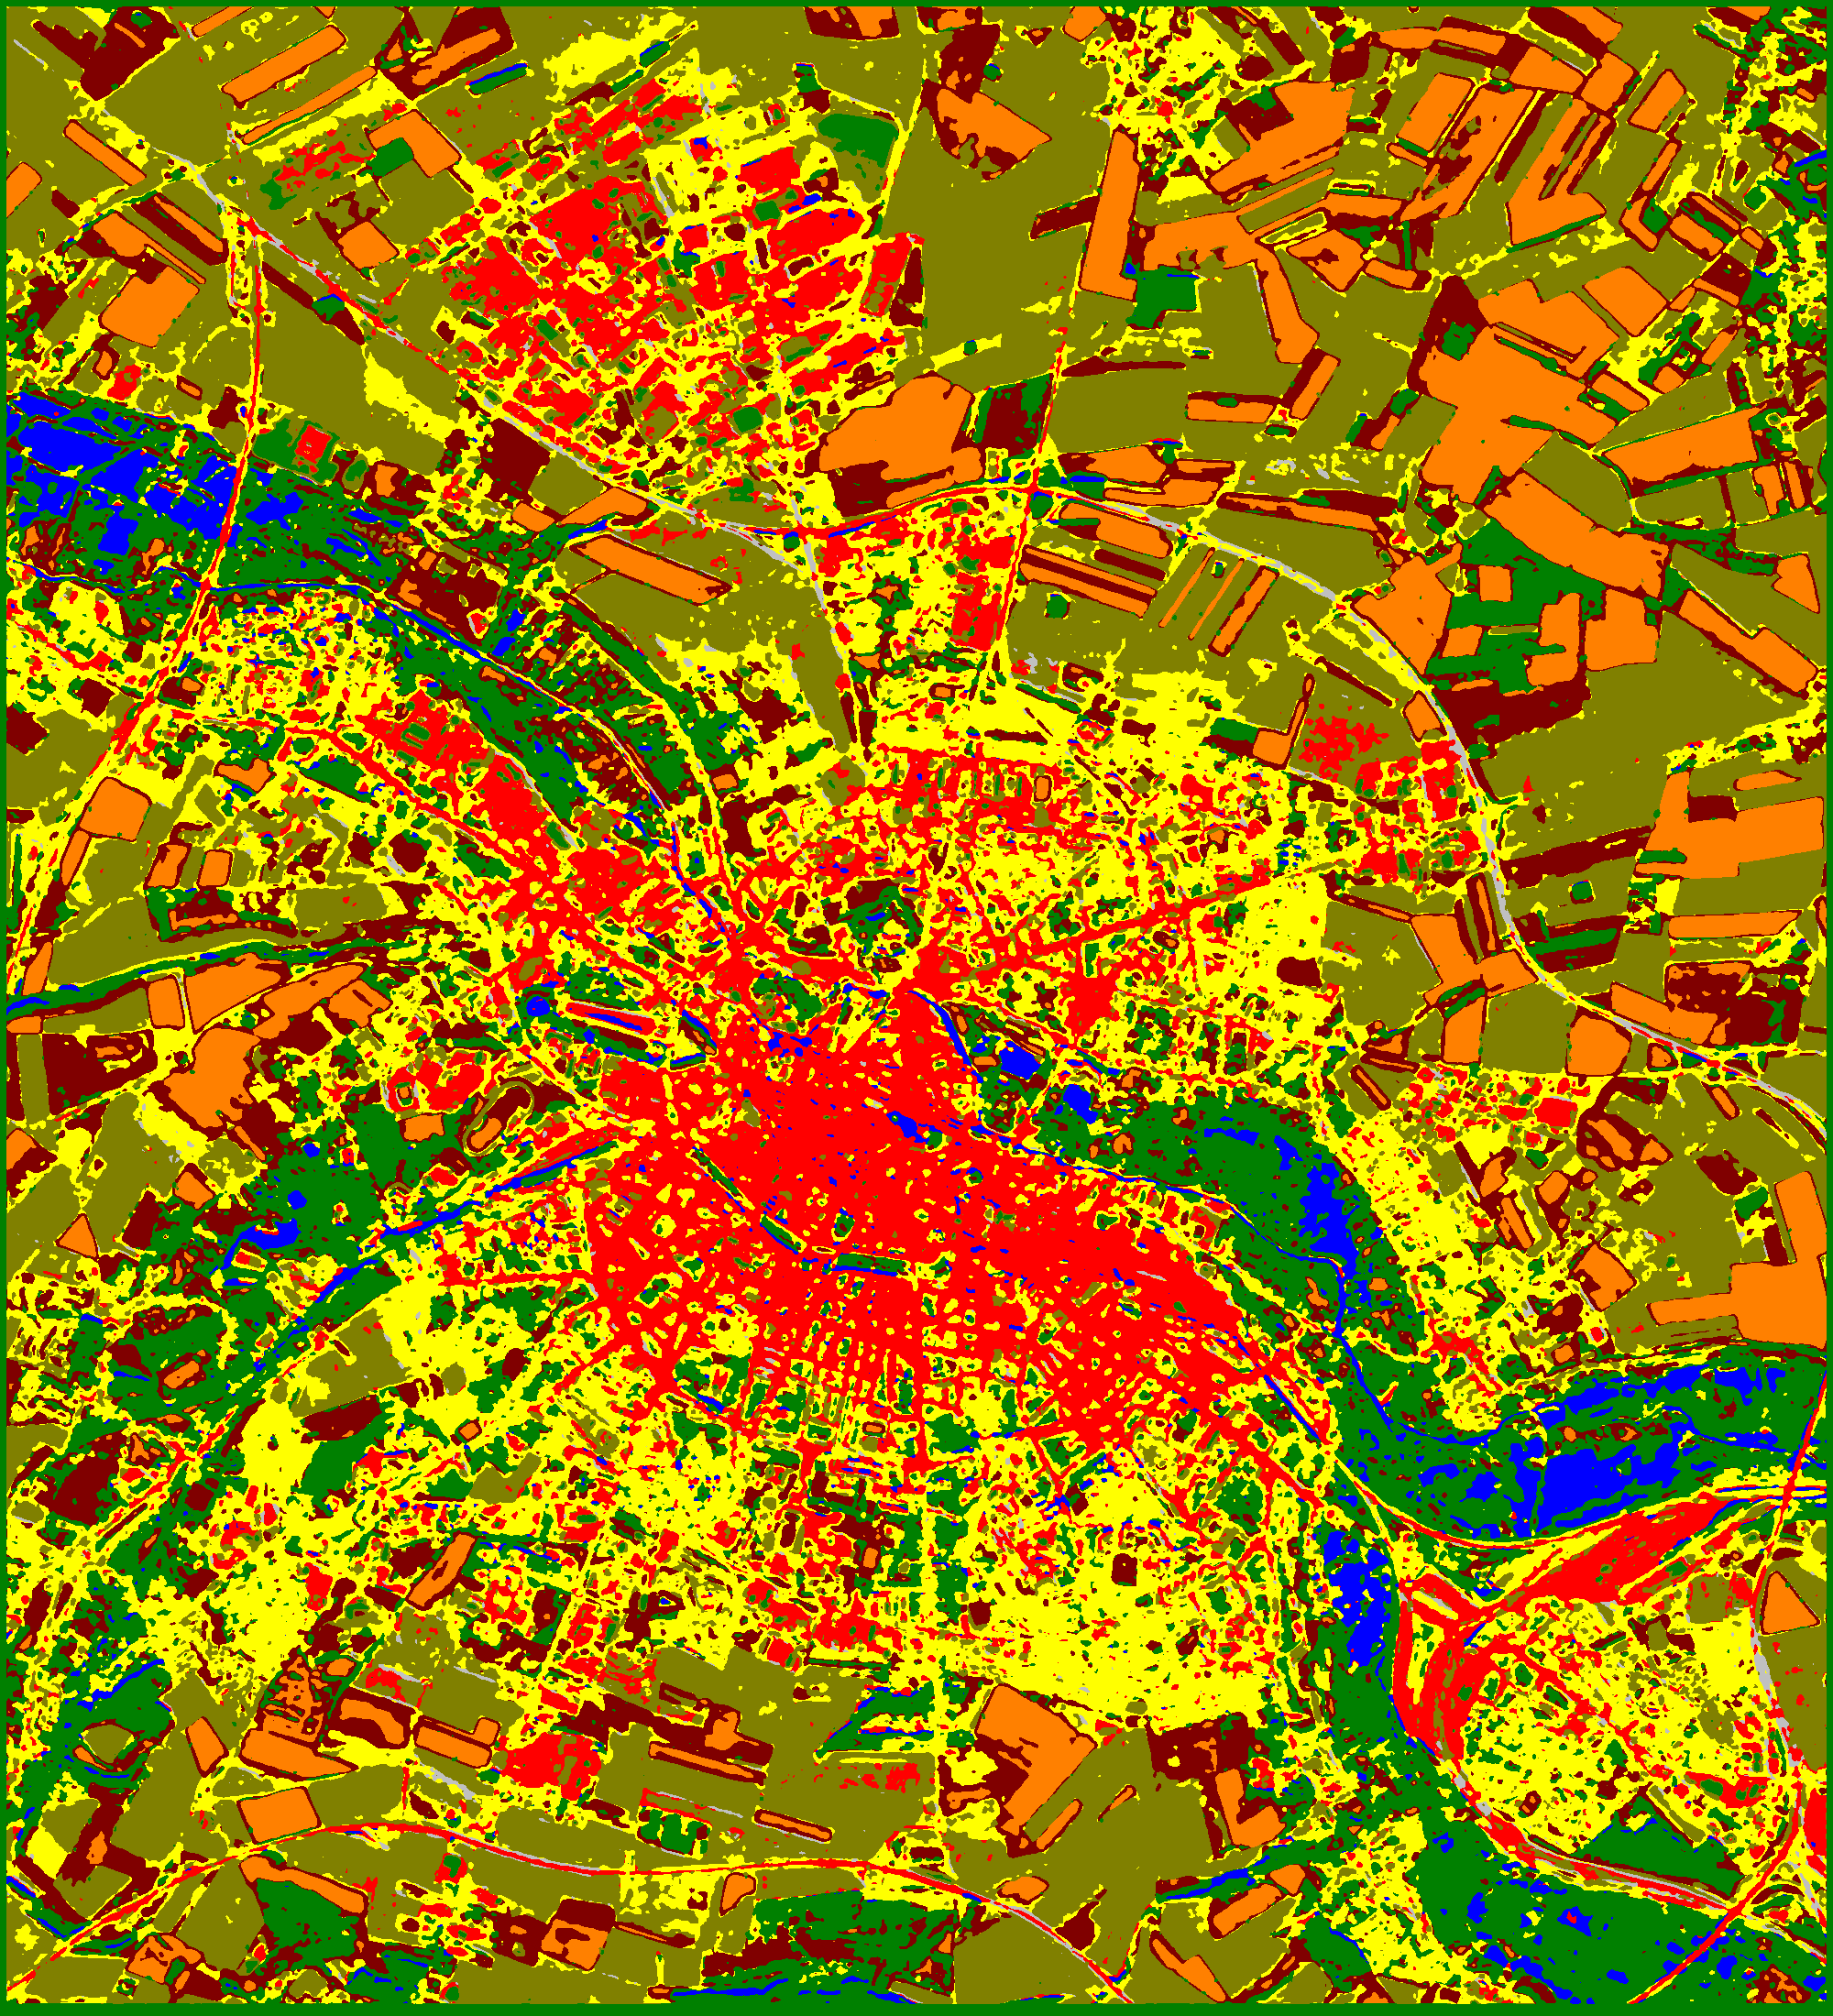
\includegraphics[width=0.7\textwidth]{ClassMap_Amiens2006_5m}}
%\\
%\subfigure{
%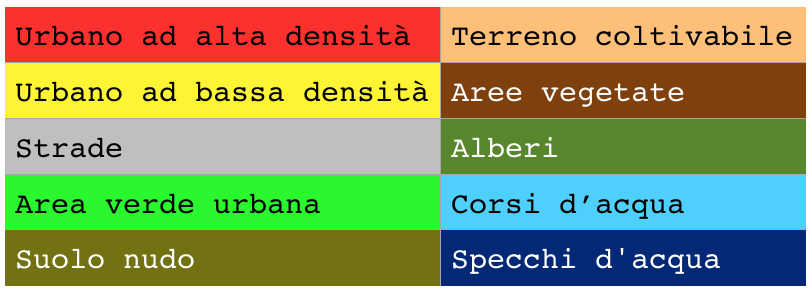
\includegraphics[width=0.35\textwidth]{Leggenda_2006_10classi}}
%
%\caption{Mappa di classificazione del \emph{dataset} \emph{Amiens 2006 - 5m - 10 classi}}
%
%\label{fig:ClassMap_Amiens2006_5m}
%
%\end{figure}
%\clearpage
%Da una prima analisi visiva, si può chiaramente constatare come nel
%complesso la mappa di classificazione sia soddisfacente, sebbene si
%noti già adesso difficoltà nella classificazione delle strade (classe
%3) soprattutto all'interno dell'area urbana. Inoltre, è evidente che
%la classe relativa ai corsi d'acqua (classe 9) non è presente (o
%almeno non apprezzabile).
%
%Sono stati evidenziati, principalmente, due problemi:
%\begin{itemize}
%\item Il primo problema è legato alla risoluzione spaziale dell'immagine in
%ingresso che permette l'identificazione di strade abbstanza larghe, ma
%rende difficoltosa l'identificazione di strade più strette.
%\item Il secondo problema si correla col fatto che il \emph{dataset} include due classi
%associate a corpi idrici: pur rappresentando essi usi del suolo
%differenti, le loro coperture del suolo sono effettivamente analoghe,
%il che ne rende difficile la discriminazione mediante dati
%satellitari, soprattutto caartterizzati da pochi canali spettrali
%(solo tre nel nostro caso).
%\end{itemize}
%
%Queste prime impressioni vengono confermate anche dall'analisi numerica della matrice di confusione (Figura
%\ref{fig:Matrice_di_confusione_Amiens2006_5m_HOG}).
%
%\begin{figure}[!ht]
%
%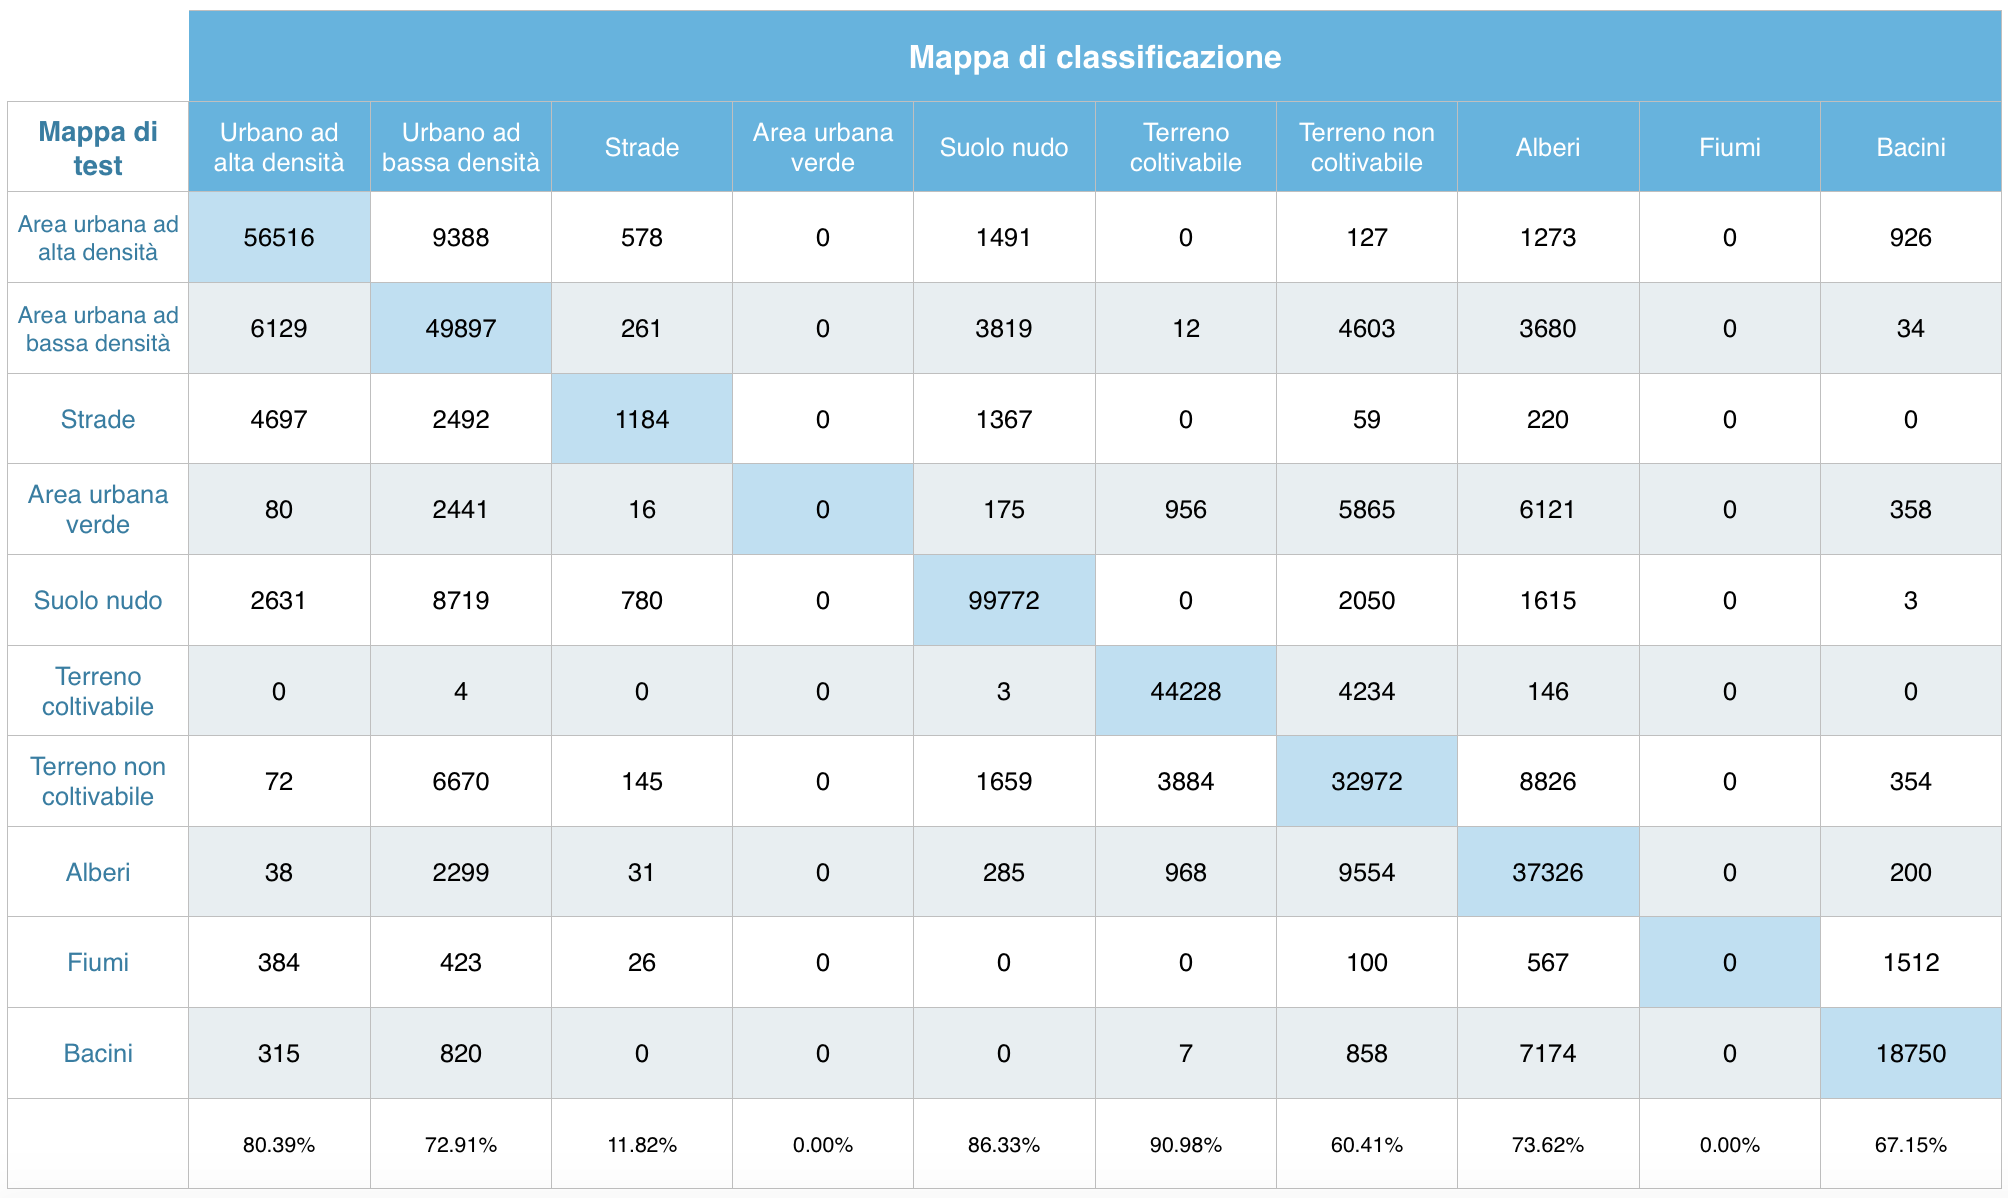
\includegraphics[width=1\textwidth]{Matrice_di_confusione_Amiens2006_5m_HOG}
%
%\caption{Matrice di confusione della sessione di classificazione del
%dataset \emph{Amiens 2006 - 5m - 10 classi}}
%
%\label{fig:Matrice_di_confusione_Amiens2006_5m_HOG}
%
%\end{figure}
%
%Analizzando la matrice di confusione saltano subito all'occhio alcuni
%comportamenti interessanti nella classificazione. La zona urbana
%(classe 1 e 2) viene discriminata in modo soddisfacente (con
%accuratezze nell'ordine del $75\%$); ciò che si perde nell'accuratezza
%deriva in massima parte dalla difficoltà del classificatore di
%distinguere le aree urbane di diversa densità.\\
%
%L'analisi quantitativa della matrice di confusione conferma quanto già
%ipotizzato precedentemente, ovvero che le strade sono quasi del tutto
%perse registrando un'accuratezza di circa $11\%$, a scapito sopratutto
%dell'area urbana. \\
%
%Si è registrata una buona accuratezza nelle classificazioni di aree
%più uniformi quali suolo nudo (classe 5), terreni coltivabili e non
%coltivabile (classi 6 e 7): pochissimi sono i pixel etichettati in
%modo errato per queste regioni, analogamente ai terreni non
%coltivabili, per i quali tuttavia la confusione con la classe "alberi"
%causa accuratezza inferiore.\\
%
%Tuttavia, il classificatore ha avuto serie difficoltà in quelle classi
%minoritarie per le quali il numero di pixel di training era inferiore.
%In particolare, vengono completamente perse l'area verde urbana e i
%corsi d'acqua ($0\%$), le cui etichette sono state assegnate in
%maggioranza alla classe alberi e alla classe bacini d'acqua,
%rispettivamente.\\
%
%Come osservato prima, si tratta di un errore di classificazione dovuto
%alla difficoltà di distinguere classi associate a distinti usi del
%suolo ma sostanzialmente a coperture del suolo molto simili. In
%quest'ottica, il risultato ottenuto si ritiene già soddisfacente.\\
%
%La difficoltà di classificazione di questo \emph{dataset} risiede
%soprattutto nella sovrabbondanza del numero di classi da distinguere,
%in quanto molti errori fatti nella mappa di classificazione sono
%proprio causati dalla confusione di coperture di suolo simili tra
%loro.\\
%
%In termini generali, l'\emph{Overall Accuracy} (OA) complessivo di
%questo primo \emph{dataset} è stato di $73.23\%$, mentre l'AA è
%risultato essere $54.36\%$. Il più basso valore di AA è legato al
%fatto che accuratezze più elevate si siano ottenute per classi
%minoritarie in termini di pixel di test.\\
%
%Per concludere questa prima sessione di discussione, è interessante
%confrontare questi risultati con quelli ottenuti senza estrazione
%delle \emph{feature} HOG. La Figura \ref{fig:Confronto_Amiens2006_5m}
%sintetizza i miglioramenti/peggioramenti classe per classe.
%
%\begin{figure}[!ht]
%
%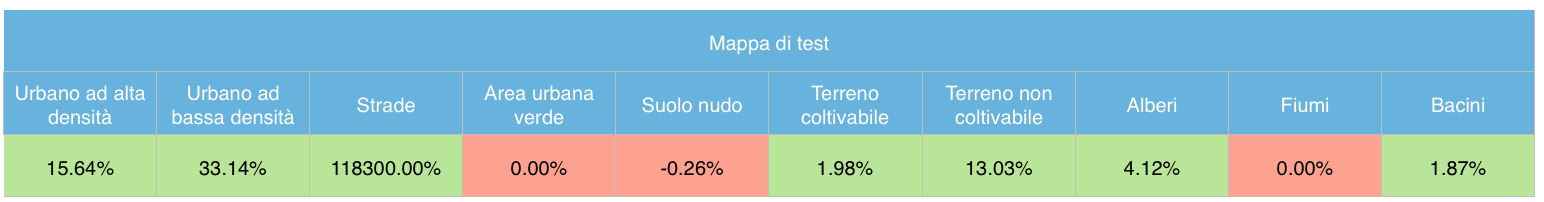
\includegraphics[width=1\textwidth]{Confronto_Amiens2006_5m}
%
%\caption{Confronto percentuale tra accuratezze classe per classe con e
%senza estrazione di \emph{feature}}
%
%\label{fig:Confronto_Amiens2006_5m}
%
%\end{figure}
%
%Si può chiaramente osservare che l'introduzione delle \emph{feature}
%HOG ha quasi sempre apportato miglioramenti, con benefici notevoli
%soprattutto per le classi di suolo urbano. La Figura
%\ref{fig:Confronto_Amiens2006_5m} dimostra come effettivamente il
%risultato della classificazione dell'immagine a tre canali mostri in
%generale più dettaglio; così facendo, però, ciò che si guadagna in
%risoluzione si perde in accuratezza nella classificazione, in quanto
%molti pixel urbani vengono etichettati come appartenenti ad altre
%classi (in particolare la classe 10, gli specchi d'acqua,
%rappresentata in bianco nelle immagini). Il miglioramento ottenuto per
%le classi urbane è coerente con l'informazione direzionale estratta
%dalle feature HOG che risulta utile soprattutto ai fini della
%discriminazione di classi caratterizzate da struttura geometrica.
%
%\begin{figure}[!ht]
%
%\center
%
%\subfigure[Mappa di classificazione con HOG]{
%
%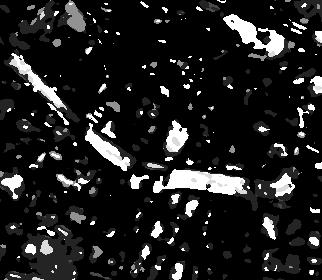
\includegraphics[width=0.4\textwidth]{ClassMap_Amiens2006_5m_HOG}}
%
%\hspace{2mm}
%
%\subfigure[Mappa di classificazione senza HOG]{
%
%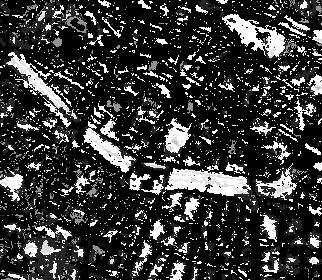
\includegraphics[width=0.4\textwidth]{ClassMap_Amiens2006_5m_riferimento}}
%
%\caption{Confronto su una porzione dell'area urbana di $250\times250$
%pixel della mappa di classificazione con e senza estrazione di
%\emph{feature} HOG sul \emph{dataset} Amiens 2006 a $5$ m(il nero rappresenta gli "edifici", mentre i pixel bianchi corrispondono alla classe "acqua")}
%
%\label{fig:confrontoAmiens2006_5m}
%
%\end{figure}
%
%\clearpage
%
%%\subsection{Amiens 2006 - 2.5m - 7 classi}
%
%%Come già introdotto nel caso precedente, anche per questo esperimento
%
%%foto-interpretativa
%
%%\clearpage
%
%\subsection{Amiens 2012 - 2.5m - 7 classi}
%
%\'E riportata in Figura \ref{fig:ClassMap_Amiens2012_2_5m_noroads} la
%mappa di classificazione con \emph{feature} HOG, in aggiunta alle tre
%feature spettrali, in configurazione di $4$ \emph{bins}, celle di
%dimensione $2\times2$ pixel e blocchi di normalizzazione con
%$16\times16$ pixel, con filtraggio gaussiano sia per l'immagine in
%ingresso che per le immagini HOG.
%
%\begin{figure}[!ht]
%
%\center
%
%\subfigure{
%
%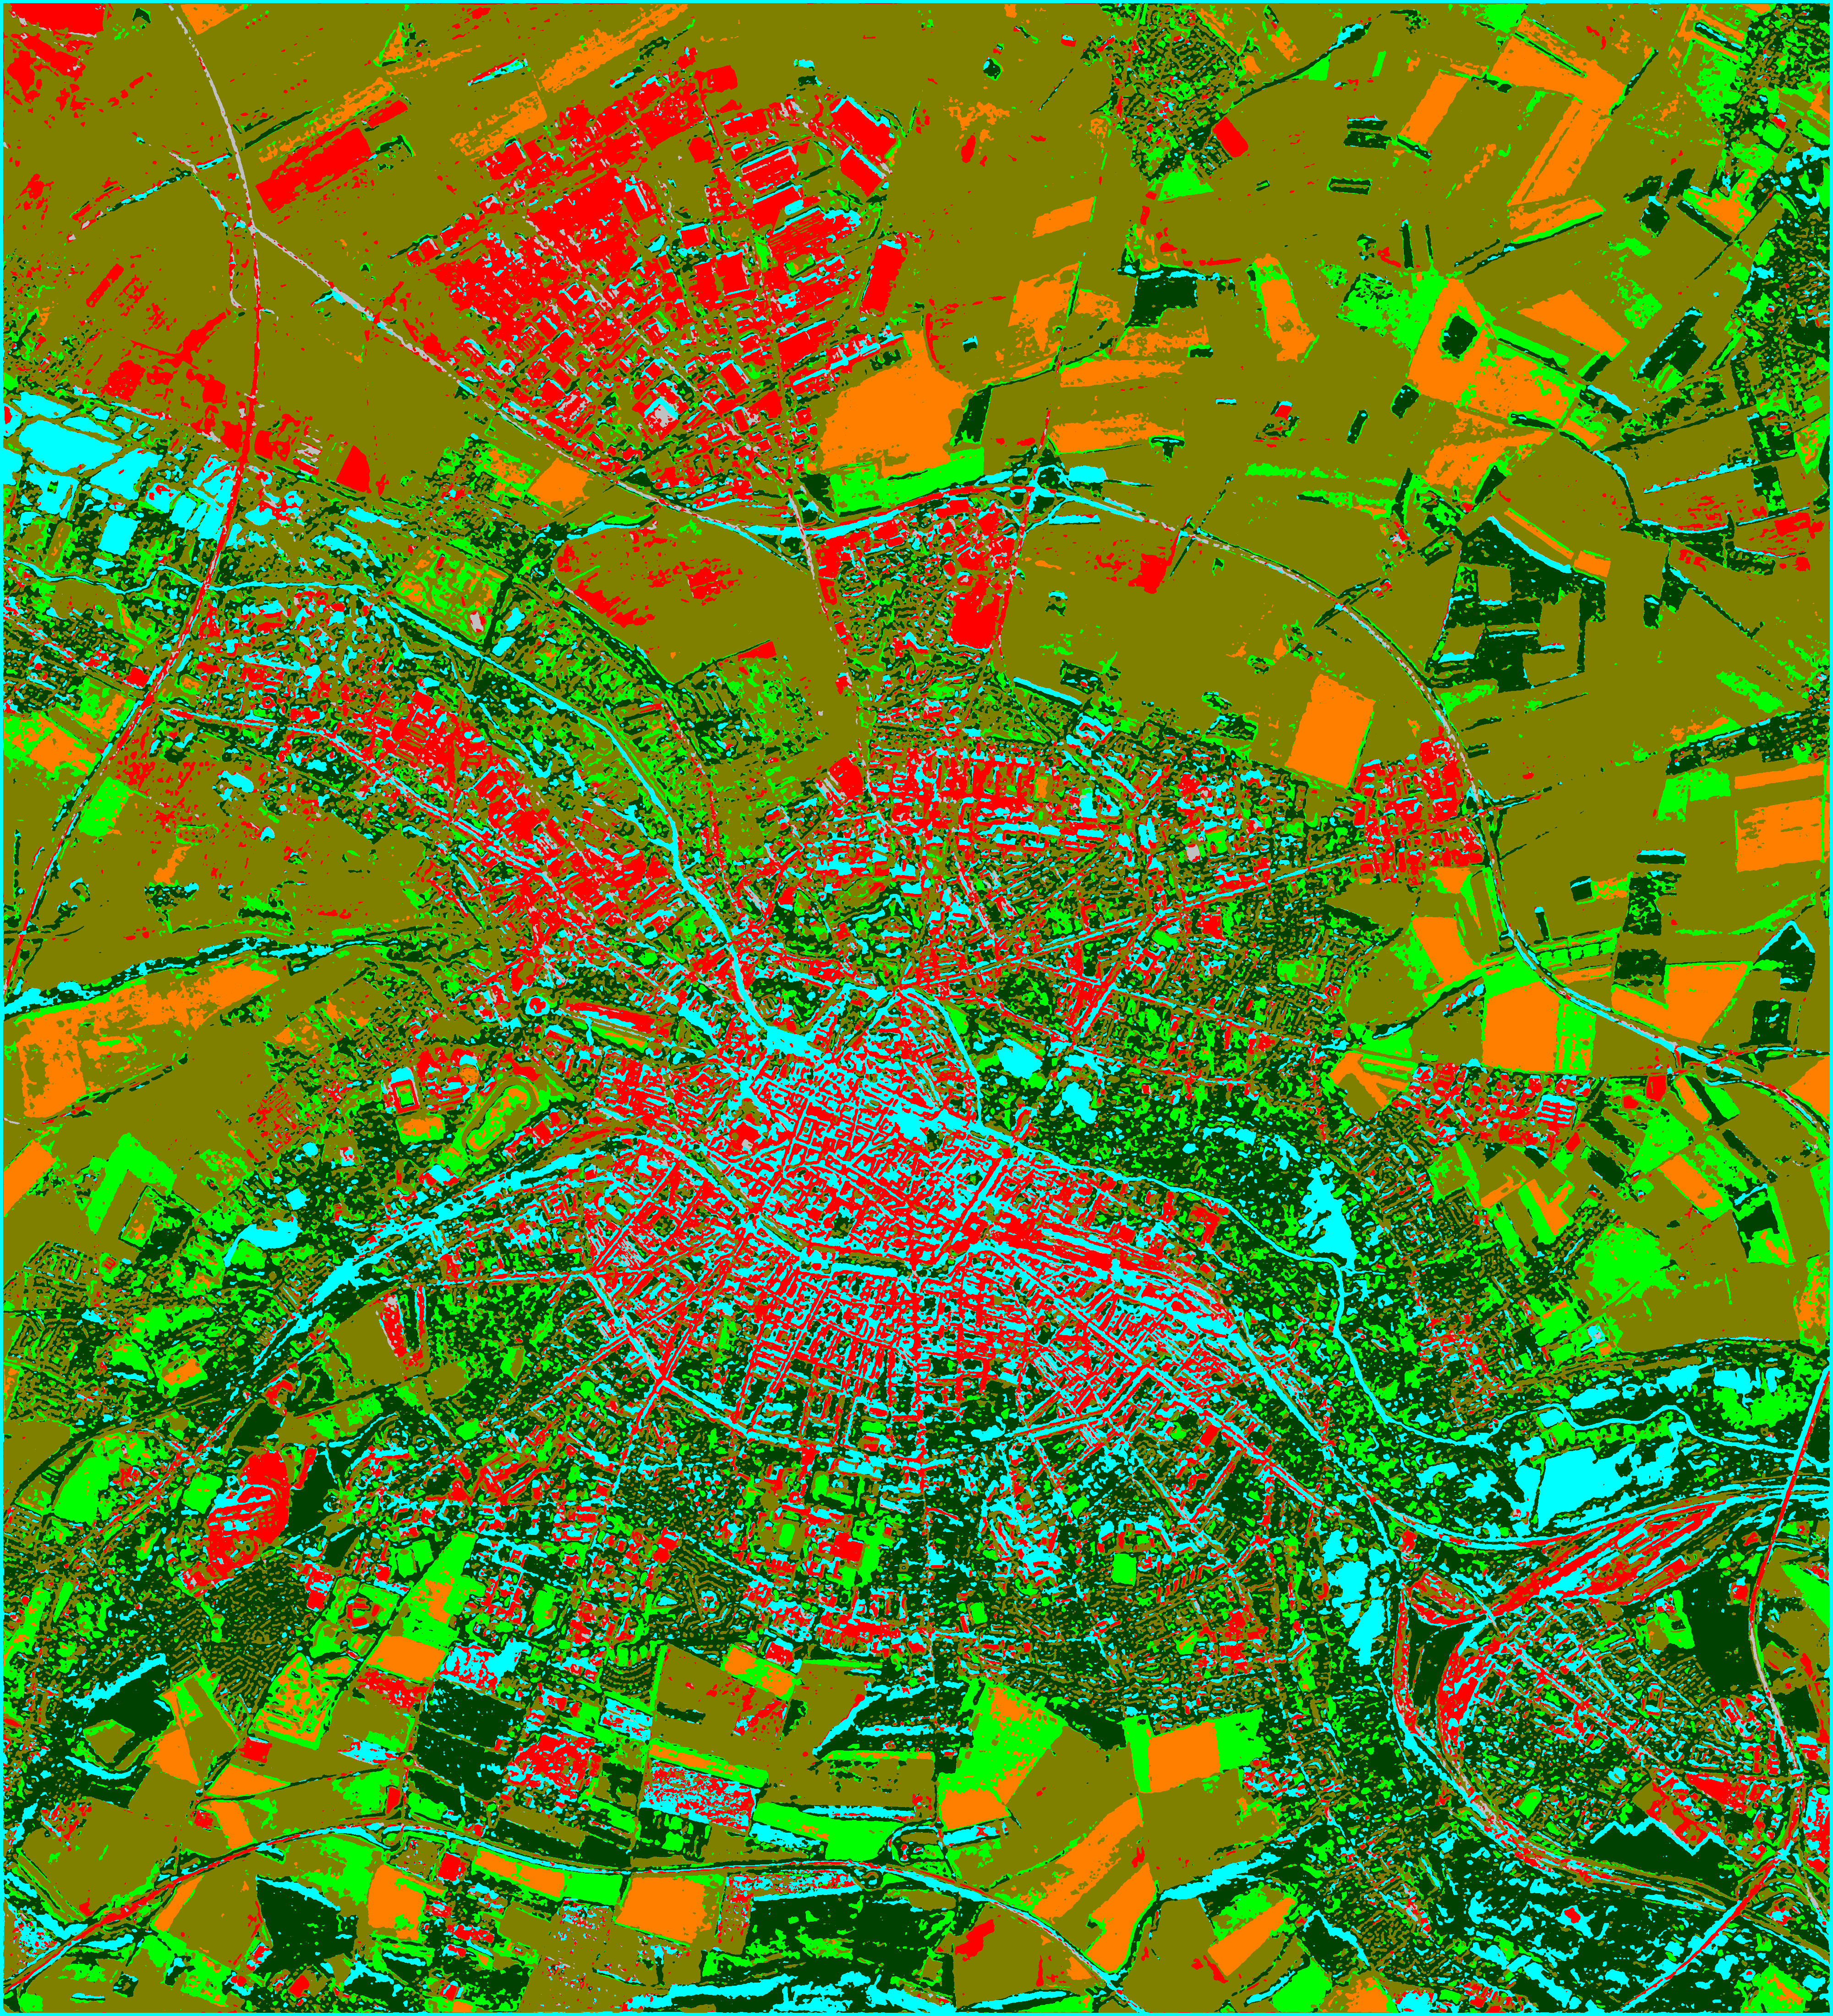
\includegraphics[width=0.7\textwidth]{ClassMap_Amiens2012_2_5m_noroads}}
%\\
%\subfigure{
%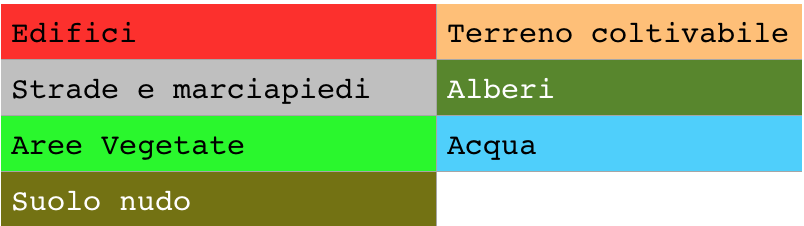
\includegraphics[width=0.35\textwidth]{Leggenda_7classi}}
%
%\caption{Mappa di classificazione del dataset \emph{Amiens 2012 - 2.5m
%- 7 classi}}
%
%\label{fig:ClassMap_Amiens2012_2_5m_noroads}
%
%\end{figure}
%\clearpage
%\'E importante far notare fin da subito che l'immagine telerilevata
%che fa parte di questo \emph{dataset} è stata acquisita in situazioni
%ambientali e in periodi di tempo diversi da quelle precedenti
%(nell'inverno 2012). Questo costituisce un evidente deficit
%nell'informazione proveniente dal suolo, in quanto la stagione di
%acquisizione ha reso altamente più complesso la discriminazione delle
%7 diverse coperture di suolo. Le classi vegetate, in particolare,
%corrispondono qui a coperture del suolo che presentano similarità col
%suolo nudo, avendo l'acquisizione avuto luogo in un periodo dell'anno
%in cui gli alberi avevano perso le foglie e le aree agricole non
%presentavano gia più vegetazione coltivata evidente.\\
%
%Già con un'analisi della mappa, si osserva che qualitativamente il
%risultato sembra peggiorare rispetto all'esperimento precedente. Due
%sono i punti critici già a prima vista apprezzabili:
%
%\begin{itemize}
%
%\item i pixel etichettati come appartenenti al suolo nudo (classe 4)
%sembrano essere in misura sovrabbondante rispetto ai risultati precedenti: ciò
%può essere giustificato dal commento precedente;
%
%\item la quasi totale scomparsa delle strade (classe 2) nel centro,
%che talora vengono classificate come pixel appartenenti alla classe
%acqua (classe 7). Ciò si spiega non solo in relazione alla risoluzione
%spaziale dell'immagine considerata ma anche col fatto che molte strade
%presentino ombre di alcuni edifici; soprattutto quando osservata con
%tre soli canali, la risposta spettrale delle zone in ombra si presenta
%molto simile a quella dei corpi idrici.
%
%\end{itemize}
%
%Queste considerazioni trovano conferma negli indici di accuratezza che
%raggiungono, in assoluto, valori meno soddisfacenti rispetto ai casi
%esaminati in precedenza.
%
%L'OA per questo esperimento, infatti, si è fermata al $56.63\%$,
%mentre l'AA ha raggiunto il valore di $57.33\%$.\\
%
%In Figura \ref{fig:Matrice_di_confusione_Amiens2012_5m_HOG_without_roads}
%viene presentata la matrice di confusione di questo esperimento. \\
%
%\begin{figure}[!ht]
%
%\includegraphics[width=1\textwidth]{Matrice_di_confusione_Amiens2012_5m_HOG_without_roads}
%
%\caption{Matrice di confusione della sessione di classificazione del
%\emph{dataset} \emph{Amiens 2012 - 5m - 7 classi}}
%
%\label{fig:Matrice_di_confusione_Amiens2012_5m_HOG_without_roads}
%\end{figure}
%
%Si può osservare che la classe per la quale la classificazione ha
%ottenuto i risultati migliori è stata quella relativa al terreno
%coltivabile (classe 5), che ha registrato un accuratezza di oltre il $90\%$.
%Prestazioni soddisfacenti sono state raggiunte anche per le classi di
%suolo nudo e acqua (classi 4 e 7), in cui una buona percentuale di
%pixel della mappa di classificazione coincide con la verità al
%suolo.\\
%
% \begin{figure}[!ht]
%
%\center
%
% \subfigure[Mappa di classificazione senza HOG]{
%
% \includegraphics[width=0.4\textwidth]{ClassMap_Amiens2012_2_5m_riferimento}
%
% }
%
% \hspace{3mm}
%
% \subfigure[Mappa di classificazione con HOG]{
%
% \includegraphics[width=0.4\textwidth]{ClassMap_Amiens2012_2_5m_HOG}
% } \caption{Confronto su una porzione dell'area urbana di
%$250\times250$ pixel della mappa di classificazione con e senza
%estrazione di \emph{feature} HOG sul \emph{dataset} Amiens 2012 a
%$2.5$ m }
% \label{fig:confrontoAmiens2012_2_5m}
%\end{figure}
%
%\begin{figure}[!ht]
%
%\includegraphics[width=1\textwidth]{Confronto_Amiens2012_con_e_senza_hog}
%
%\caption{Confronto percentuale tra accuratezze classe per classe con e
%senza estrazione di \emph{feature} per il \emph{dataset} Amiens 2012 a
%$2.5$ m}
%
%\label{fig:Confronto_Amiens2012_2.5m}
%
%\end{figure}
%
%Confrontando i risultati ottenuti dalla classificazione con HOG e da
%quella avente come \emph{feature} le sole tre bande telerilevate, si
%osserva come, anche questa volta, l'introduzione degli HOG porti, in
%generale, ad un incremento della percentuale di pixel classificati
%correttamente: in particolare in Figura
%\ref{fig:Confronto_Amiens2012_2.5m} si può notare un netto
%miglioramento ($+2537\%$) per le strade, benché in termini assoluti
%restino ancora ben poco classificate ($10\%$) probabilmente a causa
%della presenza di ombre . Si è rilevato, tuttavia, un leggero
%peggioramento ($-16\%$) nell' individuazione degli edifici. \\ In
%conclusione, la presenza degli HOG migliora anche OA e AA seppure in
%maniera limitata. \\
%
%Vista la non ancora soddisfacente percentuale di pixel di strada
%classificati in maniera adeguata, si è deciso di inserire una
%\emph{feature} aggiuntiva della struttura cartografica delle strade di
%Amiens. L'immagine binaria in Figura \ref{fig:immagine_roads} è stata
%inserita nel vettore delle \emph{feature} in coda all'immagine
%precedente con vettori HOG.
%
%Quest'immagine è il risultato della fusione di tre mappe tematiche
%(strade principali, strade secondarie e binari ferroviari, riportati
%unitamente a parte del territorio circostante quando tale territorio
%non presenti altro uso che quello associato ai trasporti), ottenuta
%dal servizio di mappatura stradale della European Urban Atlas. In
%particolare, l'immagine è aggiornata all'anno $2006$ e possiede una
%risoluzione spaziale di 5 m/pixel.
%
%%\begin{figure}[!ht]
%%
%%\center
%%
%%\includegraphics[width=0.8\textwidth]{amiens6_roads}
%%
%%\caption{Immagine binaria della struttura cartografica delle strade di
%%Amiens: le strade sono rappresentate con il bianco e lo sfondo in
%%nero.}
%%
%%\label{fig:immagine_roads}
%%
%%\end{figure}
%
%In questo modo, si è riusciti a limitare la degradazione della classe
%strade (classe 2) portandola ad un più che accettabile valore di
%accuratezza ($64.61\%$); dal momento che il numero di pixel
%classificati come strade non è molto significativo nella totalità dei
%pixel dell'immagine, non si ha un'apprezzabile incremento dell'OA,
%al
%contrario della AA che, pesando gli errori uniformemente, registra un
%significativo miglioramento ($63.54\%$).
%
%In Figura \ref{fig:confrontoAmiens2012_2_5m} viene mostrato l'effetto
%di questa \emph{feature} aggiuntiva per la classificazione delle
%strade.
%
%% (la porzione di immagine utilizzata è la stessa della Figura
%%\ref{fig:confrontoAmiens2012_2_5m}, per una più immediata
%%comprensione).
%
%\begin{figure}[!ht]
%\center
%\subfigure[Mappa di classificazione senza HOG]{
%\includegraphics[width=0.35\textwidth]{ClassMap_Amiens2012_2_5m_riferimento}
%}
%\hspace{3mm}
%\subfigure[Mappa di classificazione con HOG]{
%\includegraphics[width=0.35\textwidth]{ClassMap_Amiens2012_2_5m_HOG}
%}
%\\
%\subfigure[Mappa di classificazione con HOG e cartografia]{
%\includegraphics[width=0.35\textwidth]{ClassMap_Amiens2012_2_5m_HOG_and_roads}
%}
%\caption{Confronto su una porzione della periferia di Amiens di
%$250\times250$ pixel della mappa di classificazione con e senza
%estrazione di \emph{feature} HOG e con l'aggiunta della cartografia
%stradale sul \emph{dataset} Amiens 2012 a $2.5$ m. }
%\label{fig:confrontoAmiens2012_2_5m}
%\end{figure}
%
%\clearpage
%
%\subsection{Amiens 2006 - 2.5m - 7 classi}
%
%\'E riportata in Figura \ref{fig:ClassMap_Amiens2006_2_5m_roadsandhog}
%la mappa di classificazione con \emph{feature} HOG aggiuntive in
%configurazione di $4$ \emph{bins}, celle di dimensione $2\times2$
%pixel e blocchi di normalizzazione con $16\times16$ pixel, con
%filtraggio gaussiano sia per l'immagine in ingresso che per le
%immagini HOG e con l'aggiunta della \emph{feature} cartografica delle
%strade di Amiens.
%
%\begin{figure}[!ht]
%
%\center
%\subfigure{
%\includegraphics[width=0.7\textwidth]{ClassMap_Amiens2006_2_5m_roadsandhog}}
%\\
%\subfigure{
%
%\includegraphics[width=0.35\textwidth]{Leggenda_7classi}}
%
%\caption{Mappa di classificazione del dataset \emph{Amiens 2006 - 2.5m
%- 7 classi}}
%
%\label{fig:ClassMap_Amiens2006_2_5m_roadsandhog}
%
%\end{figure}
%
%Su questo \emph{dataset} i risultati sono stati interessanti, poichè
%si differenziano notevolmente dai due casi studiati in precedenza.\\
%
%E' innanzitutto importante far notare che questo esperimento ha
%registrato il valore più alto a livello di OA ($74.88\%$) e AA
%($70.61\%$). \\
%
%L'analisi della matrice di confusione (riportata in Figura
%\ref{fig:ClassMap_Amiens2006_2_5m_roadsandhog}) conferma il fatto che
%il classificatore, per questo \emph{dataset}, si comporti mediamente
%bene su tutte le classi, presentando accuratezze abbastanza elevate,
%soprattutto in rapporto alla difficoltà del problema di
%classificazione affrontato, per tutte le 7 classi presenti.\\L'unico
%caso in cui i risultati non sono del tutto accettabili riguarda la
%distinzione tra area vegetata (classe 3) e alberi (classe 6), i cui
%pixel vengono spesso confusi tra le due categorie.
%
%\begin{figure}[!ht]
%
%\includegraphics[width=1\textwidth]{Matrice_di_confusione_Amiens2006_2_5m_HOG_and_roads}
%
%\caption{Mappa di classificazione del dataset \emph{Amiens 2006 - 2.5m
%- 7 classi}}
%
%\label{fig:Matrice_di_confusione_Amiens2006_2_5m_HOG_and_roads}
%
%\end{figure}
%
%In Figura \ref{fig:Confronto_Amiens2006_2_5m_con_e_senza_hog_e_roads}
%vengono proposte le variazioni di prestazioni classe per classe nel
%confronto fra questo risultato e quello ottenuto senza feature HOG.\\
%
%\begin{figure}[!ht]
%
%\includegraphics[width=1\textwidth]{Confronto_Amiens2006_2_5m_con_e_senza_hog_e_roads}
%
%\caption{Confronto percentuale tra accuratezze classe per classe con e
%senza estrazione di \emph{feature} per il \emph{dataset} Amiens 2006 a
%$2.5$ m}
%
%\label{fig:Confronto_Amiens2006_2_5m_con_e_senza_hog_e_roads}
%
%\end{figure}
%
%Si osserva come l'introduzione delle \emph{feature} HOG peggiora quasi
%tutti i valori di precisione del classificatore.\\
%
%Tuttavia, come era possibile ipotizzare già dopo l'analisi dei due
%precedenti esperimenti, l'uso di \emph{HOG}, unito all'aggiunta della
%mappa cartografica, permette di far registrare un incremento notevole
%alla classe deputata all'etichettatura delle strade, che senza HOG è
%sempre la classe che registra i livelli di accuratezza più bassi,
%spesso insufficienti a dare una buona rappresentazione della verità al
%suolo. Tale risultato, insieme con quelli osservati in riferimento
%agli altri due data set, suggerisce come l'uso di HOG in un problema
%di classificazione a risoluzione spaziale abbastanza elevata in aree
%urbane presenti benefici in termini di capacità di discriminazione di
%classi con struttura geometrica ben definita, ma anche potenziali
%svantaggi, soprattutto in riferimento all'identificazione di classi
%prive di tale struttura a causa della loro natura fisica (ad es.,
%alberi) o delle condizioni di acquisizione (ad es., sfocatura nei dati
%o presenza di ombre).
%
%%%!TEX root = ../main.tex
%%
%%\chapter{Valutazione delle prestazioni del classificatore}
%%\label{cap:prestazioni}
%%
%%Dato un classificatore supervisionato, addestrato su un \emph{training set}, è fondamentale saper valutare l'accuratezza che può essere ottenuta quando tale classificatore è applicato a campioni incogniti.\\
%%A tale scopo, è essenziale valutare la probabilità di errore $P_e$ del classificatore per decidere, ad esempio, se le \emph{feature} utilizzate siano sufficienti a discriminare bene le classi o se sia necessario estrarne altre (come parametri di tessitura nel caso in cui i canali spettrali non siano abbastanza discriminanti).
%%\clearpage
%%
%%\subsection{Stima della probabilità di errore}
%%In presenza di $C$ classi $\omega_1,\omega_2, \ldots, \omega_C$, detta $P_i$ la probabilità \emph{a priori}, la probabilità di errore $P_e$ si può esprimere nel modo seguente:
%%\begin{equation}
%%\label{eq:P_e}
%%P_e = P\lbrace\widehat{Y}\neq Y\rbrace= {\sum_{i=1}^C P\lbrace\widehat{Y}\neq \omega_i\vert Y = \omega_i\rbrace}P\lbrace Y =\omega_i\rbrace
%%\end{equation}
%%dove $Y$ è l'etichetta di classe corrispondente alla realtà a terra e $\hat{Y}$ è l'etichetta stimata dal classificatore.
%%Dal momento che tale espressione è calcolabile solo in pochissimi casi semplici, per valutarla si adotta generalmente un approccio empirico, che stima la $P_e$ come la percentuale dei pixel di test classificati erroneamente.\\
%%Solitamente la $P_e$ viene valutata su un insieme di campioni pre-etichettati(\emph{test set}) diverso rispetto a quello utilizzato per addestrare il classificatore(\emph{training set}). Questa tecnica, detta \emph{hold-out}, permette una misura delle prestazioni priva di \emph{bias} in quanto eseguita su istanze non utilizzate in fase di apprendimento.\\
%%Per poter individuare e possibilmente evitare il fenomeno dell'\emph{overfitting},\footnote{Si parla di \emph{overfitting} quando la funzione discriminante è strettamente dipendente dai campioni di \emph{training} specifici utilizzati per calcolarla ed è quindi particolarmente inefficace quando applicata a campioni incogniti} una condizione fondamentale per stimare $P_e$ come frequenza relativa degli errori sul \emph{test set} è che i campioni pre-etichettati siano indipendenti e identicamente distribuiti (i.i.d). Per questa ragione, è buona norma prelevare i campioni di \emph{training} e di \emph{test} in regioni dell'immagine spazialmente disgiunte tra loro.\\
%%E' altrettanto importante effettuare un'analisi qualitativa dell'intera mappa, mediante foto-interpretazione, come complemento alla valutazione quantitativa delle prestazioni di classificazione sui campioni di test.
%%
%%\subsection{Matrice di confusione e parametri di accuratezza}
%%La $P_e$ fornisce una valutazione complessiva delle prestazioni del classificatore, senza però differenziare gli errori commessi in corrispondenza di classi diverse. Per una valutazione più dettagliata la matrice di confusione (\emph{confusion matrix}) è la tipologia di osservazione statistica maggiormente utilizzata: il risultato della classificazione sulle aree campione viene confrontato con la verità al suolo [Congalton]. Questa è una matrice $C \times C$, il cui elemento $e_{ij}$ è il numero di pixel di test della classe $\omega_i$ che il classificatore ha assegnato alla classe $\omega_j$. Sulla diagonale $i=j$ della matrice di confusione si leggono dunque i numeri di pixel di test classificati in modo corretto. Questo tipo di analisi statistica consente non solo di quantificare il successo ottenuto dalla procedura, ma anche di focalizzare i punti critici del processo di classificazione, ovvero le classi meno distinguibili tra loro. \\
%%L'accuratezza della classificazione può essere valutata con diversi parametri numerici, tra cui i più utilizzati sono i seguenti:
%%\begin{itemize}
%%\item La \emph{Producer Accuracy} (PA) di una classe $\omega_i$ è la
%%parte di pixel ben classificati rispetto al numero totale di
%%pixel di test di $\omega_i$, in particolare essa si può esprimere
%%come:
%%\begin{equation}
%%\label{eq:PA}
%%PA_i=\dfrac{e_{ii}}{\sum_{j=1}^Ce_{ij}}
%%\end{equation}
%%Analogamente, si può definire \emph{Omission Error} (OE) di $\omega_i$, come la frazione complementare di pixel di pixel classificati (erroneamente).
%%\item L' \emph{average accuracy} (AA) delle C classi è la media rispetto al numero di classi delle frazioni di pixel correttamente classificati (classe per classe), ed è data da:
%%\begin{equation}
%%\label{eq:AA}
%%AA=\dfrac{1}{C}\sum_{i=1}^C\dfrac{e_{ij}}{\sum_{j=1}^C e_{ij}}
%%\end{equation}
%%\item L'\emph{overall accuracy }(OA) è la percentuale di pixel classificati correttamente sull'intero test set ed è data da:
%%\begin{equation}
%%\label{eq:OA}
%%OA= \dfrac{1}{t}\sum_{i=1}^C e_{ij}
%%\end{equation}
%%dove t è il numero di pixel di test.
%%\item Il parametro "$\kappa$", rappresenta una modifica dell' OA finalizzata a tenere conto in modo più completo della distribuzione degli errori tra le diverse classi, ed è dato da:
%%\begin{equation}
%%\label{eq:K}
%%\kappa=\dfrac{OA-\frac{1}{t^2}\sum_{i=1}^C\sum_{j=1}^C\sum_{k=1}^C e_{ij}e_{ki}}{1-\frac{1}{t^2}\sum_{i=1}^C\sum_{j=1}^C\sum_{k=1}^C e_{ij} e_{ki}}
%%\end{equation}
%%dove t rappresenta ancora il numero di pixel di test utilizzati.
%%\end{itemize}
%%
%%
%%\chapter{Risultati sperimentali} % Main chapter title
%%
%%\label{cap:risultati} % Change X to a consecutive number; for referencing this chapter elsewhere, use \ref{ChapterX}
%%
%%%\lhead{Capitolo \ref{chapter_Risultati_sperimentali}. \emph{Risultati sperimentali}} % Change X to a consecutive number; this is for the header on each page - perhaps a shortened title
%%
%%
%%In questo capitolo verranno presentati tre casi di studio e verrà fatta un'analisi delle prestazioni al variare dei parametri dell’algoritmo  HOG, evidenziando i valori ottimali individuti. 
%%Successivamente verranno presentati i risultati ottenuti valutando anche gli aspetti per cui questo algoritmo ha dato risultati parzialmente soddisfacenti.
%%
%%\clearpage
%%
%%\section{Descrizione dei \emph{dataset}}
%%In questa tesi sono stati analizzati tre casi rilevanti, tutti relativi alla classificazione dell'area urbana di Amiens (Francia).  Si tratta di un problema di classificazione interessante e particolarmente complesso, in quanto le regioni coinvolte sono caratterizzate sia da aree omogenee (come corsi d'acqua) sia da strutture geometriche ben definite (come edifici e strade) e zone di suolo con\emph{ pattern} regolari (come campi coltivabili e non).\\
%%L'analisi condotta ha coinvolto l'uso di immagini ad elevata risoluzione spaziale acquisite nell'ambito di un progetto europeo dedicato allo sviluppo di tecnologie ICT innovative per l'identificazione di aree urbane attualmente non usate e potenzialmente riqualificabili.
%%Il \emph{dataset} per ogni esperimento è costituito da un'immagine telerilevata, dalla mappa di \emph{training} e dalla mappa di \emph{testing} corrispondenti.
%%Le immagini telerilevate sono state acquisite dal sensore passivo \textsc{SPOT5 HRG} a tre canali, corrispondenti alle lunghezze d'onda del verde (G, $495 - 570\text{ } nm$), del rosso (R, $620 -  750\text{ } nm$) e del vicino infrarosso (NIR, \emph{Near InfraRed} $0.75 - 1.4\text{ } \mu m$).\\
%%
%%Sebbene i canali spettrali di SPOT5 HRG avrebbero risoluzione spaziale nativa di 10 m, il sensore stesso acquisisce anche un canale pancromatico, associato all'intero intervallo di lunghezza d'onda (dal visibile al vicino infrarosso) e caratterizzato da risoluzione spaziale di 5 m. In fase di pre-elaborazione, tecniche di \emph{pansharpening} sono state applicate al fine di fondere le informazione fornite dai dati multispettrali e pancromatici e generare un'immagine G-R-NIR a risoluzione spaziale di 5 m. Inoltre, SPOT5 HRG permette anche acquisizioni di coppie stereo di immagini. L'applicazione di tecniche di super-risoluzione ad una di tali coppie permette di generare un'ulteriore immagine volta a stimare la distribuzione spaziale della radianza ricevuta ad una risoluzione di 2.5 m. Sono stati usati a fini di sperimentazione dati ottenuti da entrambe le tipologie di pre-elaborazione e quindi caratterizzati da pixel di dimensione pari a 2.5 e 5 m.
%% 
%%
%%\subsection{Amiens 2006 - 5m - 10 classi}
%%L'immagine \emph{Amiens6--5m} è stata acquisita nel 2006 e ha pixel di dimensione spaziale pari a $5\text{m}$, coprendo approssimativamente un'area di $10\text{ }km\times11\text{ }km$ ($2000\times2200$ pixel).\\
%%L'insieme delle classi $\Omega=\left\lbrace\omega_1,\omega_2,\ldots,\omega_{10}\right\rbrace$ che costituisce questo primo esperimento è il seguente:
%%\begin{enumerate}
%%\item Area urbana ad alta densità
%%\item Area urbana a bassa densità
%%\item Strade
%%\item Area verde urbana 
%%\item Suolo nudo
%%\item Terreno coltivabile
%%\item Terreno non coltivabile 
%%\item Alberi
%%\item Corsi d'acqua
%%\item Specchi d'acqua
%%\end{enumerate}
%%Nella Figura \ref{fig: Amiens65m} vengono presentate le immagini caratterizzanti il primo \emph{dataset}. 
%%\begin{lstlisting}[float=b,title={Distribuzione dei pixel di training (TR) e test (TS) classe per classe.},
%%                   label=lst:esempio, frame=lines]
%%TR:				TE:
%%Class 1 : 72483 		Class 1 : 70299
%%Class 2 : 149917 		Class 2 : 68435
%%Class 3 : 17945 		Class 3 : 10019
%%Class 4 : 25121 		Class 4 : 16012
%%Class 5 : 233481 		Class 5 : 115570
%%Class 6 : 113030 		Class 6 : 48615
%%Class 7 : 62854 		Class 7 : 54582
%%Class 8 : 90718 		Class 8 : 50701
%%Class 9 : 7903 			Class 9 : 3012
%%Class 10: 34833 		Class 10: 27924
%%Total   : 808285		Total   : 465169
%%\end{lstlisting}
%%\clearpage
%%\begin{figure}[!ht]
%%   \center
%%   \subfigure[Immagine telerilevata]{
%%      \includegraphics[width=0.7\textwidth]{Amiens_2006_SPOT_5m}}\\%pdf0.45
%%         \subfigure[Mappa di \emph{training}]{
%%      \includegraphics[width=0.4\textwidth]{GT_Amiens2006_5m_10classes_TR}}
%%     \hspace{4mm}
%%    \subfigure[Legenda classi della mappa di \emph{training}]{
%%      \includegraphics[scale=0.5]{Leggenda_2006_10classi}}
%%    \caption{\emph{Dataset} con immagine RBG in falso colore ($2000\times2200$ pixel) acquisita su Amiens (Francia) dal sensore \textsc{SPOT5 HRG}}
%%    \label{fig: Amiens65m}
%%  \end{figure}
%%  
%%\clearpage
%%\subsection{Amiens 2006 - 2.5m - 7 classi}
%%L'immagine \emph{Amiens6--2.5m} è stata acquisita sempre nel 2006, ma ha pixel di dimesione spaziale pari a $2.5\text{ }m$  e copre sempre approssimativamente un'area di $10\text{ }km\times11\text{ }km$ ($4001\times4400$ pixel).\\
%%L'insieme delle classi $\Omega=\left\lbrace\omega_1,\omega_2,\ldots,\omega_{7}\right\rbrace$ che costituisce il secondo \emph{dataset} è il seguente:
%%\begin{enumerate}
%%\item Edifici
%%\item Strade e marciapiedi
%%\item Aree vegetate
%%\item Suolo nudo
%%\item Terreno coltivabile
%%\item Alberi
%%\item Acqua
%%\end{enumerate}
%%Nella Figura \ref{fig: Amiens62_5m} vengono presentate le immagini caratterizzanti il secondo \emph{dataset}. Nella Figura \ref{fig:3classi} sono riportate, per una migliore comprensione, la distribuzione dei pixel di training di tre classi diverse (nero = strade, blu = acqua, verde = aree vegetate), rispetto a due distinte coppie di feature spettrali. Tali grafici evidenziano come alcune classi siano spettralmente molto sovrapposte e confermano l'opportunità dell'estrazione di feature aggiuntive associate alla distribuzione spaziale delle intensità dei pixel invece che all'informazione spettrale da essi apportata. Inoltre è importante notare come l'immagine a 2.5 m sia visibiamente più sfocata di quella a 5 m. Ciò è legato all'efficacia solo parziale del metodo di super-risoluzione che, in fase di pre-elaborazione, fu applicato. Pertanto, la risoluzione spaziale di tale immagine, ossia la dimensione del più piccolo dettaglio distinguibile, si ritiene peggiore di 2.5 m. Ciò rende il processo di classificazione ulteriormente complesso.
%%
%% \begin{figure}[!ht]
%%\center  
%%\subfigure{
%%      \includegraphics[width=0.3\textwidth]{AssiRG_3classi}}
%%      \hspace{3mm}
%%\subfigure{ 
%%		 \includegraphics[width=0.3\textwidth]{AssiGB_3classi}}
%%		
%%    \caption{Analisi della distribuzione di tre classi rispetto a due coppie di \emph{feature} spettrali}
%%    \label{fig:3classi}
%%  \end{figure}
%%
%%
%%\clearpage
%%
%%\begin{figure}[!ht]
%%   \center
%%   \subfigure[Immagine telerilevata]{
%%      \includegraphics[width=0.7\textwidth]{Amiens_2006_SPOT_2_5m}}\\%pdf0.45
%%         \subfigure[Mappa di \emph{training}]{
%%      \includegraphics[width=0.4\textwidth]{GT_Amiens2006_2_5m_7classes_TR}}
%%     \hspace{4mm}
%%    \subfigure[Legenda classi della mappa di \emph{training}]{
%%      \includegraphics[scale=0.5]{Leggenda_7classi}}
%%    \caption{\emph{Dataset} con immagine RBG in falso colore ($4001\times4400$ pixel) acquisita su Amiens (Francia) dal sensore \textsc{SPOT5 HRG} nel 2006}
%%    \label{fig: Amiens62_5m}
%%  \end{figure}
%%\clearpage
%%
%%
%%\subsection{Amiens 2012 - 2.5m - 7 classi}
%%L'immagine \emph{Amiens12--2.5m} è stata acquisita nel 2012 e ha pixel di dimensione spaziale pari a $2.5\text{ }m$, coprendo sempre un'area di circa $10\text{ }km\times11\text{ }km$ ($4001\times4400$ pixel).\\
%%L'insieme delle classi $\Omega=\left\lbrace\omega_1,\omega_2,\ldots,\omega_{7}\right\rbrace$, che costituisce il \emph{dataset}, è lo stesso del precedente. Per uniformità vengono ugualmente riportate:
%%\begin{enumerate}
%%\item Edifici
%%\item Strade e marciapiedi
%%\item Aree vegetate
%%\item Suolo nudo
%%\item Terreno coltivabile
%%\item Alberi
%%\item Acqua
%%\end{enumerate}
%%Nella Figura \ref{fig: Amiens122_5m} vengono presentate le immagini caratterizzanti il primo \emph{dataset}; si osservi con attenzione la composizione dell'immagine di \emph{training}.\\
%%Anche in questo caso si nota come l'immagine a 2.5 m sia visibiamente più sfocata di quella a 5 m, rendendo il processo di classificazione largamente complesso. Infatti, la risoluzione spaziale di tale immagine è da ritenersi peggiore di 2.5 m, sempre a causa della parziale efficazia del metodo di super-risoluzione applicato in fase di pre-elaborazione.
%%
%%\begin{lstlisting}[float=b,title={Distribuzione dei pixel di training e test classe per classe.},
%%                   label=lst:esempio, frame=lines]
%%TR:					TE:
%%Class 1: 132005				Class 1: 60793
%%Class 2: 76330				Class 2: 40123
%%Class 3: 351949				Class 3: 282545
%%Class 4: 933512				Class 4: 461562
%%Class 5: 451999				Class 5: 194213
%%Class 6: 363058				Class 6: 203286
%%Class 7: 170921				Class 7: 123744
%%Total  : 2479774			Total  : 1366266
%%\end{lstlisting}
%%\clearpage
%%
%%\begin{figure}[!ht]
%%   \center
%%   \subfigure[Immagine telerilevata]{
%%      \includegraphics[width=0.7\textwidth]{Amiens_2012_SPOT_2_5m}}\\%pdf0.45
%%         \subfigure[Mappa di \emph{training}]{
%%      \includegraphics[width=0.4\textwidth]{GT_Amiens2012_2_5m_7classes_TR}}
%%     \hspace{4mm}
%%    \subfigure[Legenda classi della mappa di \emph{training}]{
%%      \includegraphics[scale=0.5]{Leggenda_7classi}}
%%    \caption{\emph{Dataset} con immagine RBG in falso colore ($4001\times4400$ pixel) acquisita su Amiens (Francia) dal sensore \textsc{SPOT5 HRG} nel 2012}
%%    \label{fig: Amiens122_5m}
%%  \end{figure}
%%\clearpage
%%
%%\section{Descrizione del classificatore SVM}
%%Il classificatore usato è un classificatore \emph{soft-margin} SVM con \emph{kernel} gaussiano. L'implementazione usata è una variante \emph{ad hoc} della \texttt{LIBSVM} [RIF] scritta in \texttt{C++}.\\
%%Il setup utilizzato per la fase di classificazione è composto da un \texttt{MacBookPro Retina} con un processore dual core Intel Core i5 $2.8$ GHz e $16$ GB di memoria e un \texttt{iMac} con processore quad core Intel Core i7 $3.4$ GHz e $8$ GB di memoria. \\
%%
%%La fase di \emph{training} della SVM, la quale ha complessità temporale $O(n^\alpha)$ ($\alpha$ tipicamente compreso tra 2 e 3) polinomialmente proporzionale al numero di vettori di \emph{training}, ha impiegato, in media, 30 minuti per completare l'ottimizzazione dei parametri, mentre la fase di etichettatura (con complessità $O(n)$ dove $n$ è il numero di vettori da etichettare) ha impiegato, in media, un'ora.\\
%%L'ottimizzazione dei parametri C e sigma è stata effettuata mediante l'applicazione del metodo in [REF] che minimizza un maggiorante sull'errore di generalizzazione del classificatore, detto \emph{"span bound"}, mediante l'algoritmo numerico di Powell.
%%
%%
%%%
%%
%%\section{Descrizione parametri per estrazione di \emph{feature} di tessitura}
%%Qui di seguito verranno presentate le variazioni di accuratezza dell'algoritmo sviluppato al variare delle diverse combinazioni dei parametri in gioco, evidenziando le motivazioni alla base delle scelte progettuali effettuate.
%%
%%\subsection{Riduzione del rumore}
%%La riduzione del rumore è stata effettuata, come già illustrato in figura \ref{fig:immagine_rumore} nel Capitolo \ref{cap:hog}, tramite un filtraggio passa-basso attraverso un filtro gaussiano bi-dimensionale avente varianza $\sigma$ pari a 2 pixel. Applicando questa gaussiana sia sull'immagine in ingresso all'algoritmo HOG sia sulle immagini HOG risultanti, si opera al fine di ottenere un incremento nella \emph{overall accuracy}.
%%
%%\subsection{Calcolo dei gradienti}
%%Per quanto riguarda la scelta della maschera da utilizzare per il calcolo del gradiente, sono state valutate diverse opzioni, tra cui la semplice maschera in $1D$ a differenze separate $[-1, 0 ,1]$, la maschera cubica $[1,-8,0,8,-1]$ e filtri  $2D$ più classici come quelli di Prewitt e Sobel.\\
%%I risultati migliori sono stati ottenuti con il \emph{kernel} più semplice a $1D$ $3\times1$. Variazioni sulla maschera utilizzata non hanno modificato significativamente i risultati per giustificare un aumento computazionale dovuto all'utilizzo di filtri più complessi. Per questo motivo abbiamo deciso di utilizzare in tutti e tre i casi la soluzione più semplice e ottimale.\\ (SUPPORTARE CON QUALCHE NUMERO)
%%
%%La direzione del gradiente è stata considerata tra $0$ e $\pi$ (ignorandone quindi il segno) in quanto le strutture geometriche di cui ci interessa avere informazioni (quali strade, fiumi, \ldots) possono essere identificate univocamente dalla direzione e non è invece rilevante il verso del gradiente.
%%
%%\subsection{Numero di canali dei vettori delle \emph{feature}}
%%Per quanto riguarda il numero di canali utilizzati per l'istogramma, la scelta che ha fornito prestazioni migliori è risultata essere quella con numero di bande pari a 4.(SUPPORTARE CON NUMERI) Un aumento del numero di \emph{bins} comporta un aumento della risoluzione angolare e, pur apportando complessivamente poca informazione aggiuntiva,  aumenta la dimesionalità dello spazio delle \emph{feature} $\mathbb{R}^d$. Infatti, in primo luogo, all'aumentare di $d$, cresce la complessità computazionale del classificatore, che si traduce in un allungamento dei tempi di calcolo e in una maggiore occupazione di memoria.
%%
%%\subsection{Dimensione delle celle e dei blocchi}
%%La scelta di utilizzare celle di elevate dimensioni introduce un'alta correlazione tra i vettori delle \emph{feature}, mentre un' eccessiva riduzione \textbf{comporta l'inserimento di vettori così scorrelati da avere valori praticamente associabili a rumore.} Un compromesso  è stata trovato empiricamente attraverso diverse sperimentazioni ed è risultato essere diverso (come ci si può aspettare) a seconda della risoluzione spaziale con cui si operava:
%%\begin{itemize}
%%\item cella da $4\times 4$ pixel, nel caso di pixel di dimensione spaziale pari a 5 m(\ref{fig: Amiens65m})
%%\item cella da $2 \times 2$ pixel, nel caso di pixel di dimensione spaziale pari a 2.5 m (\ref{fig: Amiens62_5m} e\ref{fig: Amiens122_5m} )
%%\end{itemize}
%%
%%Si è deciso di mantenere costante il numero di pixel usati per la normalizzazione dei blocchi ad un valore di $16\times16$, dal momento che questo valore non inficia la quantità di informazione a disposizione, ma semplicemente normalizza i valori gia calcolati, limitandone l'escursione entro un certo intervallo predefinito.
%%
%%\clearpage
%%
%%\section{Discussione dei risultati sperimentali}
%%
%%\subsection{Amiens 2006 - 5m - 10 classi}
%%
%%\'E riportata in Figura \ref{fig:ClassMap_Amiens2006_5m} la mappa di
%%classificazione con \emph{feature} HOG aggiuntive in configurazione di
%%$4$ \emph{bins}, celle di dimensione $4\times4$ pixel e blocchi di
%%normalizzazione con $16\times16$ pixel, con filtraggio gaussiano sia
%%per l'immagine in ingresso che per le immagini HOG.
%%
%%\begin{figure}[!ht]
%%\center
%%\subfigure{
%%\includegraphics[width=0.7\textwidth]{ClassMap_Amiens2006_5m}}
%%\\
%%\subfigure{
%%\includegraphics[width=0.35\textwidth]{Leggenda_2006_10classi}}
%%
%%\caption{Mappa di classificazione del \emph{dataset} \emph{Amiens 2006 - 5m - 10 classi}}
%%
%%\label{fig:ClassMap_Amiens2006_5m}
%%
%%\end{figure}
%%
%%Da una prima analisi visiva, si può chiaramente constatare come nel
%%complesso la mappa di classificazione sia soddisfacente, sebbene si
%%noti già adesso difficoltà nella classificazione delle strade (classe
%%3) soprattutto all'interno dell'area urbana. Inoltre, è evidente che
%%la classe relativa ai corsi d'acqua (classe 9) non è presente (o
%%almeno non apprezzabile).
%%
%%Sono stati evidenziati, principalmente, due problemi:
%%
%%Il primo problema è legato alla risoluzione spaziale dell'immagine in
%%ingresso che permette l'identificazione di strade abbstanza larghe, ma
%%rende difficoltosa l'identificazione di strade più strette. Il secondo
%%problema si correla col fatto che il data set includa due classi
%%associate a corpi idrici: pur rappresentando essi usi del suolo
%%differenti, le loro coperture del suolo sono effettivamente analoghe,
%%il che ne rende difficile la discriminazione mediante dati
%%satellitari, soprattutto caartterizzati da pochi canali spettrali
%%(solo tre nel nostro caso).\\
%%
%%Queste prime impressioni vengono confermate anche dall'analisi
%%numerica della matrice di confusione (Figura
%%\ref{fig:Matrice_di_confusione_Amiens2006_5m_HOG}).
%%
%%\begin{figure}[!ht]
%%
%%\includegraphics[width=1\textwidth]{Matrice_di_confusione_Amiens2006_5m_HOG}
%%
%%\caption{Matrice di confusione della sessione di classificazione del
%%dataset \emph{Amiens 2006 - 5m - 10 classi}}
%%
%%\label{fig:Matrice_di_confusione_Amiens2006_5m_HOG}
%%
%%\end{figure}
%%
%%Analizzando la matrice di confusione saltano subito all'occhio alcuni
%%comportamenti interessanti nella classificazione. La zona urbana
%%(classe 1 e 2) viene discriminata in modo soddisfacente (con
%%accuratezze nell'ordine del $75\%$); ciò che si perde nell'accuratezza
%%deriva in massima parte dalla difficoltà del classificatore di
%%distinguere le aree urbane di diversa densità.\\
%%
%%L'analisi quantitativa della matrice di confusione conferma quanto già
%%ipotizzato precedentemente, ovvero che le strade sono quasi del tutto
%%perse registrando un'accuratezza di circa $11\%$, a scapito sopratutto
%%dell'area urbana. \\
%%
%%Si è registrata una buona accuratezza nelle classificazioni di aree
%%più uniformi quali suolo nudo (classe 5), terreni coltivabili e non
%%coltivabile (classi 6 e 7): pochissimi sono i pixel etichettati in
%%modo errato per queste regioni, analogamente ai terreni non
%%coltivabili, per i quali tuttavia confusione con la classe "alberi"
%%causa accuratezza inferiore.\\
%%
%%Tuttavia, il classificatore ha avuto serie difficoltà in quelle classi
%%minoritarie per le quali il numero di pixel di training era inferiore.
%%In particolare, vengono completamente perse l'area verde urbana e i
%%corsi d'acqua ($0\%$), le cui etichette sono state assegnate in
%%maggioranza alla classe alberi e alla classe bacini d'acqua,
%%rispettivamente.\\
%%
%%Come osservato prima, si tratta di un errore di classificazione dovuto
%%alla difficoltà di distinguere classi associate a distinti usi del
%%suolo ma sostanzialmente a coperture del suolo molto simili. In
%%quest'ottica, il risultato ottenuto si ritiene già soddisfacente.\\
%%
%%La difficoltà di classificazione di questo \emph{dataset} risiede
%%soprattutto nella sovrabbondanza del numero di classi da distinguere,
%%in quanto molti errori fatti nella mappa di classificazione sono
%%proprio causati dalla confusione di coperture di suolo simili tra
%%loro.\\
%%
%%In termini generali, l'\emph{Overall Accuracy} (OA) complessivo di
%%questo primo \emph{dataset} è stato di $73.23\%$, mentre l'AA è
%%risultato essere $54.36\%$. Il più basso valore di AA è legato al
%%fatto che accuratezze più elevate si siano ottenute per classi
%%maggioritarie in termini di pixel di test.\\
%%
%%Per concludere questa prima sessione di discussione, è interessante
%%confrontare questi risultati con quelli ottenuti senza estrazione
%%delle \emph{feature} HOG. La Figura \ref{fig:Confronto_Amiens2006_5m}
%%sintetizza i miglioramenti/peggioramenti classe per classe.
%%
%%\begin{figure}[!ht]
%%
%%\includegraphics[width=1\textwidth]{Confronto_Amiens2006_5m}
%%
%%\caption{Confronto percentuale tra accuratezze classe per classe con e
%%senza estrazione di \emph{feature}}
%%
%%\label{fig:Confronto_Amiens2006_5m}
%%
%%\end{figure}
%%
%%Si può chiaramente osservare che l'introduzione delle \emph{feature}
%%HOG ha quasi sempre apportato miglioramenti, con benefici notevoli
%%soprattutto per le classi di suolo urbano. La Figura
%%\ref{fig:Confronto_Amiens2006_5m} dimostra come effettivamente il
%%risultato della classificazione dell'immagine a tre canali mostri in
%%generale più dettaglio; così facendo, però, ciò che si guadagna in
%%risoluzione si perde in accuratezza nella classificazione, in quanto
%%molti pixel urbani vengono etichettati come appartenenti ad altre
%%classi (in particolare la classe 10, gli specchi d'acqua,
%%rappresentata in bianco nelle immagini). Il miglioramento ottenuto per
%%le classi urbane è coerente con l'informazione direzionale estratta
%%dalle feature HOG che risulta utile soprattutto ai fini della
%%discriminazione di classi caratterizzate da struttura geometrica.
%%
%%\begin{figure}[!ht]
%%
%%\center
%%
%%\subfigure[Mappa di classificazione con HOG]{
%%
%%\includegraphics[width=0.4\textwidth]{ClassMap_Amiens2006_5m_HOG}}
%%
%%\hspace{2mm}
%%
%%\subfigure[Mappa di classificazione senza HOG]{
%%
%%\includegraphics[width=0.4\textwidth]{ClassMap_Amiens2006_5m_riferimento}}
%%
%%\caption{Confronto su una porzione dell'area urbana di $250\times250$
%%pixel della mappa di classificazione con e senza estrazione di
%%\emph{feature} HOG sul \emph{dataset} Amiens 2006 a $5$ m}
%%
%%\label{fig:confrontoAmiens2006_5m}
%%
%%\end{figure}
%%
%%\clearpage
%%
%%%\subsection{Amiens 2006 - 2.5m - 7 classi}
%%
%%%Come già introdotto nel caso precedente, anche per questo esperimento
%%
%%%foto-interpretativa
%%
%%%\clearpage
%%
%%\subsection{Amiens 2012 - 2.5m - 7 classi}
%%
%%\'E riportata in Figura \ref{fig:ClassMap_Amiens2012_2_5m_noroads} la
%%mappa di classificazione con \emph{feature} HOG, in aggiunta alle tre
%%feature spettrali, in configurazione di $4$ \emph{bins}, celle di
%%dimensione $2\times2$ pixel e blocchi di normalizzazione con
%%$16\times16$ pixel, con filtraggio gaussiano sia per l'immagine in
%%ingresso che per le immagini HOG.
%%
%%\begin{figure}[!ht]
%%
%%\center
%%
%%\subfigure{
%%
%%\includegraphics[width=0.7\textwidth]{ClassMap_Amiens2012_2_5m_noroads}}
%%\\
%%\subfigure{
%%\includegraphics[width=0.35\textwidth]{Leggenda_7classi}}
%%
%%\caption{Mappa di classificazione del dataset \emph{Amiens 2012 - 2.5m
%%- 7 classi}}
%%
%%\label{fig:ClassMap_Amiens2012_2_5m_noroads}
%%
%%\end{figure}
%%
%%\'E importante far notare fin da subito che l'immagine telerilevata
%%che fa parte di questo \emph{dataset} è stata acquisita in situazioni
%%ambientali e in periodi di tempo diversi da quelle precedenti
%%(nell'inverno 2012). Questo costituisce un evidente deficit
%%nell'informazione proveniente dal suolo, in quanto la stagione di
%%acquisizione ha reso altamente più complesso la discriminazione delle
%%7 diverse coperture di suolo. Le classi vegetate, in particolare,
%%corrispondono qui a coperture del suolo che presentano similarità col
%%suolo nudo, avendo l'acquisizione avuto luogo in un periodo dell'anno
%%in cui gli alberi avevano perso le foglie e le aree agricole non
%%presentavano giò vegetazione coltivata evidente.\\
%%
%%Già con un'analisi della mappa, si osserva che qualitativamente il
%%risultato sembra peggiorare rispetto all'esperimento precedente. Due
%%sono i punti critici già a prima vista apprezzabili:
%%
%%\begin{itemize}
%%
%%\item i pixel etichettati come appartenenti al suolo nudo (classe 4)
%%sono in misura sovrabbondante rispetto ai risultati precedenti: ciò
%%può essere giustificato dal commento precedente;
%%
%%\item la quasi totale scomparsa delle strade (classe 2) nel centro,
%%che talora vengono classificate come pixel appartenenti alla classe
%%acqua (classe 7). Ciò si spiega non solo in relazione alla risoluzione
%%spaziale dell'immagine considerata ma anche col fatto che molte strade
%%presentino ombre di alcuni edifici. Soprattutto quando osservata con
%%tre soli canali, la risposta spettrale delle zone in ombra si presenta
%%molto simile a quella dei corpi idrici.
%%
%%\end{itemize}
%%
%%Queste considerazioni trovano conferma negli indici di accuratezza che
%%raggiungono, in assoluto, valori meno soddisfacenti rispetto ai casi
%%esaminati in precedenza.
%%
%%L'OA per questo esperimento, infatti, si è fermata al $56.63\%$,
%%mentre l'AA ha raggiunto il valore di $57.33\%$.\\
%%
%%In Figura \ref{fig:Matrice_di_confusione_Amiens2012_5m_HOG_without_roads}
%%viene presentata la matrice di confusione di questo esperimento. \\
%%
%%\begin{figure}[!ht]
%%
%%\includegraphics[width=1\textwidth]{Matrice_di_confusione_Amiens2012_5m_HOG_without_roads}
%%
%%\caption{Matrice di confusione della sessione di classificazione del
%%\emph{dataset} \emph{Amiens 2012 - 5m - 7 classi}}
%%
%%\label{fig:Matrice_di_confusione_Amiens2012_5m_HOG_without_roads}
%%\end{figure}
%%
%%Si può osservare che la classe per la quale la classificazione ha
%%ottenuto i risultati migliori è stata quella relativa al terreno
%%coltivabile (classe 5), che ha registrato un accuratezza del $90\%$.
%%Prestazioni soddisfacenti sono state raggiunte anche per le classi di
%%suolo nudo e acqua (classi 4 e 7), in cui una buona percentuale di
%%pixel della mappa di classificazione coincide con la verità al
%%suolo.\\
%%
%% \begin{figure}[!ht]
%%
%%\center
%%
%% \subfigure[Mappa di classificazione senza HOG]{
%%
%% \includegraphics[width=0.4\textwidth]{ClassMap_Amiens2012_2_5m_riferimento}
%%
%% }
%%
%% \hspace{3mm}
%%
%% \subfigure[Mappa di classificazione con HOG]{
%%
%% \includegraphics[width=0.4\textwidth]{ClassMap_Amiens2012_2_5m_HOG}
%% } \caption{Confronto su una porzione dell'area urbana di
%%$250\times250$ pixel della mappa di classificazione con e senza
%%estrazione di \emph{feature} HOG sul \emph{dataset} Amiens 2012 a
%%$2.5$ m }
%% \label{fig:confrontoAmiens2012_2_5m}
%%\end{figure}
%%
%%\begin{figure}[!ht]
%%
%%\includegraphics[width=1\textwidth]{Confronto_Amiens2012_con_e_senza_hog}
%%
%%\caption{Confronto percentuale tra accuratezze classe per classe con e
%%senza estrazione di \emph{feature} per il \emph{dataset} Amiens 2012 a
%%$2.5$ m}
%%
%%\label{fig:Confronto_Amiens2012_2.5m}
%%
%%\end{figure}
%%
%%Confrontando i risultati ottenuti dalla classificazione con HOG e da
%%quella avente come \emph{feature} le sole tre bande telerilevate, si
%%osserva come, anche questa volta, l'introduzione degli HOG porti, in
%%generale, ad un incremento della percentuale di pixel classificati
%%correttamente: in particolare in Figura
%%\ref{fig:Confronto_Amiens2012_2.5m} si può notare un netto
%%miglioramento ($+2537\%$) per le strade, benché in termini assoluti
%%restino ancora ben poco classificate ($10\%$) probabilmente a causa
%%della presenza di ombre . Si è rilevato, tuttavia, un leggero
%%peggioramento ($-16\%$) nell' individuazione degli edifici. \\ In
%%conclusione la presenza degli HOG migliora anche OA e AA, seppure in
%%maniera limitata. \\
%%
%%Vista la non ancora soddisfacente percentuale di pixel di strada
%%classificati in maniera adeguata, si è deciso di inserire una
%%\emph{feature} aggiuntiva della struttura cartografica delle strade di
%%Amiens. L'immagine binaria in Figura \ref{fig:immagine_roads} è stata
%%inserita nel vettore delle \emph{feature} in coda all'immagine
%%precedente con vettori HOG.
%%
%%Quest'immagine è il risultato della fusione di tre mappe tematiche
%%(strade principali, strade secondarie e binari ferroviari, riportati
%%unitamente a parte del territorio circostante quando tale territorio
%%non presenti altro uso che quello associato ai trasporti), ottenuta
%%dal servizio di mappatura stradale della European Urban Atlas. In
%%particolare l'immagine è aggiornata all'anno $2006$ e possiede una
%%risoluzione spaziale di 5 m/pixel.
%%
%%\begin{figure}[!ht]
%%
%%\center
%%
%%\includegraphics[width=0.8\textwidth]{amiens6_roads}
%%
%%\caption{Immagine binaria della struttura cartografica delle strade di
%%Amiens: le strade sono rappresentate con il bianco e lo sfondo in
%%nero.}
%%
%%\label{fig:immagine_roads}
%%
%%\end{figure}
%%
%%\
%%
%%%nel confronto fra questo risoltato e quello ottenuto senza feature HOG.
%%
%%In questo modo, si è riusciti a limitare la degradazione della classe
%%strade (classe 2) portandola ad un più che accettabile valore di
%%accuratezza ($64.61\%$); dal momento che il numero di pixel
%%classificati come strade non è molto significativo nella totalità dei
%%pixel dell'immagine, non si ha un'apprezzabile incremento dell'OA,
%%al
%%contrario della AA che, pesando gli errori uniformemente, registra un
%%significativo miglioramento ($63.54\%$).
%%
%%In Figura \ref{fig:confrontoAmiens2012_2_5m} viene mostrato l'effetto
%%di questa \emph{feature} aggiuntiva per la classificazione delle
%%strade.
%%
%%% (la porzione di immagine utilizzata è la stessa della Figura
%%%\ref{fig:confrontoAmiens2012_2_5m}, per una più immediata
%%%comprensione).
%%
%%\begin{figure}[!ht]
%%
%%\center
%%
%%\subfigure[Mappa di classificazione senza HOG]{
%%
%%\includegraphics[width=0.4\textwidth]{ClassMap_Amiens2012_2_5m_riferimento}
%%
%%}
%%
%%\hspace{3mm}
%%
%%\subfigure[Mappa di classificazione con HOG]{
%%
%%\includegraphics[width=0.4\textwidth]{ClassMap_Amiens2012_2_5m_HOG}
%%}
%%\\
%%
%%\subfigure[Mappa di classificazione con HOG e cartografia]{
%%\includegraphics[width=0.4\textwidth]{ClassMap_Amiens2012_2_5m_HOG_and_roads}
%%}
%%
%%\caption{Confronto su una porzione della periferia di Amiens di
%%$250\times250$ pixel della mappa di classificazione con e senza
%%estrazione di \emph{feature} HOG e con l'aggiunta della cartografia
%%stradale sul \emph{dataset} Amiens 2012 a $2.5$ m. }
%%
%%\label{fig:confrontoAmiens2012_2_5m}
%%
%%\end{figure}
%%
%%\clearpage
%%
%%\subsection{Amiens 2006 - 2.5m - 7 classi}
%%
%%\'E riportata in Figura \ref{fig:ClassMap_Amiens2006_2_5m_roadsandhog}
%%la mappa di classificazione con \emph{feature} HOG aggiuntive in
%%configurazione di $4$ \emph{bins}, celle di dimensione $2\times2$
%%pixel e blocchi di normalizzazione con $16\times16$ pixel, con
%%filtraggio gaussiano sia per l'immagine in ingresso che per le
%%immagini HOG e con l'aggiunta della \emph{feature} cartografica delle
%%strade di Amiens.
%%
%%\begin{figure}[!ht]
%%
%%\center
%%\subfigure{
%%\includegraphics[width=0.7\textwidth]{ClassMap_Amiens2006_2_5m_roadsandhog}}
%%\\
%%\subfigure{
%%
%%\includegraphics[width=0.35\textwidth]{Leggenda_7classi}}
%%
%%\caption{Mappa di classificazione del dataset \emph{Amiens 2006 - 2.5m
%%- 7 classi}}
%%
%%\label{fig:ClassMap_Amiens2006_2_5m_roadsandhog}
%%
%%\end{figure}
%%
%%Su questo \emph{dataset} i risultati sono stati interessanti, poichè
%%si differenziano notevolmente dai due casi studiati in precedenza.\\
%%
%%E' innanzitutto importante far notare che questo esperimento ha
%%registrato il valore più alto a livello di OA ($74.88\%$) e AA
%%($70.61\%$). \\
%%
%%L'analisi della matrice di confusione (riportata in Figura
%%\ref{fig:ClassMap_Amiens2006_2_5m_roadsandhog}) conferma il fatto che
%%il classificatore, per questo \emph{dataset}, si comporti mediamente
%%bene su tutte le classi, presentando accuratezze abbastanza elevate,
%%soprattutto in rapporto alla difficoltà del problema di
%%classificazione affrontato, per tutte le 7 classi presenti.\\L'unico
%%caso in cui i risultati non sono del tutto accettabili riguarda la
%%distinzione tra area vegetata (classe 3) e alberi (classe 6), i cui
%%pixel vengono spesso confusi tra le due categorie.
%%
%%\begin{figure}[!ht]
%%
%%\includegraphics[width=1\textwidth]{Matrice_di_confusione_Amiens2006_2_5m_HOG_and_roads}
%%
%%\caption{Mappa di classificazione del dataset \emph{Amiens 2006 - 2.5m
%%- 7 classi}}
%%
%%\label{fig:Matrice_di_confusione_Amiens2006_2_5m_HOG_and_roads}
%%
%%\end{figure}
%%
%%In Figura \ref{fig:Confronto_Amiens2006_2_5m_con_e_senza_hog_e_roads}
%%vengono proposte le variazioni di prestazioni classe per classe nel
%%confronto fra questo risultato e quello ottenuto senza feature HOG.\\
%%
%%\begin{figure}[!ht]
%%
%%\includegraphics[width=1\textwidth]{Confronto_Amiens2006_2_5m_con_e_senza_hog_e_roads}
%%
%%\caption{Confronto percentuale tra accuratezze classe per classe con e
%%senza estrazione di \emph{feature} per il \emph{dataset} Amiens 2006 a
%%$2.5$ m}
%%
%%\label{fig:Confronto_Amiens2006_2_5m_con_e_senza_hog_e_roads}
%%
%%\end{figure}
%%
%%Si osserva come l'introduzione delle \emph{feature} HOG peggiora quasi
%%tutti i valori di precisione del classificatore.\\
%%
%%Tuttavia, come era possibile ipotizzare già dopo l'analisi dei due
%%precedenti esperimenti, l'uso di \emph{HOG}, unito all'aggiunta della
%%mappa cartografica, permette di far registrare un incremento notevole
%%alla classe deputata all'etichettatura delle strade, che senza HOG è
%%sempre la classe che registra i livelli di accuratezza più bassi,
%%spesso insufficienti a dare una buona rappresentazione della verità al
%%suolo. Tale risultato, insieme con quelli osservati in riferimento
%%agli altri due data set, suggerisce come l'uso di HOG in un problema
%%di classificazione a risoluzione spaziale abbastanza elevata in aree
%%urbane presenti benefici in termini di capacità di discriminazione di
%%classi con struttura geometrica ben definita, ma anche potenziali
%%svantaggi, soprattutto in riferimento all'identificazione di classi
%%prive di tale struttura a causa della loro natura fisica (ad es.,
%%alberi) o delle condizioni di acquisizione (ad es., sfocatura nei dati
%%o presenza di ombre).
%%
%%%
%%
%%%\chapter{Conclusioni}
%%
%%% Si, possiamo dirci soddisfatti dei miglioramenti relativo. In
%%%particolare, è interessante che AA migliori sempre introducendo le
%%%feature HOG. In pratica, la differenza fra OA ed AA è che OA pesa gli
%%%errori commessi sulle varie classi in proporzione ai loro numeri di
%%%campioni di test, mentre AA li pesa in maniera uniforme. Quindi OA è
%%%influenzata maggiormente dagli errori sulle classi maggioritarie. Il
%%%fatto che AA migliori sempre con l'inclusione delle HOG suggerisce che
%%%queste feature aggiuntive permettano di discriminare meglio
%%%soprattutto classi minoritarie.
%%
%%%Si tratta di accuratezze che, in assoluto, sono basse, ma la cosa è
%%giustificata dalla difficoltà a discriminare classi così simili.
